



Almost none of the problems that we would like to solve can actually be solved. Most integrals have no closed form, most differential equations have no solution in terms of familiar functions, and a large linear system is not something one inverts by hand. Numerical analysis is the study of what to do about this: how to replace an infinite-dimensional problem by a finite-dimensional one whose answer we can compute, and -- crucially -- how to say something rigorous about the difference between the two.

So this is not a course about computers, and it is certainly not a course about programming. It is a course about \emph{approximation}, and about the two questions that any approximation scheme must answer. How accurate is it? And how expensive is it? Almost every result in these notes is an answer to one of those two questions, and a surprising amount of quite beautiful classical mathematics -- orthogonal polynomials, Rolle's theorem, the maximum modulus principle -- turns out to be exactly what is needed to answer them.

This article constitutes my notes for the `Numerical Analysis' course, held in Lent 2022 at Cambridge. These notes are \emph{not a transcription of the lectures}, and differ significantly in quite a few areas. Still, all lectured material should be covered.





\section{Polynomial Interpolation}

Polynomials are the simplest functions we know how to compute with: to evaluate one we need only additions and multiplications, and to integrate or differentiate one we need only the power rule. It is therefore natural that our first move, when confronted with an awkward function $f$, is to replace it by a polynomial that agrees with $f$ at a handful of points. This is the \emph{interpolation problem}, and it is the foundation on which almost everything else in this course is built -- quadrature rules, multistep methods for differential equations and error estimates all come, in the end, from interpolating polynomials.

Throughout, we write $\Pn{n}$ (or $\Pn{n}[x]$ when we want to emphasise the variable) for the vector space of real polynomials of degree at most $n$. Note that $\dim \Pn{n} = n + 1$, since a polynomial in $\Pn{n}$ is determined by its $n + 1$ coefficients. That number, $n+1$, is worth keeping in mind: it is exactly the number of data points that we shall be able to fit.

\subsection{Lagrange and Newton Polynomials}

Let $f:[a, b] \rightarrow \mathbb{R}$ be a real-valued continuous function defined on some interval $[a, b]$ and let $\left(x_{i}\right)_{i=0}^{n}$ be $n+1$ distinct points in $[a, b]$. We wish to construct a polynomial $p$ of degree $n$ which interpolates $f$ at these points, i.e., satisfies
$$
p\left(x_{i}\right)=f\left(x_{i}\right), \quad i=\overline{0, n}, \quad p \in \mathcal{P}_{n}
$$

\begin{theorem}[Existence and Uniqueness]
Given $f \in C[a, b]$ and $n+1$ distinct points $\left(x_{i}\right)_{i=0}^{n} \in[a, b]$, there is exactly one polynomial $p \in \mathcal{P}_{n}$ such that $p\left(x_{i}\right)=f\left(x_{i}\right)$ for all $i$.
\end{theorem}
\begin{proof}
  \emph{Existence}. There is at least one polynomial interpolant $p \in \mathcal{P}_{n}$, the one in the Lagrange form,
  \begin{equation}\label{eq:1}
p(x)=\sum_{i=0}^{n} f\left(x_{i}\right) \ell_{i}(x) \quad \text { with } \quad \ell_{i}(x):=\prod_{\substack{j=0\\ j \neq i}}^{n} \frac{x-x_{j}}{x_{i}-x_{j}}, i = 0, \dots, n,\tag{$\dagger$}
  \end{equation}
the $\ell_{i}$ s are called the \vocab{fundamental Lagrange polynomials}. Each $\ell_{i}$ is the product of $n$ linear factors, hence $\ell_{i} \in \mathcal{P}_{n}$. It also equals 1 at $x_{i}$ and vanishes at $x_{j} \neq x_{i}$, i.e., $\ell_{i}\left(x_{j}\right)=\delta_{i j}$. Therefore $p \in \mathcal{P}_{n}$ and
$$
p\left(x_{j}\right)=\sum_{i=0}^{n} f\left(x_{i}\right) \ell_{i}\left(x_{j}\right)=f\left(x_{j}\right) .
$$
\emph{Uniqueness}. There is at most one polynomial interpolant $p \in \mathcal{P}_{n}$ to $f$ on $\left(x_{i}\right)_{i=0}^{n}$. For if there are two, $p, q \in \mathcal{P}_{n}$, then the polynomial $r:=p-q$ is of degree $n$ and vanishes at $n+1$ points, whence $r \equiv 0$.
\end{proof}

Let us introduce the so-called \vocab{nodal polynomial}
$$
\omega(x)=\prod_{i=0}^{n}\left(x-x_{i}\right) .
$$
Then, in the expression \eqref{eq:1} for $\ell_{i}$, the numerator is simply $\omega(x) /\left(x-x_{i}\right)$ while the denominator is equal to $w^{\prime}\left(x_{i}\right)$. With that we arrive to a compact Lagrange form
$$
\boxed{
  p(x)=\sum_{i=0}^{n} f\left(x_{i}\right) \ell_{i}(x)=\sum_{i=0}^{n} \frac{f\left(x_{i}\right)}{\omega^{\prime}\left(x_{i}\right)} \frac{\omega(x)}{x-x_{i}}
}.
$$
The lagrange forms above and in \eqref{eq:1} for interpolating polynomials are easy to manipulate, but they are unsuitable for numerical evaluation. An alternative is the \emph{Newton form} which has an \emph{adaptive} nature.

\begin{method}[Newton Form]
For $k=0,1, \ldots, n$, let $p_{k} \in \mathcal{P}_{k}$ be the polynomial interpolant to $f$ on $x_{0}, \ldots, x_{k}$. Then two subsequent $p_{k-1}$ and $p_{k}$ interpolate the same values $f\left(x_{i}\right)$ for $i \leq k-1$, hence their difference is a polynomial of degree $k$ that vanishes at $k$ points $x_{0}, \ldots, x_{k-1}$. Thus
\begin{equation}\label{eq:newtonstep}
p_{k}(x)-p_{k-1}(x)=A_{k} \prod_{i=0}^{k-1}\left(x-x_{i}\right),
\end{equation}
with some constant $A_{k}$ which is seen to be equal to the leading coefficient of $p_{k}$.

It follows that $p=p_{n}$ can be built step by step as one constructs the sequence $\left(p_{0}, p_{1}, \ldots\right)$, with $p_{k}$ obtained from $p_{k-1}$ by adding the term on the right-hand side of \eqref{eq:newtonstep}, so that finally
$$
p(x)=p_{n}(x)=p_{0}(x)+\sum_{k=1}^{n}\left[p_{k}(x)-p_{k-1}(x)\right]=\sum_{k=0}^{n} A_{k} \prod_{i=0}^{k-1}\left(x-x_{i}\right).
$$
\end{method}

The coefficients $A_k$ appearing here are important enough to be given a name of their own.

\begin{definition}[Divided Difference]
Given $f \in C[a, b]$ and $k+1$ distinct points $\left(x_{i}\right)_{i=0}^{k} \in[a, b]$, the \vocab{divided difference} $f\left[x_{0}, \ldots, x_{k}\right]$ of order $k$ is the leading coefficient of the polynomial $p_{k} \in \mathcal{P}_{k}$ which interpolates $f$ at these points.
\end{definition}

The divided difference is a symmetric function of the variables $\left[x_{0}, \ldots, x_{k}\right]$, since the interpolating polynomial does not care about the order in which we list the interpolation points. Also, if $f(x)=x^{m}$ with $m \leq k$, then $p_k = f$ and so $f\left[x_{0}, \ldots, x_{k}\right]=\delta_{k m}$. The two lowest-order cases are worth recording: $f[x_0] = f(x_0)$, and $f[x_0, x_1]$ is the slope
$$
f[x_0, x_1] = \frac{f(x_1) - f(x_0)}{x_1 - x_0}
$$
of the straight line through $(x_0, f(x_0))$ and $(x_1, f(x_1))$, which is where the name `divided difference' comes from.

With this definition we arrive at the \vocab{Newton formula} for the interpolating polynomial.

\begin{theorem}[Newton Formula]
Given $n+1$ distinct points $\left(x_{i}\right)_{i=0}^{n}$, let $p_{n} \in \mathcal{P}_{n}$ be the polynomial that interpolates $f$ at these points. Then it may be written in the Newton form
\begin{align*}
  p_{n}(x)=& f\left[x_{0}\right]+f\left[x_{0}, x_{1}\right]\left(x-x_{0}\right)+f\left[x_{0}, x_{1}, x_{2}\right]\left(x-x_{0}\right)\left(x-x_{1}\right)+\cdots \\
  & \cdots+f\left[x_{0}, x_{1}, \ldots, x_{n}\right]\left(x-x_{0}\right)\left(x-x_{1}\right) \cdots\left(x-x_{n-1}\right),
\end{align*}
or, more compactly,
$$
p_{n}(x)=\sum_{k=0}^{n} f\left[x_{0}, \ldots, x_{k}\right] \prod_{i=0}^{k-1}\left(x-x_{i}\right)
$$
\end{theorem}

To make this formula of any use, we need an expression for $f[x_0, \dots, x_k]$. One such can be derived from the Lagrange formula by identifying the leading coefficient of $p$. This turns out to be
$$
f\left[x_{0}, \ldots, x_{n}\right]=\sum_{i=0}^{n} \frac{f\left(x_{i}\right)}{\omega^{\prime}\left(x_{i}\right)}, \quad \omega(x):=\prod_{i=0}^{n}\left(x-x_{i}\right) .
$$
However, this expression has computational disadvantages as the Lagrange form itself. A useful way to calculate divided difference is again an adaptive (or recurrence) approach.

\begin{theorem}[Recurrence Relation]
  For distinct $x_0, x_1, \dots, x_k$ with $k \geq 1$, we have
  \begin{equation}\label{eq:ddrec}
  f[x_0, \dots, x_k] = \frac{f[x_1, \dots, x_k] - f[x_0, \dots, x_{k - 1}]}{x_k - x_0}.
  \end{equation}
\end{theorem}
\begin{proof}
  Let $q_0, q_1 \in \mathcal{P}_{k - 1}$ be the polynomials such that $q_0$ interpolates $f$ on $(x_0$, $x_1, \dots, x_{k - 1})$ and $q_1$ interpolates on $(x_1, \dots, x_k)$. Consider the polynomial
  $$
  p(x)=\frac{x-x_{0}}{x_{k}-x_{0}} q_{1}(x)+\frac{x_{k}-x}{x_{k}-x_{0}} q_{0}(x), \quad p \in \mathcal{P}_{k} .
  $$
  One readily sees that $p\left(x_{i}\right)=f\left(x_{i}\right)$ for all $i$: at $x_0$ the first term vanishes and the second has coefficient $1$, at $x_k$ the reverse happens, and at an intermediate $x_i$ both $q_0$ and $q_1$ return $f(x_i)$ while the two coefficients sum to $1$. Hence $p$ is the $k$-th degree interpolating polynomial to $f$. Moreover, the leading coefficient of $p$ is equal to the difference of those of $q_{1}$ and $q_{0}$ divided by $x_{k}-x_{0}$, and that is exactly what the recurrence \eqref{eq:ddrec} says.
\end{proof}

The recursive relation allows for the fast evaluation of the \vocab{divided difference table}
\begin{center}
  \begin{tabular}{cccccc}
    \toprule
    $x_i$ & $f_i$ & $f[*, *]$ & $f[*, *, *]$ & $\cdots$ & $f[*, \cdots,*]$\\
    \midrule
    $x_0$ & $f[x_0]$\\
    & & $f[x_0, x_1]$\\
    $x_1$ & $f[x_1]$ & & $f[x_0, x_1, x_2]$ \\
    & & $f[x_1, x_2]$ & & $\ddots$\\
    $x_2$ & $f[x_2]$ & & $f[x_2, x_3, x_4]$ & $\cdots$ & $f[x_0, x_1, \cdots, x_n]$\\
    & & $f[x_2, x_3]$ & & $\iddots$\\
    $x_3$ & $f[x_3]$ & & $\iddots$\\
    $\vdots$ & $\vdots$ & $\iddots$ &\\
    $x_n$ & $f[x_n]$\\
    \bottomrule
  \end{tabular}
\end{center}
This can be done in $\mathcal{O}\left(n^{2}\right)$ operations and the outcome is the numbers $\left\{f\left[x_{0}, \ldots, x_{k}\right]\right\}_{k=0}^{n}$ at the head of the columns which can be used in the Newton form.

Pictorially, each entry is obtained from its two neighbours to the left, in the pattern
\begin{center}
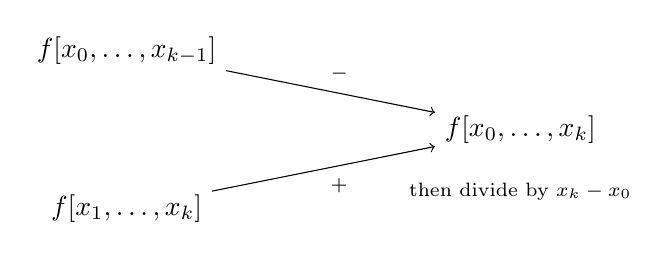
\begin{tikzpicture}
  \node (a) at (0,1.0) {$f[x_0, \dots, x_{k-1}]$};
  \node (b) at (0,-1.0) {$f[x_1, \dots, x_{k}]$};
  \node (c) at (5.0,0) {$f[x_0, \dots, x_{k}]$};
  \draw[->,thin] (a) -- (c);
  \draw[->,thin] (b) -- (c);
  \node[above] at (2.7,0.5) {\scriptsize $-$};
  \node[below] at (2.7,-0.5) {\scriptsize $+$};
  \node[below] at (5.0,-0.55) {\scriptsize then divide by $x_k - x_0$};
\end{tikzpicture}
\end{center}
so that the table is filled column by column, each column being one entry shorter than the last.

Finally evaluation of $p$ at a given point $x$ using Newton formula (provided that divided differences $A_k = f[x_0, \dots, x_k]$ are known) requires just $n$ multiplications, as long as we do it by the \vocab{Horner scheme}
\begin{align*}
p_{n}(x)=&\{\cdots\{\{A_{n} \times(x-x_{n-1})+A_{n-1}\} \times(x-x_{n-2})+A_{n-2}\} \\
& \times(x-x_{n-3})+\cdots+A_{1}\} \times(x-x_{0})+A_{0} .
\end{align*}

It is worth pausing to compare the two forms. Both cost $\mathcal{O}(n^2)$ operations to set up. The Lagrange form is the one to reach for when we want to \emph{manipulate} the interpolant symbolically -- to integrate it, say, or to differentiate it -- because $f$ appears in it linearly, through the values $f(x_i)$, with coefficients $\ell_i$ that do not depend on $f$ at all. This is exactly what we will exploit when we build quadrature rules in Section 3. The Newton form, on the other hand, is the one to reach for when we want to \emph{compute}: adding a new interpolation point $x_{n+1}$ costs only one extra term, whereas in the Lagrange form every single $\ell_i$ has to be recomputed from scratch.

\subsection{Examples}

We will now look at some examples of these methods in use.

\begin{example}[Interpolating Polynomial]
  Given the data
  \begin{center}
    \begin{tabular}{c|r|r|r|r}
      $x_{i}$ & 0 & 1 & 2 & 3 \\
      \hline$f\left(x_{i}\right)$ & $-3$ & $-3$ & $-1$ & 9
      \end{tabular}
  \end{center}
  we want to find the interpolating polynomial $p \in \mathcal{P}_3$ in both Lagrange and Newton forms.

  \emph{Fundamental Lagrange polynomials}. We have
  \begin{align*}
      \ell_{0}(x)&=\frac{(x-1)(x-2)(x-3)}{-6}=-\frac{1}{6}\left(x^{3}-6 x^{2}+11 x-6\right), \\
      \ell_{1}(x)&=\frac{x(x-2)(x-3)}{2}=\frac{1}{2}\left(x^{3}-5 x^{2}+6 x\right), \\
      \ell_{2}(x)&=\frac{x(x-1)(x-3)}{-2}=-\frac{1}{2}\left(x^{3}-4 x^{2}+3 x\right), \\
      \ell_{3}(x)&=\frac{x(x-1)(x-2)}{6}=\frac{1}{6}\left(x^{3}-3 x^{2}+2 x\right) .
  \end{align*}

  \emph{Lagrange form}. Using the polynomials above, we can write
  \begin{align*}
      p(x) &=(-3) \cdot \ell_{0}(x)+(-3) \cdot \ell_{1}(x)+(-1) \cdot \ell_{2}(x)+9 \cdot \ell_{3}(x) \\
      &=\left(\frac{1}{2}-\frac{3}{2}+\frac{1}{2}+\frac{3}{2}\right) x^{3}+\left(-3+\frac{15}{2}-2-\frac{9}{2}\right) x^{2}+\left(\frac{11}{2}-9+\frac{3}{2}+3\right) x-3 \\
      &=x^{3}-2 x^{2}+x-3 .
  \end{align*}

  \emph{Newton form}. Here we build the divided difference table, filling it in column by column using the recurrence \eqref{eq:ddrec}. Since the nodes are spaced one apart, the denominators $x_k - x_0$ are $1, 2, 3$ in the three successive columns.
  \begin{center}
    \begin{tabular}{crrrr}
      \toprule
      $x_i$ & $f[x_i]$ & $f[*,*]$ & $f[*,*,*]$ & $f[*,*,*,*]$\\
      \midrule
      $0$ & $-3$ \\
          &      & $0$ \\
      $1$ & $-3$ &     & $1$\\
          &      & $2$ &     & $1$\\
      $2$ & $-1$ &     & $4$\\
          &      & $10$\\
      $3$ & $9$\\
      \bottomrule
    \end{tabular}
  \end{center}
  Reading off the numbers at the head of each column gives
  $$
  p(x) = -3 + 0 \cdot (x - 0) + 1 \cdot (x-0)(x-1) + 1\cdot (x-0)(x-1)(x-2),
  $$
  and expanding this out we do indeed recover $p(x) = x^3 - 2x^2 + x - 3$, as we must.
\end{example}

Notice how much less work the second computation was. The advantage becomes more pronounced still if the data arrives one point at a time.

\begin{example}[Adding a Point]
  Suppose that to the data of the previous example we now append the point $x_4 = 4$, $f(x_4) = 33$. In the Lagrange form we would have to start again. In the Newton form we merely extend the table by one diagonal:
  $$
  f[x_3, x_4] = \frac{33 - 9}{1} = 24, \quad f[x_2, x_3, x_4] = \frac{24 - 10}{2} = 7, \quad f[x_1, \dots, x_4] = \frac{7 - 4}{2} = \frac{3}{2},
  $$
  and finally $f[x_0, \dots, x_4] = (\tfrac{3}{2} - 1)/4 = \tfrac{1}{8}$. Hence
  $$
  p_4(x) = p_3(x) + \tfrac{1}{8}x(x-1)(x-2)(x-3).
  $$
  All the work done for $p_3$ has been retained.
\end{example}

\begin{example}[A Divided Difference Table with Non-uniform Nodes]
  Let $f(x) = \sqrt{x}$ and take the nodes $x_0 = 1$, $x_1 = 4$, $x_2 = 9$. Then
  $$
  f[x_0, x_1] = \frac{2 - 1}{4 - 1} = \frac{1}{3}, \qquad f[x_1, x_2] = \frac{3 - 2}{9 - 4} = \frac{1}{5},
  $$
  and so
  $$
  f[x_0, x_1, x_2] = \frac{\frac{1}{5} - \frac{1}{3}}{9 - 1} = -\frac{1}{60}.
  $$
  The interpolant is therefore
  $$
  p_2(x) = 1 + \tfrac{1}{3}(x-1) - \tfrac{1}{60}(x-1)(x-4).
  $$
  Evaluating at $x = 2$ gives $p_2(2) = 1 + \tfrac{1}{3} + \tfrac{1}{30} = 1.3\overline{6}$, against the true value $\sqrt{2} = 1.41421\ldots$. The error is about $0.048$, which -- as we are about to see -- is entirely predictable.
\end{example}

\subsection{The Error of Interpolation}

An interpolant is only useful if we can say how far it is from $f$ \emph{between} the interpolation points. The following theorem, which is the workhorse of the whole subject, says that the error looks exactly like the next term of a Taylor series, with the monomial $(x - a)^{n+1}$ replaced by the nodal polynomial $\omega$.

\begin{theorem}[Interpolation Error]\label{thm:interperror}
  Let $f \in C^{n+1}[a, b]$ and let $x_0, \dots, x_n \in [a, b]$ be distinct. Let $p \in \Pn{n}$ interpolate $f$ at these points. Then for every $x \in [a,b]$ there exists $\xi = \xi(x) \in (a,b)$ such that
  $$
  f(x) - p(x) = \frac{1}{(n+1)!}f^{(n+1)}(\xi) \, \omega(x), \qquad \omega(x) = \prod_{i=0}^{n}(x - x_i).
  $$
\end{theorem}
\begin{proof}
  If $x = x_i$ for some $i$ then both sides vanish and there is nothing to prove, so fix $x \in [a,b]$ with $x \neq x_i$ for all $i$. In particular $\omega(x) \neq 0$, so we may define $\varphi : [a,b] \to \R$ by
  $$
  \varphi(t) = f(t) - p(t) - \big(f(x) - p(x)\big)\frac{\omega(t)}{\omega(x)}.
  $$
  This is a $C^{n+1}$ function of $t$, and it has been rigged so that $\varphi(x) = 0$; it also vanishes at each of $x_0, \dots, x_n$, since there $f - p$ and $\omega$ both vanish. So $\varphi$ has at least $n+2$ distinct zeros in $[a,b]$.

  Now we apply Rolle's theorem repeatedly. Between consecutive zeros of $\varphi$ there is a zero of $\varphi'$, so $\varphi'$ has at least $n+1$ distinct zeros; between consecutive zeros of $\varphi'$ there is a zero of $\varphi''$, so $\varphi''$ has at least $n$ distinct zeros; and continuing in this way, $\varphi^{(n+1)}$ has at least one zero, say $\xi \in (a,b)$.

  But $p \in \Pn{n}$ has $p^{(n+1)} \equiv 0$, while $\omega$ is monic of degree $n+1$ and so $\omega^{(n+1)} \equiv (n+1)!$. Hence
  $$
  0 = \varphi^{(n+1)}(\xi) = f^{(n+1)}(\xi) - \big(f(x) - p(x)\big)\frac{(n+1)!}{\omega(x)},
  $$
  and rearranging gives the result.
\end{proof}

The same trick -- count zeros, then apply Rolle -- gives a very satisfying interpretation of divided differences: they are, up to a factorial, derivatives.

\begin{theorem}[Divided Differences and Derivatives]\label{thm:ddderiv}
  Let $x_0, \dots, x_n$ be distinct points and let $[a,b]$ be the smallest interval containing them. If $f \in C^n[a,b]$, then there is some $\xi \in (a, b)$ with
  $$
  f[x_0, \dots, x_n] = \frac{1}{n!}f^{(n)}(\xi).
  $$
\end{theorem}
\begin{proof}
  Let $p \in \Pn{n}$ interpolate $f$ at the $n+1$ points. Then $f - p$ vanishes at $n+1$ distinct points, so by Rolle applied $n$ times, $(f - p)^{(n)}$ vanishes somewhere in $(a,b)$, say at $\xi$. But $p$ has leading coefficient $f[x_0, \dots, x_n]$, so $p^{(n)} \equiv n!\, f[x_0, \dots, x_n]$, and thus
  $$
  0 = f^{(n)}(\xi) - n!\, f[x_0, \dots, x_n]. \qedhere
  $$
\end{proof}

\begin{remark}
  This is a pleasing statement in its own right: it says that the divided difference is a `discrete derivative', and it also lets us make sense of $f[x_0, \dots, x_n]$ when some of the points coalesce. Letting all the $x_i \to x$, the natural definition is $f[x, x, \dots, x] = f^{(n)}(x)/n!$, and with this convention the Newton formula becomes the Taylor expansion of $f$ about $x$. Interpolation and Taylor expansion are, in this sense, the same thing.
\end{remark}

Let us use Theorem \ref{thm:interperror} on the example above.

\begin{example}
  With $f(x) = \sqrt{x}$ and nodes $1, 4, 9$, we have $f'''(x) = \tfrac{3}{8}x^{-5/2}$ and $\omega(2) = (2-1)(2-4)(2-9) = 14$. So
  $$
  \sqrt{2} - p_2(2) = \frac{1}{6}\cdot \frac{3}{8}\xi^{-5/2}\cdot 14 = \frac{7}{8}\xi^{-5/2}
  $$
  for some $\xi \in (1,9)$. Since $\xi > 1$ we get $\abs{\sqrt 2 - p_2(2)} \le 7/8$, which is true but useless; a better bound comes from noticing that $\xi$ is in practice near the interval where the action is. The exact error was $0.0476$, corresponding to $\xi \approx 2.2$. The moral is that the theorem gives the \emph{form} of the error very precisely, but a crude bound on $f^{(n+1)}$ can throw most of that precision away.
\end{example}

\subsection{The Runge Phenomenon}

Theorem \ref{thm:interperror} contains two factors that we might hope to control. The factor $f^{(n+1)}(\xi)/(n+1)!$ is out of our hands -- it is a property of $f$. But the nodal polynomial $\omega$ depends only on where we choose to put our interpolation points, and this we \emph{can} control. The following famous example of Runge shows that the choice matters enormously, and that the obvious choice is a bad one.

\begin{example}[Runge's Example]
  Let $f(x) = (1 + x^2)^{-1}$ on $[-5,5]$, and interpolate at the $n+1$ equally spaced points $x_j = -5 + 10j/n$. Below is the case $n = 10$: the function $f$ is in blue, the interpolant $p_{10}$ in red, with the interpolation points marked.
\begin{center}
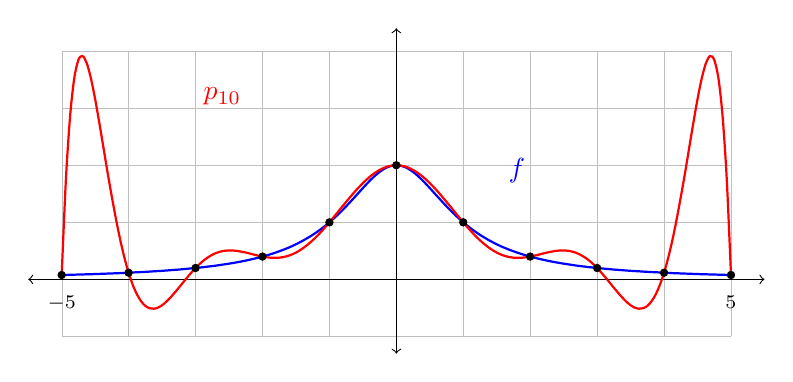
\begin{tikzpicture}
  \draw[ultra thin,color=lightgray] (-4.250,-0.725) -- (-4.250,2.900);
  \draw[ultra thin,color=lightgray] (-3.400,-0.725) -- (-3.400,2.900);
  \draw[ultra thin,color=lightgray] (-2.550,-0.725) -- (-2.550,2.900);
  \draw[ultra thin,color=lightgray] (-1.700,-0.725) -- (-1.700,2.900);
  \draw[ultra thin,color=lightgray] (-0.850,-0.725) -- (-0.850,2.900);
  \draw[ultra thin,color=lightgray] (0.000,-0.725) -- (0.000,2.900);
  \draw[ultra thin,color=lightgray] (0.850,-0.725) -- (0.850,2.900);
  \draw[ultra thin,color=lightgray] (1.700,-0.725) -- (1.700,2.900);
  \draw[ultra thin,color=lightgray] (2.550,-0.725) -- (2.550,2.900);
  \draw[ultra thin,color=lightgray] (3.400,-0.725) -- (3.400,2.900);
  \draw[ultra thin,color=lightgray] (4.250,-0.725) -- (4.250,2.900);
  \draw[ultra thin,color=lightgray] (-4.250,-0.725) -- (4.250,-0.725);
  \draw[ultra thin,color=lightgray] (-4.250,0.000) -- (4.250,0.000);
  \draw[ultra thin,color=lightgray] (-4.250,0.725) -- (4.250,0.725);
  \draw[ultra thin,color=lightgray] (-4.250,1.450) -- (4.250,1.450);
  \draw[ultra thin,color=lightgray] (-4.250,2.175) -- (4.250,2.175);
  \draw[ultra thin,color=lightgray] (-4.250,2.900) -- (4.250,2.900);
  \draw[<->] (-4.675,0) -- (4.675,0);
  \draw[<->] (0,-0.943) -- (0,3.190);
  \draw[thick,smooth,color=blue] plot coordinates {
    (-4.250,0.056) (-4.197,0.057) (-4.144,0.059) (-4.091,0.060) (-4.037,0.062) (-3.984,0.063)
    (-3.931,0.065) (-3.878,0.066) (-3.825,0.068) (-3.772,0.070) (-3.719,0.072) (-3.666,0.074)
    (-3.612,0.076) (-3.559,0.078) (-3.506,0.080) (-3.453,0.083) (-3.400,0.085) (-3.347,0.088)
    (-3.294,0.091) (-3.241,0.093) (-3.188,0.096) (-3.134,0.099) (-3.081,0.103) (-3.028,0.106)
    (-2.975,0.109) (-2.922,0.113) (-2.869,0.117) (-2.816,0.121) (-2.762,0.125) (-2.709,0.130)
    (-2.656,0.135) (-2.603,0.140) (-2.550,0.145) (-2.497,0.151) (-2.444,0.156) (-2.391,0.163)
    (-2.337,0.169) (-2.284,0.176) (-2.231,0.184) (-2.178,0.192) (-2.125,0.200) (-2.072,0.209)
    (-2.019,0.218) (-1.966,0.228) (-1.912,0.239) (-1.859,0.251) (-1.806,0.263) (-1.753,0.276)
    (-1.700,0.290) (-1.647,0.305) (-1.594,0.321) (-1.541,0.338) (-1.488,0.357) (-1.434,0.377)
    (-1.381,0.398) (-1.328,0.421) (-1.275,0.446) (-1.222,0.473) (-1.169,0.502) (-1.116,0.533)
    (-1.062,0.566) (-1.009,0.602) (-0.956,0.640) (-0.903,0.681) (-0.850,0.725) (-0.797,0.772)
    (-0.744,0.821) (-0.691,0.873) (-0.637,0.928) (-0.584,0.985) (-0.531,1.043) (-0.478,1.101)
    (-0.425,1.160) (-0.372,1.217) (-0.319,1.271) (-0.266,1.321) (-0.212,1.365) (-0.159,1.401)
    (-0.106,1.428) (-0.053,1.444) (0.000,1.450) (0.053,1.444) (0.106,1.428) (0.159,1.401)
    (0.212,1.365) (0.266,1.321) (0.319,1.271) (0.372,1.217) (0.425,1.160) (0.478,1.101)
    (0.531,1.043) (0.584,0.985) (0.637,0.928) (0.691,0.873) (0.744,0.821) (0.797,0.772)
    (0.850,0.725) (0.903,0.681) (0.956,0.640) (1.009,0.602) (1.062,0.566) (1.116,0.533)
    (1.169,0.502) (1.222,0.473) (1.275,0.446) (1.328,0.421) (1.381,0.398) (1.434,0.377)
    (1.488,0.357) (1.541,0.338) (1.594,0.321) (1.647,0.305) (1.700,0.290) (1.753,0.276)
    (1.806,0.263) (1.859,0.251) (1.912,0.239) (1.966,0.228) (2.019,0.218) (2.072,0.209)
    (2.125,0.200) (2.178,0.192) (2.231,0.184) (2.284,0.176) (2.337,0.169) (2.391,0.163)
    (2.444,0.156) (2.497,0.151) (2.550,0.145) (2.603,0.140) (2.656,0.135) (2.709,0.130)
    (2.762,0.125) (2.816,0.121) (2.869,0.117) (2.922,0.113) (2.975,0.109) (3.028,0.106)
    (3.081,0.103) (3.134,0.099) (3.188,0.096) (3.241,0.093) (3.294,0.091) (3.347,0.088)
    (3.400,0.085) (3.453,0.083) (3.506,0.080) (3.559,0.078) (3.612,0.076) (3.666,0.074)
    (3.719,0.072) (3.772,0.070) (3.825,0.068) (3.878,0.066) (3.931,0.065) (3.984,0.063)
    (4.037,0.062) (4.091,0.060) (4.144,0.059) (4.197,0.057) (4.250,0.056)
  };
  \draw[thick,smooth,color=red] plot coordinates {
    (-4.250,0.056) (-4.197,1.259) (-4.144,2.064) (-4.091,2.551) (-4.037,2.789) (-3.984,2.837)
    (-3.931,2.744) (-3.878,2.550) (-3.825,2.289) (-3.772,1.988) (-3.719,1.670) (-3.666,1.350)
    (-3.612,1.043) (-3.559,0.758) (-3.506,0.500) (-3.453,0.275) (-3.400,0.085) (-3.347,-0.070)
    (-3.294,-0.190) (-3.241,-0.278) (-3.188,-0.336) (-3.134,-0.366) (-3.081,-0.372)
    (-3.028,-0.359) (-2.975,-0.328) (-2.922,-0.284) (-2.869,-0.230) (-2.816,-0.170)
    (-2.762,-0.105) (-2.709,-0.040) (-2.656,0.025) (-2.603,0.087) (-2.550,0.145) (-2.497,0.197)
    (-2.444,0.243) (-2.391,0.281) (-2.337,0.313) (-2.284,0.337) (-2.231,0.354) (-2.178,0.364)
    (-2.125,0.368) (-2.072,0.367) (-2.019,0.361) (-1.966,0.352) (-1.912,0.341) (-1.859,0.328)
    (-1.806,0.314) (-1.753,0.301) (-1.700,0.290) (-1.647,0.281) (-1.594,0.275) (-1.541,0.274)
    (-1.488,0.276) (-1.434,0.284) (-1.381,0.297) (-1.328,0.316) (-1.275,0.341) (-1.222,0.372)
    (-1.169,0.408) (-1.116,0.450) (-1.062,0.497) (-1.009,0.548) (-0.956,0.604) (-0.903,0.663)
    (-0.850,0.725) (-0.797,0.789) (-0.744,0.854) (-0.691,0.920) (-0.637,0.985) (-0.584,1.048)
    (-0.531,1.110) (-0.478,1.168) (-0.425,1.223) (-0.372,1.273) (-0.319,1.318) (-0.266,1.357)
    (-0.212,1.390) (-0.159,1.416) (-0.106,1.435) (-0.053,1.446) (0.000,1.450) (0.053,1.446)
    (0.106,1.435) (0.159,1.416) (0.212,1.390) (0.266,1.357) (0.319,1.318) (0.372,1.273)
    (0.425,1.223) (0.478,1.168) (0.531,1.110) (0.584,1.048) (0.637,0.985) (0.691,0.920)
    (0.744,0.854) (0.797,0.789) (0.850,0.725) (0.903,0.663) (0.956,0.604) (1.009,0.548)
    (1.062,0.497) (1.116,0.450) (1.169,0.408) (1.222,0.372) (1.275,0.341) (1.328,0.316)
    (1.381,0.297) (1.434,0.284) (1.488,0.276) (1.541,0.274) (1.594,0.275) (1.647,0.281)
    (1.700,0.290) (1.753,0.301) (1.806,0.314) (1.859,0.328) (1.912,0.341) (1.966,0.352)
    (2.019,0.361) (2.072,0.367) (2.125,0.368) (2.178,0.364) (2.231,0.354) (2.284,0.337)
    (2.337,0.313) (2.391,0.281) (2.444,0.243) (2.497,0.197) (2.550,0.145) (2.603,0.087)
    (2.656,0.025) (2.709,-0.040) (2.762,-0.105) (2.816,-0.170) (2.869,-0.230) (2.922,-0.284)
    (2.975,-0.328) (3.028,-0.359) (3.081,-0.372) (3.134,-0.366) (3.188,-0.336) (3.241,-0.278)
    (3.294,-0.190) (3.347,-0.070) (3.400,0.085) (3.453,0.275) (3.506,0.500) (3.559,0.758)
    (3.612,1.043) (3.666,1.350) (3.719,1.670) (3.772,1.988) (3.825,2.289) (3.878,2.550)
    (3.931,2.744) (3.984,2.837) (4.037,2.789) (4.091,2.551) (4.144,2.064) (4.197,1.259)
    (4.250,0.056)
  };
  \filldraw[black] (-4.250,0.056) circle (1.3pt);
  \filldraw[black] (-3.400,0.085) circle (1.3pt);
  \filldraw[black] (-2.550,0.145) circle (1.3pt);
  \filldraw[black] (-1.700,0.290) circle (1.3pt);
  \filldraw[black] (-0.850,0.725) circle (1.3pt);
  \filldraw[black] (0.000,1.450) circle (1.3pt);
  \filldraw[black] (0.850,0.725) circle (1.3pt);
  \filldraw[black] (1.700,0.290) circle (1.3pt);
  \filldraw[black] (2.550,0.145) circle (1.3pt);
  \filldraw[black] (3.400,0.085) circle (1.3pt);
  \filldraw[black] (4.250,0.056) circle (1.3pt);
  \node[color=blue] at (1.530,1.377) {$f$};
  \node[color=red] at (-2.210,2.320) {$p_{10}$};
  \node[below] at (4.250,-0.087) {\scriptsize $5$};
  \node[below] at (-4.250,-0.087) {\scriptsize $-5$};
\end{tikzpicture}
\end{center}

  The interpolant is faithful in the middle of the interval and catastrophically bad near the endpoints, where it oscillates with amplitude close to $2$ even though $\abs{f} \le 1$ everywhere. Worse, this does not improve as $n$ grows: one can show that
  $$
  \max_{x \in [-5,5]}\abs{f(x) - p_n(x)} \to \infty \quad \text{as } n \to \infty.
  $$
  Interpolating at more equally spaced points makes matters \emph{worse}, not better.
\end{example}

What has gone wrong? The culprit is the nodal polynomial. For equally spaced nodes on $[-1,1]$, $\abs{\omega}$ is tiny in the middle of the interval but grows by a factor exponential in $n$ as we approach the ends, so the error bound is wildly non-uniform. If we want $\abs{\omega}$ to be uniformly small, we should not space the nodes uniformly; we should cluster them near the endpoints.

The optimal choice is classical. On $[-1,1]$ the \vocab{Chebyshev points}
$$
x_j = \cos\left(\frac{(n - j)\pi}{n}\right), \qquad j = 0, 1, \dots, n,
$$
are obtained by taking $n+1$ equally spaced points on the upper half of the unit circle and projecting them down onto the real axis. The picture makes the clustering obvious.
\begin{center}
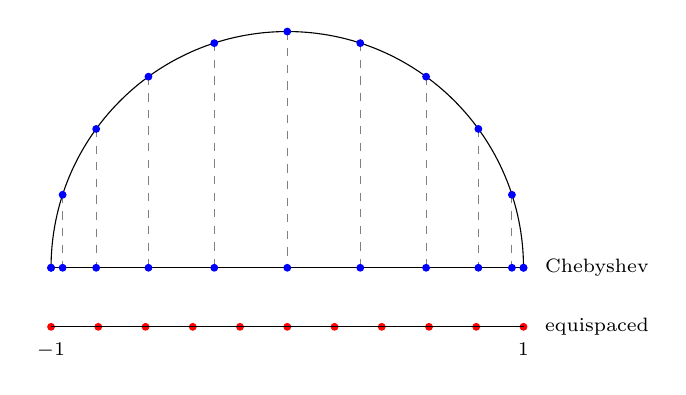
\begin{tikzpicture}
  \draw[thin] (-3.00,0) -- (3.00,0);
  \draw[thin,color=black] (3.00,0) arc (0:180:3.00);
  \draw[thin,dashed,color=gray] (3.000,0.000) -- (3.000,0);
  \draw[thin,dashed,color=gray] (2.853,0.927) -- (2.853,0);
  \draw[thin,dashed,color=gray] (2.427,1.763) -- (2.427,0);
  \draw[thin,dashed,color=gray] (1.763,2.427) -- (1.763,0);
  \draw[thin,dashed,color=gray] (0.927,2.853) -- (0.927,0);
  \draw[thin,dashed,color=gray] (0.000,3.000) -- (0.000,0);
  \draw[thin,dashed,color=gray] (-0.927,2.853) -- (-0.927,0);
  \draw[thin,dashed,color=gray] (-1.763,2.427) -- (-1.763,0);
  \draw[thin,dashed,color=gray] (-2.427,1.763) -- (-2.427,0);
  \draw[thin,dashed,color=gray] (-2.853,0.927) -- (-2.853,0);
  \draw[thin,dashed,color=gray] (-3.000,0.000) -- (-3.000,0);
  \filldraw[color=blue] (3.000,0.000) circle (1.2pt);
  \filldraw[color=blue] (2.853,0.927) circle (1.2pt);
  \filldraw[color=blue] (2.427,1.763) circle (1.2pt);
  \filldraw[color=blue] (1.763,2.427) circle (1.2pt);
  \filldraw[color=blue] (0.927,2.853) circle (1.2pt);
  \filldraw[color=blue] (0.000,3.000) circle (1.2pt);
  \filldraw[color=blue] (-0.927,2.853) circle (1.2pt);
  \filldraw[color=blue] (-1.763,2.427) circle (1.2pt);
  \filldraw[color=blue] (-2.427,1.763) circle (1.2pt);
  \filldraw[color=blue] (-2.853,0.927) circle (1.2pt);
  \filldraw[color=blue] (-3.000,0.000) circle (1.2pt);
  \filldraw[color=blue] (3.000,0) circle (1.2pt);
  \filldraw[color=blue] (2.853,0) circle (1.2pt);
  \filldraw[color=blue] (2.427,0) circle (1.2pt);
  \filldraw[color=blue] (1.763,0) circle (1.2pt);
  \filldraw[color=blue] (0.927,0) circle (1.2pt);
  \filldraw[color=blue] (0.000,0) circle (1.2pt);
  \filldraw[color=blue] (-0.927,0) circle (1.2pt);
  \filldraw[color=blue] (-1.763,0) circle (1.2pt);
  \filldraw[color=blue] (-2.427,0) circle (1.2pt);
  \filldraw[color=blue] (-2.853,0) circle (1.2pt);
  \filldraw[color=blue] (-3.000,0) circle (1.2pt);
  \filldraw[color=red] (-3.000,-0.75) circle (1.2pt);
  \filldraw[color=red] (-2.400,-0.75) circle (1.2pt);
  \filldraw[color=red] (-1.800,-0.75) circle (1.2pt);
  \filldraw[color=red] (-1.200,-0.75) circle (1.2pt);
  \filldraw[color=red] (-0.600,-0.75) circle (1.2pt);
  \filldraw[color=red] (0.000,-0.75) circle (1.2pt);
  \filldraw[color=red] (0.600,-0.75) circle (1.2pt);
  \filldraw[color=red] (1.200,-0.75) circle (1.2pt);
  \filldraw[color=red] (1.800,-0.75) circle (1.2pt);
  \filldraw[color=red] (2.400,-0.75) circle (1.2pt);
  \filldraw[color=red] (3.000,-0.75) circle (1.2pt);
  \draw[thin] (-3.00,-0.75) -- (3.00,-0.75);
  \node[right] at (3.15,0) {\scriptsize Chebyshev};
  \node[right] at (3.15,-0.75) {\scriptsize equispaced};
  \node[below] at (-3.00,-0.83) {\scriptsize $-1$};
  \node[below] at (3.00,-0.83) {\scriptsize $1$};
\end{tikzpicture}
\end{center}

With this choice one can show that the nodal polynomial satisfies
$$
\max_{x \in [-1,1]}\abs{\omega(x)} = 2^{-n},
$$
and that no other choice of $n+1$ nodes does better. (The nodal polynomial for the Chebyshev points is $2^{-n}T_{n+1}$, where $T_{n+1}$ is the Chebyshev polynomial we shall meet in the next section; the optimality is a consequence of its equioscillation.) For a general interval $[a,b]$ we simply rescale, taking
$$
x_j = \frac{a+b}{2} + \frac{b-a}{2}\cos\left(\frac{(n-j)\pi}{n}\right).
$$
Repeating Runge's experiment with Chebyshev points, the interpolant converges uniformly to $f$, and rapidly at that.

\begin{remark}
  This is a good point to pause and notice what the theory has bought us. Nothing about the function $f$ has changed; all we have done is move the sampling points. But the same theorem that predicted disaster for equispaced nodes predicts success for Chebyshev nodes, because it isolates precisely the quantity ($\omega$) that we are free to choose. This pattern -- write down an exact error formula, look at which factor is under our control, and optimise it -- recurs throughout the course, and is the whole idea behind Gaussian quadrature.
\end{remark}


\section{Orthogonal Polynomials}

We now change tack somewhat. Rather than asking for a polynomial that agrees with $f$ at finitely many points, we ask for a polynomial that is close to $f$ \emph{on average}, in the sense of least squares. This turns out to require a good basis for $\Pn{n}$, and the right notion of `good' is orthogonality with respect to a suitable inner product. Orthogonal polynomials are the central objects here, and they will reappear -- somewhat unexpectedly -- as the key to the most accurate quadrature rules there are.

\subsection{Inner Products on Function Spaces}

\begin{definition}[Inner Product]
  Let $V$ be a real vector space. An \vocab{inner product} (or scalar product) on $V$ is a map $\ip{\cdot}{\cdot}: V \times V \to \R$ which is
  \begin{enumerate}[label=(\roman*)]
    \item \emph{symmetric}: $\ip{f}{g} = \ip{g}{f}$ for all $f, g \in V$;
    \item \emph{bilinear}: linear in each argument;
    \item \emph{positive definite}: $\ip{f}{f} \geq 0$ for all $f$, with equality if and only if $f = 0$.
  \end{enumerate}
  We say $f$ and $g$ are \vocab{orthogonal} if $\ip{f}{g} = 0$, and we write $\norm{f} = \ip{f}{f}^{1/2}$ for the induced norm.
\end{definition}

For us $V$ will almost always be a space of functions on an interval, and the inner product will be of the following shape.

\begin{definition}[Weight Function]
  Let $[a,b] \subseteq \R$ (possibly infinite) and let $w : (a,b) \to \R$ be continuous, non-negative, and non-zero except at isolated points, with $\int_a^b w(x)\dd x < \infty$. We call $w$ a \vocab{weight function}, and define
  $$
  \ip{f}{g} = \int_a^b w(x)f(x)g(x)\dd x.
  $$
\end{definition}

The conditions on $w$ are exactly what is needed for this to be an inner product on $C[a,b]$: symmetry and bilinearity are immediate, and if $\ip{f}{f} = \int_a^b w f^2 = 0$ with $wf^2 \geq 0$ continuous, then $wf^2 \equiv 0$, and since $w$ vanishes only at isolated points, $f \equiv 0$ by continuity.

A second, more down-to-earth example is available when we only know $f$ at finitely many points.

\begin{example}[Discrete Inner Product]
  Let $\xi_1, \dots, \xi_m$ be distinct points and set
  $$
  \ip{f}{g} = \sum_{j=1}^{m} f(\xi_j) g(\xi_j).
  $$
  This is symmetric and bilinear, and $\ip{f}{f} = \sum_j f(\xi_j)^2 \geq 0$. It is \emph{not} positive definite on all of $C[a,b]$ -- a function vanishing at every $\xi_j$ has zero norm -- but it \emph{is} positive definite on $\Pn{n}$ provided $n < m$, since a nonzero polynomial of degree at most $n$ cannot vanish at $m > n$ points. This is the inner product relevant to fitting a curve to experimental data.
\end{example}

\subsection{Orthogonal Polynomials}

\begin{definition}[Orthogonal Polynomials]
  A sequence $p_0, p_1, p_2, \dots$ of polynomials is a sequence of \vocab{orthogonal polynomials} with respect to $\ip{\cdot}{\cdot}$ if $\deg p_n = n$ for every $n$, and $\ip{p_n}{p_m} = 0$ whenever $n \neq m$.
\end{definition}

Since $\deg p_n = n$ exactly, the polynomials $p_0, \dots, p_n$ are automatically linearly independent (they have distinct degrees), and so they form an orthogonal \emph{basis} of $\Pn{n}$. This is really the point of the definition: we are constructing a basis of $\Pn{n}$ in which computations decouple.

Of course, orthogonal polynomials are only determined up to scaling, so to speak of \emph{the} orthogonal polynomials we should normalise. The usual convention in this course is to take them \vocab{monic}, that is, with leading coefficient $1$.

\begin{theorem}[Existence and Uniqueness]\label{thm:opexist}
  For any inner product on the space of polynomials there exists a unique sequence of monic orthogonal polynomials $p_0, p_1, \dots$, and these may be constructed by the Gram--Schmidt formula
  $$
  p_{n+1}(x) = x^{n+1} - \sum_{k=0}^{n}\frac{\ip{x^{n+1}}{p_k}}{\ip{p_k}{p_k}}p_k(x).
  $$
\end{theorem}
\begin{proof}
  We induct on $n$. For $n = 0$ the only monic polynomial of degree $0$ is $p_0 \equiv 1$, so existence and uniqueness are clear. Suppose then that $p_0, \dots, p_n$ have been found. Define $p_{n+1}$ by the displayed formula. The subtracted sum lies in $\Pn{n}$, so $p_{n+1}$ is monic of degree $n+1$. For each $j \leq n$, using orthogonality of the $p_k$,
  $$
  \ip{p_{n+1}}{p_j} = \ip{x^{n+1}}{p_j} - \frac{\ip{x^{n+1}}{p_j}}{\ip{p_j}{p_j}}\ip{p_j}{p_j} = 0,
  $$
  so $p_{n+1}$ is orthogonal to $p_0, \dots, p_n$ and hence to all of $\Pn{n}$.

  For uniqueness, suppose $\tilde p_{n+1}$ were another monic polynomial of degree $n+1$ orthogonal to $\Pn{n}$. Then $q = p_{n+1} - \tilde p_{n+1}$ has degree at most $n$, so $q \in \Pn{n}$, and $q$ is orthogonal to everything in $\Pn{n}$ -- in particular to itself. Hence $\ip{q}{q} = 0$ and so $q = 0$.
\end{proof}

\begin{remark}
  Note the characterisation buried in that proof: $p_n$ is the unique monic polynomial of degree $n$ orthogonal to \emph{every} polynomial of lower degree. We will use this form of the statement constantly.
\end{remark}

Gram--Schmidt is a perfectly good proof, but it is a poor algorithm: computing $p_{n+1}$ requires all of $p_0, \dots, p_n$, so the cost grows and rounding errors accumulate. For the inner products we care about there is a far better recurrence, which involves only the previous \emph{two} polynomials.

\subsection{The Three-Term Recurrence}

The key hypothesis is that multiplication by $x$ is self-adjoint. For the weighted-integral inner product this is obvious:
$$
\ip{xf}{g} = \int_a^b w(x)\, x f(x) g(x) \dd x = \ip{f}{xg},
$$
and it holds for the discrete inner product too.

\begin{theorem}[Three-Term Recurrence]\label{thm:threeterm}
  Suppose the inner product satisfies $\ip{xf}{g} = \ip{f}{xg}$ for all polynomials $f, g$. Then the monic orthogonal polynomials satisfy
  $$
  p_{n+1}(x) = (x - \alpha_n)p_n(x) - \beta_n p_{n-1}(x), \qquad n \geq 0,
  $$
  with the conventions $p_{-1} \equiv 0$, $p_0 \equiv 1$, $\beta_0$ arbitrary, and
  $$
  \alpha_n = \frac{\ip{p_n}{xp_n}}{\ip{p_n}{p_n}}, \qquad \beta_n = \frac{\ip{p_n}{p_n}}{\ip{p_{n-1}}{p_{n-1}}} > 0 \quad (n \geq 1).
  $$
\end{theorem}
\begin{proof}
  Both $p_{n+1}$ and $xp_n$ are monic of degree $n+1$, so their difference lies in $\Pn{n}$, and since $p_0, \dots, p_n$ is a basis of $\Pn{n}$ we may write
  $$
  p_{n+1}(x) - xp_n(x) = \sum_{k=0}^{n}\gamma_k p_k(x)
  $$
  for some scalars $\gamma_k$. Taking the inner product with $p_j$ for $j \le n$ and using orthogonality of $p_{n+1}$ against $\Pn{n}$,
  $$
  \gamma_j \ip{p_j}{p_j} = -\ip{xp_n}{p_j} = -\ip{p_n}{xp_j},
  $$
  where the last step is the self-adjointness hypothesis. Now if $j \leq n - 2$ then $xp_j \in \Pn{n-1}$, which is orthogonal to $p_n$, so $\gamma_j = 0$. Only $j = n$ and $j = n-1$ survive, giving
  $$
  p_{n+1}(x) = (x - \alpha_n)p_n(x) - \beta_n p_{n-1}(x), \quad \alpha_n = \frac{\ip{p_n}{xp_n}}{\ip{p_n}{p_n}}, \quad \beta_n = \frac{\ip{p_n}{xp_{n-1}}}{\ip{p_{n-1}}{p_{n-1}}}.
  $$
  Finally, $xp_{n-1}$ is monic of degree $n$, so $xp_{n-1} - p_n \in \Pn{n-1}$ is orthogonal to $p_n$; hence $\ip{p_n}{xp_{n-1}} = \ip{p_n}{p_n}$, which gives the stated $\beta_n$, manifestly positive.
\end{proof}

This is a genuinely useful algorithm: each new polynomial costs $\mathcal{O}(1)$ inner products rather than $\mathcal{O}(n)$, and the recurrence is numerically stable. Let's look at the two examples that matter most.

\begin{example}[Legendre Polynomials]
  Take $[a,b] = [-1,1]$ and $w \equiv 1$, so that $\ip{f}{g} = \int_{-1}^1 fg \dd x$. The resulting monic orthogonal polynomials are the (monic) \vocab{Legendre polynomials}. By symmetry $\ip{p_n}{xp_n} = 0$ for every $n$ -- the integrand is odd -- so $\alpha_n = 0$ throughout, and the recurrence collapses to $p_{n+1} = xp_n - \beta_n p_{n-1}$. Computing,
  $$
  p_0 = 1, \quad p_1 = x, \quad p_2 = x^2 - \tfrac{1}{3}, \quad p_3 = x^3 - \tfrac{3}{5}x, \quad p_4 = x^4 - \tfrac{6}{7}x^2 + \tfrac{3}{35}.
  $$
  For instance $\beta_1 = \ip{p_1}{p_1}/\ip{p_0}{p_0} = (2/3)/2 = 1/3$, giving $p_2 = x \cdot x - \tfrac13 = x^2 - \tfrac13$ as claimed. In the literature one usually meets these normalised so that $P_n(1) = 1$; then $P_0 = 1$, $P_1 = x$, $P_2 = \tfrac12(3x^2 - 1)$, and so on.
\end{example}

\begin{example}[Chebyshev Polynomials]
  Take $[a,b] = [-1,1]$ with the weight $w(x) = (1-x^2)^{-1/2}$, so
  $$
  \ip{f}{g} = \int_{-1}^{1}\frac{f(x)g(x)}{\sqrt{1-x^2}}\dd x.
  $$
  (The weight blows up at $\pm 1$, but integrably, so this is fine.) Define $T_n$ by
  $$
  T_n(\cos\theta) = \cos(n\theta).
  $$
  That this really is a polynomial in $x = \cos\theta$ follows by induction from the identity $\cos((n+1)\theta) + \cos((n-1)\theta) = 2\cos\theta\cos(n\theta)$, which gives at once the recurrence
  $$
  T_{n+1}(x) = 2xT_n(x) - T_{n-1}(x), \qquad T_0 = 1, \; T_1 = x.
  $$
  So $T_2 = 2x^2 - 1$, $T_3 = 4x^3 - 3x$, $T_4 = 8x^4 - 8x^2 + 1$, and in general $T_n$ has leading coefficient $2^{n-1}$ for $n \geq 1$.

  To see orthogonality, substitute $x = \cos\theta$, $\dd x = -\sin\theta \dd\theta$, $\sqrt{1-x^2} = \sin\theta$:
  $$
  \ip{T_n}{T_m} = \int_{-1}^{1}\frac{T_n T_m}{\sqrt{1-x^2}}\dd x = \int_0^\pi \cos(n\theta)\cos(m\theta)\dd\theta = 0
  $$
  for $n \neq m$, by the usual orthogonality of cosines. The monic Chebyshev polynomials are $2^{1-n}T_n$ for $n \ge 1$.
\end{example}

The Chebyshev polynomials are worth a picture, because their defining feature is visible at a glance: on $[-1,1]$ they oscillate between $-1$ and $+1$, attaining those extreme values $n+1$ times.
\begin{center}
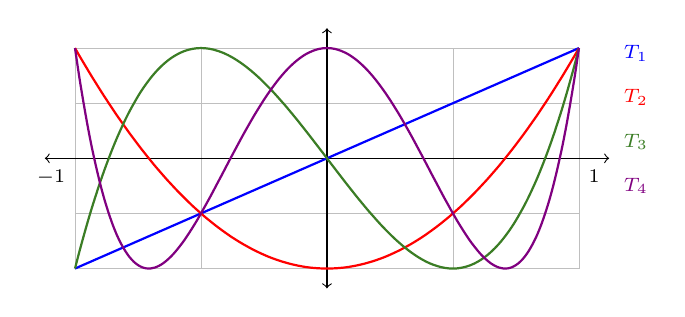
\begin{tikzpicture}
  \draw[ultra thin,color=lightgray] (-3.200,-1.400) -- (-3.200,1.400);
  \draw[ultra thin,color=lightgray] (-1.600,-1.400) -- (-1.600,1.400);
  \draw[ultra thin,color=lightgray] (0.000,-1.400) -- (0.000,1.400);
  \draw[ultra thin,color=lightgray] (1.600,-1.400) -- (1.600,1.400);
  \draw[ultra thin,color=lightgray] (3.200,-1.400) -- (3.200,1.400);
  \draw[ultra thin,color=lightgray] (-3.200,-1.400) -- (3.200,-1.400);
  \draw[ultra thin,color=lightgray] (-3.200,-0.700) -- (3.200,-0.700);
  \draw[ultra thin,color=lightgray] (-3.200,0.000) -- (3.200,0.000);
  \draw[ultra thin,color=lightgray] (-3.200,0.700) -- (3.200,0.700);
  \draw[ultra thin,color=lightgray] (-3.200,1.400) -- (3.200,1.400);
  \draw[<->] (-3.584,0) -- (3.584,0);
  \draw[<->] (0,-1.652) -- (0,1.652);
  \draw[thick,smooth,color=blue] plot coordinates {
    (-3.200,-1.400) (-3.147,-1.377) (-3.093,-1.353) (-3.040,-1.330) (-2.987,-1.307)
    (-2.933,-1.283) (-2.880,-1.260) (-2.827,-1.237) (-2.773,-1.213) (-2.720,-1.190)
    (-2.667,-1.167) (-2.613,-1.143) (-2.560,-1.120) (-2.507,-1.097) (-2.453,-1.073)
    (-2.400,-1.050) (-2.347,-1.027) (-2.293,-1.003) (-2.240,-0.980) (-2.187,-0.957)
    (-2.133,-0.933) (-2.080,-0.910) (-2.027,-0.887) (-1.973,-0.863) (-1.920,-0.840)
    (-1.867,-0.817) (-1.813,-0.793) (-1.760,-0.770) (-1.707,-0.747) (-1.653,-0.723)
    (-1.600,-0.700) (-1.547,-0.677) (-1.493,-0.653) (-1.440,-0.630) (-1.387,-0.607)
    (-1.333,-0.583) (-1.280,-0.560) (-1.227,-0.537) (-1.173,-0.513) (-1.120,-0.490)
    (-1.067,-0.467) (-1.013,-0.443) (-0.960,-0.420) (-0.907,-0.397) (-0.853,-0.373)
    (-0.800,-0.350) (-0.747,-0.327) (-0.693,-0.303) (-0.640,-0.280) (-0.587,-0.257)
    (-0.533,-0.233) (-0.480,-0.210) (-0.427,-0.187) (-0.373,-0.163) (-0.320,-0.140)
    (-0.267,-0.117) (-0.213,-0.093) (-0.160,-0.070) (-0.107,-0.047) (-0.053,-0.023)
    (0.000,0.000) (0.053,0.023) (0.107,0.047) (0.160,0.070) (0.213,0.093) (0.267,0.117)
    (0.320,0.140) (0.373,0.163) (0.427,0.187) (0.480,0.210) (0.533,0.233) (0.587,0.257)
    (0.640,0.280) (0.693,0.303) (0.747,0.327) (0.800,0.350) (0.853,0.373) (0.907,0.397)
    (0.960,0.420) (1.013,0.443) (1.067,0.467) (1.120,0.490) (1.173,0.513) (1.227,0.537)
    (1.280,0.560) (1.333,0.583) (1.387,0.607) (1.440,0.630) (1.493,0.653) (1.547,0.677)
    (1.600,0.700) (1.653,0.723) (1.707,0.747) (1.760,0.770) (1.813,0.793) (1.867,0.817)
    (1.920,0.840) (1.973,0.863) (2.027,0.887) (2.080,0.910) (2.133,0.933) (2.187,0.957)
    (2.240,0.980) (2.293,1.003) (2.347,1.027) (2.400,1.050) (2.453,1.073) (2.507,1.097)
    (2.560,1.120) (2.613,1.143) (2.667,1.167) (2.720,1.190) (2.773,1.213) (2.827,1.237)
    (2.880,1.260) (2.933,1.283) (2.987,1.307) (3.040,1.330) (3.093,1.353) (3.147,1.377)
    (3.200,1.400)
  };
  \draw[thick,smooth,color=red] plot coordinates {
    (-3.200,1.400) (-3.147,1.307) (-3.093,1.216) (-3.040,1.127) (-2.987,1.039) (-2.933,0.953)
    (-2.880,0.868) (-2.827,0.785) (-2.773,0.703) (-2.720,0.623) (-2.667,0.544) (-2.613,0.467)
    (-2.560,0.392) (-2.507,0.318) (-2.453,0.246) (-2.400,0.175) (-2.347,0.106) (-2.293,0.038)
    (-2.240,-0.028) (-2.187,-0.093) (-2.133,-0.156) (-2.080,-0.217) (-2.027,-0.277)
    (-1.973,-0.335) (-1.920,-0.392) (-1.867,-0.447) (-1.813,-0.501) (-1.760,-0.553)
    (-1.707,-0.604) (-1.653,-0.653) (-1.600,-0.700) (-1.547,-0.746) (-1.493,-0.790)
    (-1.440,-0.833) (-1.387,-0.874) (-1.333,-0.914) (-1.280,-0.952) (-1.227,-0.989)
    (-1.173,-1.024) (-1.120,-1.057) (-1.067,-1.089) (-1.013,-1.119) (-0.960,-1.148)
    (-0.907,-1.175) (-0.853,-1.201) (-0.800,-1.225) (-0.747,-1.248) (-0.693,-1.269)
    (-0.640,-1.288) (-0.587,-1.306) (-0.533,-1.322) (-0.480,-1.337) (-0.427,-1.350)
    (-0.373,-1.362) (-0.320,-1.372) (-0.267,-1.381) (-0.213,-1.388) (-0.160,-1.393)
    (-0.107,-1.397) (-0.053,-1.399) (0.000,-1.400) (0.053,-1.399) (0.107,-1.397) (0.160,-1.393)
    (0.213,-1.388) (0.267,-1.381) (0.320,-1.372) (0.373,-1.362) (0.427,-1.350) (0.480,-1.337)
    (0.533,-1.322) (0.587,-1.306) (0.640,-1.288) (0.693,-1.269) (0.747,-1.248) (0.800,-1.225)
    (0.853,-1.201) (0.907,-1.175) (0.960,-1.148) (1.013,-1.119) (1.067,-1.089) (1.120,-1.057)
    (1.173,-1.024) (1.227,-0.989) (1.280,-0.952) (1.333,-0.914) (1.387,-0.874) (1.440,-0.833)
    (1.493,-0.790) (1.547,-0.746) (1.600,-0.700) (1.653,-0.653) (1.707,-0.604) (1.760,-0.553)
    (1.813,-0.501) (1.867,-0.447) (1.920,-0.392) (1.973,-0.335) (2.027,-0.277) (2.080,-0.217)
    (2.133,-0.156) (2.187,-0.093) (2.240,-0.028) (2.293,0.038) (2.347,0.106) (2.400,0.175)
    (2.453,0.246) (2.507,0.318) (2.560,0.392) (2.613,0.467) (2.667,0.544) (2.720,0.623)
    (2.773,0.703) (2.827,0.785) (2.880,0.868) (2.933,0.953) (2.987,1.039) (3.040,1.127)
    (3.093,1.216) (3.147,1.307) (3.200,1.400)
  };
  \draw[thick,smooth,color=OliveGreen] plot coordinates {
    (-3.200,-1.400) (-3.147,-1.195) (-3.093,-0.998) (-3.040,-0.811) (-2.987,-0.633)
    (-2.933,-0.463) (-2.880,-0.302) (-2.827,-0.150) (-2.773,-0.005) (-2.720,0.131)
    (-2.667,0.259) (-2.613,0.380) (-2.560,0.493) (-2.507,0.598) (-2.453,0.696) (-2.400,0.788)
    (-2.347,0.872) (-2.293,0.949) (-2.240,1.019) (-2.187,1.083) (-2.133,1.141) (-2.080,1.192)
    (-2.027,1.237) (-1.973,1.277) (-1.920,1.310) (-1.867,1.338) (-1.813,1.361) (-1.760,1.378)
    (-1.707,1.390) (-1.653,1.398) (-1.600,1.400) (-1.547,1.398) (-1.493,1.391) (-1.440,1.380)
    (-1.387,1.364) (-1.333,1.345) (-1.280,1.322) (-1.227,1.295) (-1.173,1.264) (-1.120,1.230)
    (-1.067,1.193) (-1.013,1.152) (-0.960,1.109) (-0.907,1.063) (-0.853,1.014) (-0.800,0.962)
    (-0.747,0.909) (-0.693,0.853) (-0.640,0.795) (-0.587,0.735) (-0.533,0.674) (-0.480,0.611)
    (-0.427,0.547) (-0.373,0.481) (-0.320,0.414) (-0.267,0.347) (-0.213,0.278) (-0.160,0.209)
    (-0.107,0.140) (-0.053,0.070) (0.000,-0.000) (0.053,-0.070) (0.107,-0.140) (0.160,-0.209)
    (0.213,-0.278) (0.267,-0.347) (0.320,-0.414) (0.373,-0.481) (0.427,-0.547) (0.480,-0.611)
    (0.533,-0.674) (0.587,-0.735) (0.640,-0.795) (0.693,-0.853) (0.747,-0.909) (0.800,-0.962)
    (0.853,-1.014) (0.907,-1.063) (0.960,-1.109) (1.013,-1.152) (1.067,-1.193) (1.120,-1.230)
    (1.173,-1.264) (1.227,-1.295) (1.280,-1.322) (1.333,-1.345) (1.387,-1.364) (1.440,-1.380)
    (1.493,-1.391) (1.547,-1.398) (1.600,-1.400) (1.653,-1.398) (1.707,-1.390) (1.760,-1.378)
    (1.813,-1.361) (1.867,-1.338) (1.920,-1.310) (1.973,-1.277) (2.027,-1.237) (2.080,-1.192)
    (2.133,-1.141) (2.187,-1.083) (2.240,-1.019) (2.293,-0.949) (2.347,-0.872) (2.400,-0.788)
    (2.453,-0.696) (2.507,-0.598) (2.560,-0.493) (2.613,-0.380) (2.667,-0.259) (2.720,-0.131)
    (2.773,0.005) (2.827,0.150) (2.880,0.302) (2.933,0.463) (2.987,0.633) (3.040,0.811)
    (3.093,0.998) (3.147,1.195) (3.200,1.400)
  };
  \draw[thick,smooth,color=Purple] plot coordinates {
    (-3.200,1.400) (-3.147,1.042) (-3.093,0.714) (-3.040,0.414) (-2.987,0.143) (-2.933,-0.103)
    (-2.880,-0.324) (-2.827,-0.520) (-2.773,-0.694) (-2.720,-0.846) (-2.667,-0.977)
    (-2.613,-1.088) (-2.560,-1.180) (-2.507,-1.255) (-2.453,-1.314) (-2.400,-1.356)
    (-2.347,-1.384) (-2.293,-1.398) (-2.240,-1.399) (-2.187,-1.388) (-2.133,-1.365)
    (-2.080,-1.333) (-2.027,-1.290) (-1.973,-1.239) (-1.920,-1.180) (-1.867,-1.114)
    (-1.813,-1.042) (-1.760,-0.963) (-1.707,-0.880) (-1.653,-0.792) (-1.600,-0.700)
    (-1.547,-0.605) (-1.493,-0.508) (-1.440,-0.409) (-1.387,-0.308) (-1.333,-0.207)
    (-1.280,-0.105) (-1.227,-0.004) (-1.173,0.097) (-1.120,0.196) (-1.067,0.294) (-1.013,0.390)
    (-0.960,0.483) (-0.907,0.573) (-0.853,0.660) (-0.800,0.744) (-0.747,0.823) (-0.693,0.899)
    (-0.640,0.970) (-0.587,1.036) (-0.533,1.098) (-0.480,1.154) (-0.427,1.204) (-0.373,1.250)
    (-0.320,1.289) (-0.267,1.323) (-0.213,1.350) (-0.160,1.372) (-0.107,1.388) (-0.053,1.397)
    (0.000,1.400) (0.053,1.397) (0.107,1.388) (0.160,1.372) (0.213,1.350) (0.267,1.323)
    (0.320,1.289) (0.373,1.250) (0.427,1.204) (0.480,1.154) (0.533,1.098) (0.587,1.036)
    (0.640,0.970) (0.693,0.899) (0.747,0.823) (0.800,0.744) (0.853,0.660) (0.907,0.573)
    (0.960,0.483) (1.013,0.390) (1.067,0.294) (1.120,0.196) (1.173,0.097) (1.227,-0.004)
    (1.280,-0.105) (1.333,-0.207) (1.387,-0.308) (1.440,-0.409) (1.493,-0.508) (1.547,-0.605)
    (1.600,-0.700) (1.653,-0.792) (1.707,-0.880) (1.760,-0.963) (1.813,-1.042) (1.867,-1.114)
    (1.920,-1.180) (1.973,-1.239) (2.027,-1.290) (2.080,-1.333) (2.133,-1.365) (2.187,-1.388)
    (2.240,-1.399) (2.293,-1.398) (2.347,-1.384) (2.400,-1.356) (2.453,-1.314) (2.507,-1.255)
    (2.560,-1.180) (2.613,-1.088) (2.667,-0.977) (2.720,-0.846) (2.773,-0.694) (2.827,-0.520)
    (2.880,-0.324) (2.933,-0.103) (2.987,0.143) (3.040,0.414) (3.093,0.714) (3.147,1.042)
    (3.200,1.400)
  };
  \node[below left] at (-3.200,-0.028) {\scriptsize $-1$};
  \node[below right] at (3.200,-0.028) {\scriptsize $1$};
  \node[color=blue,right] at (3.648,1.330) {\scriptsize $T_1$};
  \node[color=red,right] at (3.648,0.770) {\scriptsize $T_2$};
  \node[color=OliveGreen,right] at (3.648,0.210) {\scriptsize $T_3$};
  \node[color=Purple,right] at (3.648,-0.350) {\scriptsize $T_4$};
\end{tikzpicture}
\end{center}

This \emph{equioscillation} is precisely why the Chebyshev points of the previous section are optimal interpolation nodes: among all monic polynomials of degree $n$, the monic Chebyshev polynomial $2^{1-n}T_n$ is the one with the smallest maximum modulus on $[-1,1]$, namely $2^{1-n}$. Any other monic $q$ of degree $n$ with $\norm{q}_\infty < 2^{1-n}$ would have $2^{1-n}T_n - q$ alternating in sign at the $n+1$ extrema of $T_n$, hence having $n$ zeros -- impossible for a polynomial of degree $n - 1$ that is not identically zero.

There are other classical families, each attached to its own weight, which we mention for completeness:
\begin{center}
  \begin{tabular}{lll}
    \toprule
    Family & Interval & Weight $w(x)$ \\
    \midrule
    Legendre & $[-1,1]$ & $1$ \\
    Chebyshev & $[-1,1]$ & $(1-x^2)^{-1/2}$ \\
    Laguerre & $[0,\infty)$ & $e^{-x}$ \\
    Hermite & $(-\infty,\infty)$ & $e^{-x^2}$ \\
    \bottomrule
  \end{tabular}
\end{center}

\subsection{Least-Squares Approximation by Polynomials}

We can now solve the approximation problem we set out with. Given $f$ and an inner product, we seek the $p \in \Pn{n}$ minimising $\norm{f - p}$. Since $\Pn{n}$ is a finite-dimensional subspace, the answer is of course the orthogonal projection of $f$ onto it -- and having an orthogonal basis to hand makes that projection completely explicit.

\begin{theorem}[Least-Squares Approximation]\label{thm:lsq}
  Let $p_0, p_1, \dots$ be the orthogonal polynomials for $\ip{\cdot}{\cdot}$. Then the unique minimiser of $\norm{f - p}$ over $p \in \Pn{n}$ is
  $$
  \hat p_n = \sum_{k=0}^{n}\frac{\ip{f}{p_k}}{\ip{p_k}{p_k}}p_k.
  $$
\end{theorem}
\begin{proof}
  Any $p \in \Pn{n}$ may be written $p = \sum_{k=0}^n c_k p_k$. Expanding and using orthogonality,
  \begin{align*}
    \norm{f - p}^2 &= \ip{f - \textstyle\sum_k c_kp_k}{f - \textstyle\sum_k c_kp_k}\\
    &= \ip{f}{f} - 2\sum_{k=0}^n c_k \ip{f}{p_k} + \sum_{k=0}^n c_k^2 \ip{p_k}{p_k}.
  \end{align*}
  The cross terms $\ip{p_j}{p_k}$ with $j \neq k$ have vanished, so this is a sum of $n+1$ independent quadratics in the $c_k$. Completing the square in each,
  $$
  \norm{f-p}^2 = \ip{f}{f} - \sum_{k=0}^n \frac{\ip{f}{p_k}^2}{\ip{p_k}{p_k}} + \sum_{k=0}^n \ip{p_k}{p_k}\left(c_k - \frac{\ip{f}{p_k}}{\ip{p_k}{p_k}}\right)^2 .
  $$
  Since $\ip{p_k}{p_k} > 0$, this is minimised precisely when every bracket vanishes, i.e.\ $c_k = \ip{f}{p_k}/\ip{p_k}{p_k}$, and the minimiser is unique.
\end{proof}

Notice the structural virtue of this answer: the coefficient of $p_k$ does not depend on $n$. If we decide we want a better approximation, we simply compute one more coefficient and append one more term; nothing already computed is wasted. This is exactly the adaptivity we admired in the Newton form.

Reading off the value at the minimum in the proof gives the error, and this is worth recording separately.

\begin{corollary}[Bessel's Inequality and Pythagoras]
  With $\hat p_n$ as above,
  $$
  \norm{f - \hat p_n}^2 = \ip{f}{f} - \sum_{k=0}^n \frac{\ip{f}{p_k}^2}{\ip{p_k}{p_k}} = \norm{f}^2 - \norm{\hat p_n}^2 .
  $$
  In particular $\sum_{k=0}^n \ip{f}{p_k}^2/\ip{p_k}{p_k} \leq \norm{f}^2$, and $\ip{f - \hat p_n}{\hat p_n} = 0$.
\end{corollary}

That last statement -- the error is orthogonal to the approximation -- is Pythagoras' theorem, and it is the geometric content of the whole business. It also gives an alternative one-line proof of the theorem: for any $p \in \Pn{n}$ we have $f - p = (f - \hat p_n) + (\hat p_n - p)$ with the two summands orthogonal, so $\norm{f-p}^2 = \norm{f - \hat p_n}^2 + \norm{\hat p_n - p}^2 \geq \norm{f - \hat p_n}^2$.

Since $\norm{f - \hat p_n}$ is decreasing in $n$, it converges; the natural question is whether it converges to zero. It does, and the reason is a theorem from outside numerical analysis entirely.

\begin{theorem}[Weierstrass Approximation Theorem]
  Let $f \in C[a,b]$ with $[a,b]$ finite. For every $\varepsilon > 0$ there is a polynomial $q$ with $\abs{f(x) - q(x)} < \varepsilon$ for all $x \in [a,b]$.
\end{theorem}

We shall not prove this here -- it is a piece of analysis rather than numerical analysis, and the reader will meet it elsewhere. What we want is the consequence.

\begin{corollary}[Convergence of Least-Squares Approximation]
  Let $\ip{f}{g} = \int_a^b w f g \dd x$ with $[a,b]$ finite and $w$ a weight function. Then for $f \in C[a,b]$ we have $\norm{f - \hat p_n} \to 0$ as $n \to \infty$.
\end{corollary}
\begin{proof}
  Let $\varepsilon > 0$ and set $W = \int_a^b w(x)\dd x < \infty$. By Weierstrass there is a polynomial $q$, of degree $m$ say, with $\abs{f - q} < \varepsilon$ pointwise on $[a,b]$. Then
  $$
  \norm{f - q}^2 = \int_a^b w(x)(f(x)-q(x))^2 \dd x \leq \varepsilon^2 W.
  $$
  For $n \geq m$ we have $q \in \Pn{n}$, so by minimality $\norm{f - \hat p_n} \leq \norm{f - q} \leq \varepsilon \sqrt{W}$. As $\varepsilon$ was arbitrary and $\norm{f - \hat p_n}$ is non-increasing, the result follows.
\end{proof}

\begin{corollary}[Parseval's Identity]
  Under the hypotheses above,
  $$
  \sum_{k=0}^\infty \frac{\ip{f}{p_k}^2}{\ip{p_k}{p_k}} = \ip{f}{f}.
  $$
\end{corollary}
\begin{proof}
  Immediate from $\norm{f}^2 - \sum_{k=0}^n \ip{f}{p_k}^2/\ip{p_k}{p_k} = \norm{f - \hat p_n}^2 \to 0$.
\end{proof}

\begin{example}[Least Squares Fit of $\abs{x}$]
  Take $[a,b] = [-1,1]$, $w \equiv 1$, and $f(x) = \abs{x}$, and let us find the best quadratic approximation. Using the monic Legendre polynomials $p_0 = 1$, $p_1 = x$, $p_2 = x^2 - \tfrac13$, we compute
  $$
  \ip{f}{p_0} = \int_{-1}^1 \abs{x} \dd x = 1, \qquad \ip{f}{p_1} = \int_{-1}^1 \abs{x}\, x \dd x = 0,
  $$
  $$
  \ip{f}{p_2} = \int_{-1}^1 \abs{x}\left(x^2 - \tfrac13\right)\dd x = 2\int_0^1\left(x^3 - \tfrac{x}{3}\right)\dd x = 2\left(\tfrac14 - \tfrac16\right) = \tfrac16 .
  $$
  Also $\ip{p_0}{p_0} = 2$ and $\ip{p_2}{p_2} = \int_{-1}^1 (x^2 - \tfrac13)^2\dd x = \tfrac{8}{45}$. Hence
  $$
  \hat p_2(x) = \tfrac12 + \tfrac{1/6}{8/45}\left(x^2 - \tfrac13\right) = \tfrac{15}{16}x^2 + \tfrac{3}{16}.
  $$
  A quick sanity check: $\hat p_2(\pm 1) = 18/16 > 1$ and $\hat p_2(0) = 3/16 > 0$, so the fit overshoots at the ends and at the kink, which is what one expects of a smooth curve chasing a corner.
\end{example}

\subsection{Least Squares with Discrete Data}

In practice one rarely knows $f$ everywhere; one knows $m$ measurements $f(\xi_1), \dots, f(\xi_m)$ at distinct points and wants the $p \in \Pn{n}$ minimising
$$
\sum_{j=1}^m \big(f(\xi_j) - p(\xi_j)\big)^2 .
$$
This is precisely the least-squares problem for the discrete inner product
$$
\ip{g}{h} = \sum_{j=1}^m g(\xi_j)h(\xi_j),
$$
which as we noted is a genuine inner product on $\Pn{n}$ as long as $n < m$. Everything above goes through verbatim: we build the orthogonal polynomials $p_0, \dots, p_n$ for this inner product using the three-term recurrence, which applies because multiplication by $x$ is again self-adjoint, and then Theorem \ref{thm:lsq} hands us the answer.

\begin{remark}
  The naive alternative is to write $p = \sum_k c_k x^k$ and solve the resulting $(n+1) \times (n+1)$ linear system for the $c_k$ -- the so-called \emph{normal equations}. This works, but the matrix involved is close to the notorious Hilbert matrix and is horribly ill-conditioned even for modest $n$. Orthogonalising first turns the linear system into a diagonal one, and the improvement in accuracy is dramatic. We will meet the same phenomenon again, from a different direction, when we discuss the QR factorisation in Section \ref{sec:qr}.
\end{remark}


\section{Approximation of Linear Functionals}

Almost every quantity we might want to extract from a function -- its value at a point, its derivative there, its integral over an interval -- is a \emph{linear} function of $f$. This section is about approximating such quantities using only the simplest data of all, namely point values of $f$.

\begin{definition}[Linear Functional]
  A \vocab{linear functional} on a real vector space $V$ of functions is a linear map $L: V \to \R$.
\end{definition}

We usually do not fuss over the space $V$; we write down a formula for $L$ and take $V$ to be whatever space of functions makes the formula sensible.

\begin{example}
  The following are all linear functionals.
  \begin{enumerate}[label=(\roman*)]
    \item $L(f) = f(\xi)$ for some fixed $\xi$, on $V = C[a,b]$.
    \item $L(f) = f'(\eta)$ for some fixed $\eta$, on $V = C^1[a,b]$.
    \item $L(f) = \int_a^b w(x)f(x)\dd x$, on $V = C[a,b]$.
    \item Any linear combination of the above, for instance
    $$
    L(f) = f(\beta) - f(\alpha) - \frac{\beta - \alpha}{2}\big(f'(\beta) + f'(\alpha)\big).
    $$
  \end{enumerate}
\end{example}

Our aim is to approximate a complicated $L$ (typically an integral) by a finite combination of simple ones,
$$
L(f) \approx \sum_{i=0}^{N} a_i f(x_i),
$$
where $x_0, \dots, x_N \in [a,b]$ are distinct. How should we choose the $a_i$, and the $x_i$?

The natural idea is one we already have: replace $f$ by its interpolating polynomial and apply $L$ to that. Using the fundamental Lagrange polynomials for the nodes $x_i$,
$$
f(x) \approx \sum_{i=0}^N f(x_i)\ell_i(x) \quad \implies \quad L(f) \approx \sum_{i=0}^N L(\ell_i)f(x_i),
$$
so we should take $a_i = L(\ell_i)$. With this choice the approximation is \emph{exact} for $f \in \Pn{N}$, since then the interpolant is $f$ itself.

That is $N+1$ free parameters buying exactness on an $(N+1)$-dimensional space, which sounds like a fair deal. But we have another $N+1$ parameters that we have not used at all -- the nodes $x_i$. If we choose those cleverly too, we might hope for exactness on $\Pn{2N+1}$. Remarkably, for integrals we can achieve exactly that. This is Gaussian quadrature, and it is the subject of the rest of this section.

\subsection{Newton--Cotes Formulae}

First, though, let us see what the naive choice gives. If we take the nodes to be equally spaced and $L(f) = \int_a^b f$, the resulting rules are the classical \vocab{Newton--Cotes formulae}.

\begin{definition}[Newton--Cotes]
  Fix $\nu \ge 1$ and let $x_i = a + i(b-a)/\nu$ for $i = 0, \dots, \nu$. The closed Newton--Cotes rule of order $\nu$ is
  $$
  \int_a^b f(x)\dd x \approx \sum_{i=0}^{\nu} a_i f(x_i), \qquad a_i = \int_a^b \ell_i(x)\dd x .
  $$
\end{definition}

\begin{example}[The Trapezoidal Rule]
  With $\nu = 1$ we have $\ell_0(x) = (b-x)/(b-a)$ and $\ell_1(x) = (x-a)/(b-a)$, each of which integrates to $(b-a)/2$. Hence
  $$
  \int_a^b f(x)\dd x \approx \frac{b-a}{2}\big(f(a) + f(b)\big),
  $$
  which is just the area of the trapezium under the chord joining the two endpoints.
\end{example}

\begin{example}[Simpson's Rule]
  With $\nu = 2$ and nodes $a$, $m = (a+b)/2$, $b$, a short computation gives $a_0 = a_2 = (b-a)/6$ and $a_1 = 2(b-a)/3$, so
  $$
  \int_a^b f(x)\dd x \approx \frac{b-a}{6}\left(f(a) + 4f\left(\frac{a+b}{2}\right) + f(b)\right).
  $$
  By construction this is exact for $f \in \Pn{2}$. In fact it is exact for $f \in \Pn{3}$: taking $[a,b] = [-1,1]$ for convenience, $\int_{-1}^1 x^3 \dd x = 0$ and the rule returns $\tfrac13(-1 + 0 + 1) = 0$ as well. This extra order `for free' is a general feature of Newton--Cotes rules with an even number of subintervals, and comes from the symmetry of the nodes.
\end{example}

Geometrically, the trapezoidal rule replaces $f$ by a chord and Simpson's rule replaces it by a parabola through three points:
\begin{center}
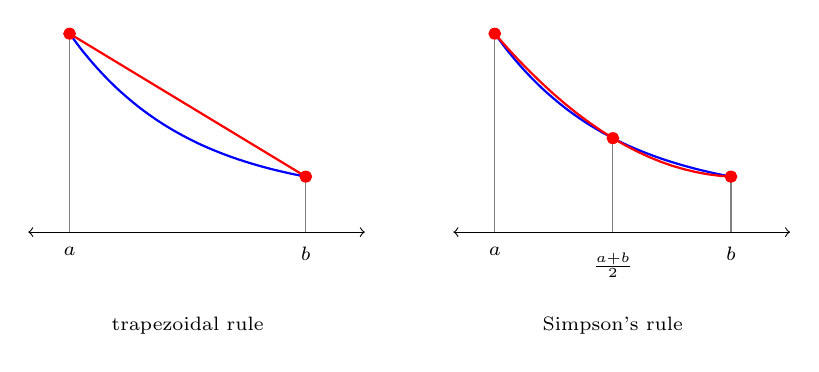
\begin{tikzpicture}[xscale=1.5,yscale=1.4]
  % trapezium
  \begin{scope}
    \draw[<->] (-0.35,0) -- (2.5,0);
    \draw[thick,smooth,color=blue] plot coordinates {(0.000,1.800) (0.100,1.657) (0.200,1.528)
      (0.300,1.411) (0.400,1.305) (0.500,1.210) (0.600,1.123) (0.700,1.045) (0.800,0.974)
      (0.900,0.910) (1.000,0.852) (1.100,0.799) (1.200,0.752) (1.300,0.709) (1.400,0.670)
      (1.500,0.635) (1.600,0.603) (1.700,0.574) (1.800,0.548) (1.900,0.524) (2.000,0.503)};
    \draw[thick,color=red] (0,1.8) -- (2,0.503);
    \draw[thin,color=gray] (0,0) -- (0,1.8);
    \draw[thin,color=gray] (2,0) -- (2,0.503);
    \filldraw[color=red] (0,1.8) circle (1.4pt);
    \filldraw[color=red] (2,0.503) circle (1.4pt);
    \node[below] at (0,-0.05) {\scriptsize $a$};
    \node[below] at (2,-0.05) {\scriptsize $b$};
    \node at (1,-0.85) {\scriptsize trapezoidal rule};
  \end{scope}
  % simpson
  \begin{scope}[xshift=3.6cm]
    \draw[<->] (-0.35,0) -- (2.5,0);
    \draw[thick,smooth,color=blue] plot coordinates {(0.000,1.800) (0.100,1.657) (0.200,1.528)
      (0.300,1.411) (0.400,1.305) (0.500,1.210) (0.600,1.123) (0.700,1.045) (0.800,0.974)
      (0.900,0.910) (1.000,0.852) (1.100,0.799) (1.200,0.752) (1.300,0.709) (1.400,0.670)
      (1.500,0.635) (1.600,0.603) (1.700,0.574) (1.800,0.548) (1.900,0.524) (2.000,0.503)};
    \draw[thick,color=red] plot coordinates {(0.000,1.800) (0.100,1.678) (0.200,1.562)
      (0.300,1.453) (0.400,1.349) (0.500,1.251) (0.600,1.159) (0.700,1.073) (0.800,0.994)
      (0.900,0.920) (1.000,0.852) (1.100,0.790) (1.200,0.734) (1.300,0.684) (1.400,0.640)
      (1.500,0.602) (1.600,0.571) (1.700,0.545) (1.800,0.525) (1.900,0.511) (2.000,0.503)};
    \draw[thin,color=gray] (0,0) -- (0,1.8);
    \draw[thin,color=gray] (1,0) -- (1,0.852);
    \draw[thin,color=gray] (2,0) -- (2,0.503);
    \filldraw[color=red] (0,1.8) circle (1.4pt);
    \filldraw[color=red] (1,0.852) circle (1.4pt);
    \filldraw[color=red] (2,0.503) circle (1.4pt);
    \node[below] at (0,-0.05) {\scriptsize $a$};
    \node[below] at (1,-0.10) {\scriptsize $\frac{a+b}{2}$};
    \node[below] at (2,-0.05) {\scriptsize $b$};
    \node at (1,-0.85) {\scriptsize Simpson's rule};
  \end{scope}
\end{tikzpicture}
\end{center}

\begin{remark}
  One might hope that taking $\nu$ larger and larger gives better and better rules. It does not: for $\nu \geq 8$ some of the weights $a_i$ become negative, and by $\nu = 30$ they are enormous, so that rounding errors are amplified catastrophically. This is the Runge phenomenon again, wearing a different hat. In practice one instead uses a \emph{composite} rule: chop $[a,b]$ into many small subintervals and apply a low-order rule (usually the trapezoidal or Simpson's rule) on each.
\end{remark}

\subsection{Gaussian Quadrature}

Now we use our remaining freedom. We work with a weighted integral
$$
L(f) = \int_a^b w(x)f(x)\dd x,
$$
and seek \vocab{weights} $b_1, \dots, b_\nu$ and \vocab{nodes} $c_1, \dots, c_\nu \in [a,b]$ such that
$$
\int_a^b w(x)f(x)\dd x \approx \sum_{k=1}^{\nu}b_k f(c_k)
$$
is exact for polynomials of as high a degree as possible. (The notation is traditional for this topic and clashes slightly with the rest of the course; we shall live with it.)

First, a limit on our ambitions.

\begin{proposition}\label{prop:gaussmax}
  No choice of $\nu$ nodes and weights gives a formula exact for all $f \in \Pn{2\nu}$.
\end{proposition}
\begin{proof}
  Consider $q(x) = \prod_{k=1}^\nu (x - c_k)$, so that $q^2 \in \Pn{2\nu}$. Then $\sum_k b_k q^2(c_k) = 0$, whereas
  $$
  \int_a^b w(x)q(x)^2\dd x > 0,
  $$
  since $wq^2 \geq 0$ is continuous and not identically zero.
\end{proof}

So $2\nu - 1$ is the best we could possibly hope for, and we shall achieve it. The clue is in the proof: we need the nodes to be the roots of a polynomial that is orthogonal to everything of low degree. Before that, we must check that such roots are usable at all -- they had better be real, distinct, and inside $(a,b)$.

\begin{theorem}[Zeros of Orthogonal Polynomials]\label{thm:oproots}
  For $\nu \geq 1$, the monic orthogonal polynomial $p_\nu$ associated with $\ip{f}{g} = \int_a^b wfg\dd x$ has $\nu$ distinct real zeros, all lying in $(a,b)$.
\end{theorem}
\begin{proof}
  Since $p_0 \equiv 1$ and $\ip{p_\nu}{p_0} = 0$ for $\nu \geq 1$, we have
  $$
  \int_a^b w(x)p_\nu(x)\dd x = 0,
  $$
  and as $w \geq 0$ is not identically zero, $p_\nu$ must change sign somewhere in $(a,b)$.

  Let $\varphi_1, \dots, \varphi_m$ be the points of $(a,b)$ at which $p_\nu$ changes sign; we have just shown $m \geq 1$, and certainly $m \leq \nu$ since these are among the zeros of $p_\nu$. Put
  $$
  q(x) = \prod_{j=1}^{m}(x - \varphi_j) \in \Pn{m}.
  $$
  Then $q$ changes sign at exactly the same points as $p_\nu$, so $qp_\nu$ has constant sign on $(a,b)$ and is not identically zero; hence $\ip{q}{p_\nu} = \int_a^b w q p_\nu \dd x \neq 0$. But $p_\nu$ is orthogonal to every polynomial of degree less than $\nu$, so we must have $m \geq \nu$, and therefore $m = \nu$.

  Thus $p_\nu$ has $\nu$ distinct sign changes in $(a,b)$, which accounts for all $\nu$ of its zeros; they are real, distinct, and lie in $(a,b)$.
\end{proof}

Before choosing the nodes, let us record what the interpolatory choice of weights gives for \emph{any} nodes.

\begin{theorem}[Ordinary Quadrature]\label{thm:ordquad}
  Let $c_1, \dots, c_\nu \in [a,b]$ be distinct, with fundamental Lagrange polynomials $\ell_1, \dots, \ell_\nu$. If we choose
  $$
  b_k = \int_a^b w(x)\ell_k(x)\dd x,
  $$
  then the quadrature formula is exact for all $f \in \Pn{\nu - 1}$.
\end{theorem}
\begin{proof}
  For $f \in \Pn{\nu-1}$, interpolation at $\nu$ points reproduces $f$ exactly, so $f = \sum_k f(c_k)\ell_k$. Integrating against $w$ gives $\int_a^b wf = \sum_k f(c_k) b_k$.
\end{proof}

And now the theorem that makes it all worthwhile.

\begin{theorem}[Gaussian Quadrature]\label{thm:gauss}
  Choose the nodes $c_1, \dots, c_\nu$ to be the zeros of the orthogonal polynomial $p_\nu$, and the weights $b_k$ as in Theorem \ref{thm:ordquad}. Then the quadrature formula
  $$
  \int_a^b w(x)f(x)\dd x \approx \sum_{k=1}^\nu b_k f(c_k)
  $$
  is exact for all $f \in \Pn{2\nu - 1}$. Moreover every weight $b_k$ is strictly positive.
\end{theorem}
\begin{proof}
  Let $f \in \Pn{2\nu-1}$. Dividing by $p_\nu$ we may write
  $$
  f = qp_\nu + r, \qquad q, r \in \Pn{\nu-1}.
  $$
  Since $p_\nu$ is orthogonal to all of $\Pn{\nu-1}$, we have $\int_a^b w q p_\nu \dd x = \ip{q}{p_\nu} = 0$, so
  $$
  \int_a^b w(x)f(x)\dd x = \int_a^b w(x)r(x)\dd x .
  $$
  On the other side, each $c_k$ is a zero of $p_\nu$, so $f(c_k) = r(c_k)$ and hence
  $$
  \sum_{k=1}^\nu b_k f(c_k) = \sum_{k=1}^\nu b_k r(c_k).
  $$
  But $r \in \Pn{\nu - 1}$, so by Theorem \ref{thm:ordquad} the two right-hand sides agree. Hence the formula is exact for $f$.

  For positivity, apply exactness to $f = \ell_k^2 \in \Pn{2\nu-2}$. Then
  $$
  0 < \int_a^b w(x)\ell_k(x)^2 \dd x = \sum_{j=1}^\nu b_j \ell_k(c_j)^2 = \sum_{j=1}^\nu b_j \delta_{jk} = b_k. \qedhere
  $$
\end{proof}

Together with Proposition \ref{prop:gaussmax}, this says that Gaussian quadrature is optimal: $2\nu - 1$ is achieved and $2\nu$ is impossible. The positivity of the weights is not a footnote either -- it is what makes the rule numerically stable, since it means there is no cancellation between the terms and rounding errors cannot be amplified.

For the Legendre weight $w \equiv 1$ on $[-1,1]$ the nodes are the zeros of the Legendre polynomials. Here is $P_4$ with its four zeros marked; these are the nodes of the four-point Gauss--Legendre rule, which is exact for all polynomials of degree up to $7$.
\begin{center}
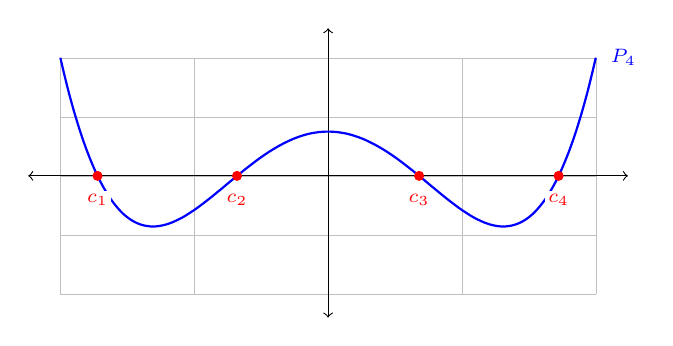
\begin{tikzpicture}
  \draw[ultra thin,color=lightgray] (-3.400,-1.500) -- (-3.400,1.500);
  \draw[ultra thin,color=lightgray] (-1.700,-1.500) -- (-1.700,1.500);
  \draw[ultra thin,color=lightgray] (0.000,-1.500) -- (0.000,1.500);
  \draw[ultra thin,color=lightgray] (1.700,-1.500) -- (1.700,1.500);
  \draw[ultra thin,color=lightgray] (3.400,-1.500) -- (3.400,1.500);
  \draw[ultra thin,color=lightgray] (-3.400,-1.500) -- (3.400,-1.500);
  \draw[ultra thin,color=lightgray] (-3.400,-0.750) -- (3.400,-0.750);
  \draw[ultra thin,color=lightgray] (-3.400,0.000) -- (3.400,0.000);
  \draw[ultra thin,color=lightgray] (-3.400,0.750) -- (3.400,0.750);
  \draw[ultra thin,color=lightgray] (-3.400,1.500) -- (3.400,1.500);
  \draw[<->] (-3.808,0) -- (3.808,0);
  \draw[<->] (0,-1.800) -- (0,1.875);
  \draw[thick,smooth,color=blue] plot coordinates {
    (-3.400,1.500) (-3.343,1.259) (-3.287,1.037) (-3.230,0.831) (-3.173,0.642) (-3.117,0.470)
    (-3.060,0.312) (-3.003,0.169) (-2.947,0.040) (-2.890,-0.076) (-2.833,-0.179) (-2.777,-0.270)
    (-2.720,-0.349) (-2.663,-0.418) (-2.607,-0.477) (-2.550,-0.525) (-2.493,-0.565)
    (-2.437,-0.595) (-2.380,-0.618) (-2.323,-0.633) (-2.267,-0.641) (-2.210,-0.643)
    (-2.153,-0.638) (-2.097,-0.628) (-2.040,-0.612) (-1.983,-0.592) (-1.927,-0.567)
    (-1.870,-0.539) (-1.813,-0.507) (-1.757,-0.471) (-1.700,-0.434) (-1.643,-0.393)
    (-1.587,-0.351) (-1.530,-0.307) (-1.473,-0.262) (-1.417,-0.216) (-1.360,-0.170)
    (-1.303,-0.122) (-1.247,-0.075) (-1.190,-0.028) (-1.133,0.019) (-1.077,0.064) (-1.020,0.109)
    (-0.963,0.153) (-0.907,0.196) (-0.850,0.237) (-0.793,0.276) (-0.737,0.313) (-0.680,0.348)
    (-0.623,0.381) (-0.567,0.411) (-0.510,0.439) (-0.453,0.465) (-0.397,0.487) (-0.340,0.507)
    (-0.283,0.524) (-0.227,0.538) (-0.170,0.548) (-0.113,0.556) (-0.057,0.561) (0.000,0.562)
    (0.057,0.561) (0.113,0.556) (0.170,0.548) (0.227,0.538) (0.283,0.524) (0.340,0.507)
    (0.397,0.487) (0.453,0.465) (0.510,0.439) (0.567,0.411) (0.623,0.381) (0.680,0.348)
    (0.737,0.313) (0.793,0.276) (0.850,0.237) (0.907,0.196) (0.963,0.153) (1.020,0.109)
    (1.077,0.064) (1.133,0.019) (1.190,-0.028) (1.247,-0.075) (1.303,-0.122) (1.360,-0.169)
    (1.417,-0.216) (1.473,-0.262) (1.530,-0.307) (1.587,-0.351) (1.643,-0.393) (1.700,-0.434)
    (1.757,-0.471) (1.813,-0.507) (1.870,-0.539) (1.927,-0.567) (1.983,-0.592) (2.040,-0.612)
    (2.097,-0.628) (2.153,-0.638) (2.210,-0.643) (2.267,-0.641) (2.323,-0.633) (2.380,-0.618)
    (2.437,-0.595) (2.493,-0.565) (2.550,-0.525) (2.607,-0.477) (2.663,-0.418) (2.720,-0.349)
    (2.777,-0.270) (2.833,-0.179) (2.890,-0.076) (2.947,0.040) (3.003,0.169) (3.060,0.312)
    (3.117,0.470) (3.173,0.642) (3.230,0.831) (3.287,1.037) (3.343,1.259) (3.400,1.500)
  };
  \filldraw[color=red] (-2.928,0.000) circle (1.6pt);
  \filldraw[color=red] (-1.156,0.000) circle (1.6pt);
  \filldraw[color=red] (1.156,0.000) circle (1.6pt);
  \filldraw[color=red] (2.928,0.000) circle (1.6pt);
  \node[below,color=red,fill=white,inner sep=1.2pt] at (-2.928,-0.180) {\scriptsize $c_1$};
  \node[below,color=red,fill=white,inner sep=1.2pt] at (-1.156,-0.180) {\scriptsize $c_2$};
  \node[below,color=red,fill=white,inner sep=1.2pt] at (1.156,-0.180) {\scriptsize $c_3$};
  \node[below,color=red,fill=white,inner sep=1.2pt] at (2.928,-0.180) {\scriptsize $c_4$};
  \node[color=blue,right] at (3.468,1.500) {\scriptsize $P_4$};
\end{tikzpicture}
\end{center}

\begin{example}[Gauss--Legendre Rules]
  For $w \equiv 1$ on $[-1,1]$ the first few rules are as follows.
  \begin{center}
    \begin{tabular}{clll}
      \toprule
      $\nu$ & nodes $c_k$ & weights $b_k$ & exact on\\
      \midrule
      $1$ & $0$ & $2$ & $\Pn{1}$\\
      $2$ & $\pm 1/\sqrt3$ & $1,\ 1$ & $\Pn{3}$\\
      $3$ & $0,\ \pm\sqrt{3/5}$ & $8/9,\ 5/9,\ 5/9$ & $\Pn{5}$\\
      $4$ & $\pm 0.3399810$, $\pm 0.8611363$ & $0.6521452$, $0.3478548$ & $\Pn{7}$\\
      \bottomrule
    \end{tabular}
  \end{center}
  Let us check the case $\nu = 2$ directly. The nodes are the zeros of $p_2 = x^2 - \tfrac13$, namely $\pm 1/\sqrt3$. The rule $\int_{-1}^1 f \approx f(-1/\sqrt3) + f(1/\sqrt3)$ certainly integrates $1$ and $x$ correctly. For $x^2$ it gives $2/3$, which is right; for $x^3$ it gives $0$, which is right. And for $x^4$ it gives $2/9$ against the true value $2/5$ -- so exactness stops at degree $3 = 2\nu -1$, exactly as predicted.
\end{example}

\begin{example}[Gauss Beats Simpson]
  Let us approximate $\int_0^1 e^x \dd x = e - 1 = 1.718282$. Substituting $x = (t+1)/2$ turns this into $\tfrac12\int_{-1}^1 e^{(t+1)/2}\dd t$, and the two-point Gauss rule gives
  $$
  \tfrac12\left(e^{(1 - 1/\sqrt3)/2} + e^{(1+1/\sqrt3)/2}\right) = \tfrac12(1.235345 + 2.200455) = 1.717900,
  $$
  an error of $3.8 \times 10^{-4}$, using \emph{two} evaluations of $f$. Simpson's rule, using \emph{three} evaluations, gives
  $$
  \tfrac16\left(1 + 4e^{1/2} + e\right) = 1.718861,
  $$
  an error of $5.8\times 10^{-4}$. The trapezoidal rule gives $1.859141$, an error of $0.14$. Gaussian quadrature does more with less.
\end{example}

\begin{remark}
  The price of Gaussian quadrature is that the nodes are irrational and must be looked up or computed (they are eigenvalues of the tridiagonal matrix formed from the three-term recurrence coefficients, which is how one actually computes them). Also, unlike a composite Newton--Cotes rule, refining from $\nu$ to $\nu+1$ points reuses none of the old function evaluations. Both objections are real, and both have been engineered around; but the exactness result of Theorem \ref{thm:gauss} is why Gaussian quadrature remains the default for smooth integrands.
\end{remark}


\section{Expressing Errors in Terms of Derivatives}

We now have a supply of approximations to linear functionals, each of them exact on some space $\Pn{k}$ of polynomials. What we do not yet have is a systematic way to say how large the error is when $f$ is \emph{not} a polynomial. The Peano kernel theorem provides exactly that: it converts the statement `the error annihilates $\Pn{k}$' into an exact integral formula for the error in terms of $f^{(k+1)}$.

The setup is as follows. We have a linear functional $L$, an approximation $\sum_{i=0}^n a_i L_i(f)$ built from simpler functionals $L_i$, and the error functional
$$
e_L(f) = L(f) - \sum_{i=0}^{n}a_i L_i(f),
$$
which is again linear. We suppose that $e_L(f) = 0$ for all $f \in \Pn{k}$; we say that $e_L$ \vocab{annihilates} $\Pn{k}$.

\begin{example}
  Suppose we approximate $L(f) = f(\beta)$ by the (rather silly) formula
  $$
  L(f) \approx f(\alpha) + \frac{\beta - \alpha}{2}\big(f'(\alpha) + f'(\beta)\big), \qquad \alpha \neq \beta.
  $$
  Then
  $$
  e_L(f) = f(\beta) - f(\alpha) - \frac{\beta-\alpha}{2}\big(f'(\alpha) + f'(\beta)\big).
  $$
  One checks directly that this vanishes for $f = 1, x, x^2$: for $f = x^2$, the left-hand piece is $\beta^2 - \alpha^2$ and the right-hand piece is $(\beta-\alpha)(\alpha+\beta)$, which agree. It does not vanish for $f = x^3$. So $e_L$ annihilates $\Pn{2}$.
\end{example}

We want a bound of the form
$$
\abs{e_L(f)} \leq c_L \norm{f^{(k+1)}}_\infty,
$$
with $c_L$ as small as possible. For this we need $[a,b]$ to be finite, so that the suprema exist.

\begin{definition}[Sharp Constant]
  The constant $c_L$ is \vocab{sharp} if for every $\varepsilon > 0$ there is some $f_\varepsilon \in C^{k+1}[a,b]$ with
  $$
  \abs{e_L(f_\varepsilon)} \geq (c_L - \varepsilon)\norm{f_\varepsilon^{(k+1)}}_\infty .
  $$
\end{definition}

\subsection{The Peano Kernel Theorem}

The tool is Taylor's theorem with integral remainder,
$$
f(x) = f(a) + (x-a)f'(a) + \cdots + \frac{(x-a)^k}{k!}f^{(k)}(a) + \frac{1}{k!}\int_a^x (x-\theta)^k f^{(k+1)}(\theta)\dd\theta .
$$
The awkwardness is that $x$ appears in the limit of the integral, which stops us from interchanging $e_L$ with $\int$. We fix this with a piece of notation.

\begin{definition}[Truncated Power Function]
  For $k \geq 0$ we define
  $$
  (x - \theta)_+^k = \begin{cases} (x-\theta)^k & x \geq \theta,\\ 0 & x < \theta.\end{cases}
  $$
\end{definition}

Note that for $k \geq 1$ this is a $C^{k-1}$ function of $x$: it is smooth except at $x = \theta$, where the first $k-1$ derivatives all vanish from both sides. With it, the Taylor remainder becomes
$$
\frac{1}{k!}\int_a^b (x-\theta)_+^k f^{(k+1)}(\theta)\dd\theta,
$$
where now the limits do not involve $x$.

\begin{theorem}[Peano Kernel Theorem]\label{thm:peano}
  Let $[a,b]$ be finite and let $e_L$ be a linear functional annihilating $\Pn{k}$ which commutes with the integral in the sense below. Then for all $f \in C^{k+1}[a,b]$,
  $$
  e_L(f) = \frac{1}{k!}\int_a^b K(\theta) f^{(k+1)}(\theta)\dd\theta, \qquad K(\theta) = e_L\big((x-\theta)_+^k\big),
  $$
  where $e_L$ acts on $(x-\theta)_+^k$ as a function of $x$, with $\theta$ held fixed.
\end{theorem}
\begin{proof}
  Write $f = T + R$ where $T \in \Pn{k}$ is the Taylor polynomial of $f$ about $a$ of degree $k$ and
  $$
  R(x) = \frac{1}{k!}\int_a^b (x-\theta)_+^k f^{(k+1)}(\theta)\dd\theta
  $$
  is the remainder. Since $e_L$ annihilates $\Pn{k}$ we have $e_L(T) = 0$, so by linearity $e_L(f) = e_L(R)$. Interchanging $e_L$ with the integral,
  $$
  e_L(f) = \frac{1}{k!}\int_a^b e_L\big((x-\theta)_+^k\big)f^{(k+1)}(\theta)\dd\theta = \frac{1}{k!}\int_a^b K(\theta)f^{(k+1)}(\theta)\dd\theta. \qedhere
  $$
\end{proof}

\begin{remark}
  The interchange of $e_L$ with the integral is the only step needing care. For the functionals we use in this course -- point values, point values of derivatives, and integrals, together with finite linear combinations of these -- the interchange is valid and can be verified directly in each case (for integrals it is Fubini, for point evaluations it is trivial, and for derivatives one differentiates under the integral sign). A sufficiently determined pure mathematician can construct linear functionals for which it fails, but we shall not meet any.
\end{remark}

The point of the theorem is that $K$ depends only on $L$ and not at all on $f$. So having computed $K$ once, we get a whole family of bounds by applying Hölder's inequality in different ways:
$$
\abs{e_L(f)} \leq \frac{1}{k!}\begin{cases}
\displaystyle \left(\int_a^b\abs{K(\theta)}\dd\theta\right)\norm{f^{(k+1)}}_\infty,\\[2ex]
\displaystyle \left(\int_a^b \abs{K(\theta)}^2\dd\theta\right)^{1/2}\norm{f^{(k+1)}}_2,\\[2ex]
\displaystyle \norm{K}_\infty \norm{f^{(k+1)}}_1 .
\end{cases}
$$
These constants can be shown to be sharp. And do not forget the factor $1/k!$ when computing $c_L$ -- it is the most commonly dropped piece of the whole formula.

There is one very common situation in which we can say considerably more.

\begin{proposition}[Sign-Definite Kernels]\label{prop:signdef}
  If $K$ does not change sign on $[a,b]$, then for every $f \in C^{k+1}[a,b]$ there is some $\xi \in (a,b)$, depending on $f$, with
  $$
  e_L(f) = \frac{1}{k!}\left(\int_a^b K(\theta)\dd\theta\right)f^{(k+1)}(\xi).
  $$
  Moreover the constant $c_L = \frac{1}{k!}\abs{\int_a^b K}$ in the $\norm{\cdot}_\infty$ bound is attained, by $f(x) = x^{k+1}$.
\end{proposition}
\begin{proof}
  Since $K$ has constant sign, the integral mean value theorem applies to $\int_a^b K f^{(k+1)}$ and yields $f^{(k+1)}(\xi)\int_a^b K$ for some $\xi$. For the second statement, $f = x^{k+1}$ has $f^{(k+1)} \equiv (k+1)!$ constant, so the inequality $\abs{\int K f^{(k+1)}}\le \int\abs{K}\cdot\norm{f^{(k+1)}}_\infty$ is an equality.
\end{proof}

\subsection{Worked Kernels}

Peano kernels are computed by brute force: substitute $(x-\theta)_+^k$ into the formula for $e_L$, and remember that the truncated power vanishes when its argument is negative, so the answer is piecewise.

\begin{example}[The Trapezoidal Rule]\label{eg:trapkernel}
  Take $[a,b] = [0,1]$ and
  $$
  e_L(f) = \int_0^1 f(x)\dd x - \tfrac12\big(f(0) + f(1)\big),
  $$
  which annihilates $\Pn{1}$, so $k = 1$. Then for $\theta \in [0,1]$,
  $$
  K(\theta) = \int_0^1 (x-\theta)_+\dd x - \tfrac12\big((0-\theta)_+ + (1-\theta)_+\big) = \int_\theta^1 (x - \theta)\dd x - \tfrac12(1-\theta),
  $$
  since $(0-\theta)_+ = 0$ for $\theta \geq 0$. Hence
  $$
  K(\theta) = \frac{(1-\theta)^2}{2} - \frac{1-\theta}{2} = -\frac{\theta(1-\theta)}{2}.
  $$
  This is a downward parabola vanishing at both endpoints, so $K \leq 0$ throughout and Proposition \ref{prop:signdef} applies. We have $\int_0^1 K = -\tfrac12(\tfrac12 - \tfrac13) = -\tfrac1{12}$, so
  $$
  e_L(f) = -\tfrac{1}{12}f''(\xi), \qquad \abs{e_L(f)} \leq \tfrac{1}{12}\norm{f''}_\infty,
  $$
  which is the classical trapezoidal rule error, now derived rather than conjured.
\end{example}

\begin{example}[Simpson's Rule]\label{eg:simpsonkernel}
  Take $[a,b] = [-1,1]$ and
  $$
  e_L(f) = \int_{-1}^1 f(x)\dd x - \tfrac13\big(f(-1) + 4f(0) + f(1)\big).
  $$
  We saw that this annihilates $\Pn{3}$, so we may take $k = 3$. For $\theta \in [0,1]$ only the $f(1)$ term survives the truncation, and
  $$
  K(\theta) = \int_\theta^1 (x-\theta)^3\dd x - \tfrac13(1-\theta)^3 = \frac{(1-\theta)^4}{4} - \frac{(1-\theta)^3}{3}.
  $$
  For $\theta \in [-1,0]$ the $f(0)$ term also contributes, giving
  $$
  K(\theta) = \frac{(1-\theta)^4}{4} - \frac{1}{3}\left(4(-\theta)^3 + (1-\theta)^3\right).
  $$
  One checks that the two branches agree at $\theta = 0$, both giving $\tfrac14 - \tfrac13 = -\tfrac1{12}$, and that $K(\pm 1) = 0$. In fact $K$ is symmetric, $K(-\theta) = K(\theta)$, and negative on $(-1,1)$.
\end{example}

Here is the kernel of Example \ref{eg:simpsonkernel}, plotted on $[-1,1]$.
\begin{center}
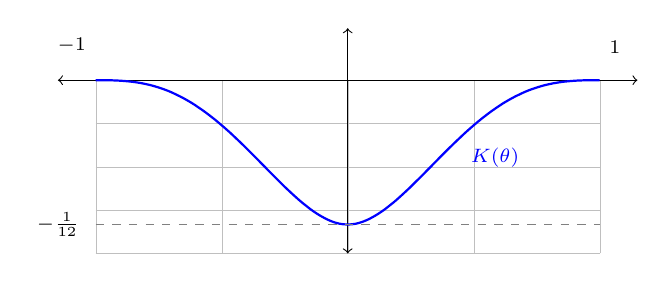
\begin{tikzpicture}
  \draw[ultra thin,color=lightgray] (-3.200,-2.200) -- (-3.200,0.000);
  \draw[ultra thin,color=lightgray] (-1.600,-2.200) -- (-1.600,0.000);
  \draw[ultra thin,color=lightgray] (0.000,-2.200) -- (0.000,0.000);
  \draw[ultra thin,color=lightgray] (1.600,-2.200) -- (1.600,0.000);
  \draw[ultra thin,color=lightgray] (3.200,-2.200) -- (3.200,0.000);
  \draw[ultra thin,color=lightgray] (-3.200,-2.200) -- (3.200,-2.200);
  \draw[ultra thin,color=lightgray] (-3.200,-1.650) -- (3.200,-1.650);
  \draw[ultra thin,color=lightgray] (-3.200,-1.100) -- (3.200,-1.100);
  \draw[ultra thin,color=lightgray] (-3.200,-0.550) -- (3.200,-0.550);
  \draw[ultra thin,color=lightgray] (-3.200,-0.000) -- (3.200,-0.000);
  \draw[<->] (-3.680,0) -- (3.680,0);
  \draw[<->] (0,-2.200) -- (0,0.660);
  \draw[thick,smooth,color=blue] plot coordinates {
    (-3.200,0.000) (-3.147,-0.000) (-3.093,-0.000) (-3.040,-0.001) (-2.987,-0.002)
    (-2.933,-0.004) (-2.880,-0.007) (-2.827,-0.011) (-2.773,-0.016) (-2.720,-0.022)
    (-2.667,-0.030) (-2.613,-0.039) (-2.560,-0.050) (-2.507,-0.062) (-2.453,-0.077)
    (-2.400,-0.093) (-2.347,-0.111) (-2.293,-0.131) (-2.240,-0.153) (-2.187,-0.178)
    (-2.133,-0.204) (-2.080,-0.232) (-2.027,-0.262) (-1.973,-0.294) (-1.920,-0.329)
    (-1.867,-0.365) (-1.813,-0.403) (-1.760,-0.443) (-1.707,-0.484) (-1.653,-0.528)
    (-1.600,-0.573) (-1.547,-0.619) (-1.493,-0.667) (-1.440,-0.717) (-1.387,-0.767)
    (-1.333,-0.819) (-1.280,-0.871) (-1.227,-0.924) (-1.173,-0.978) (-1.120,-1.032)
    (-1.067,-1.086) (-1.013,-1.141) (-0.960,-1.195) (-0.907,-1.248) (-0.853,-1.301)
    (-0.800,-1.354) (-0.747,-1.404) (-0.693,-1.454) (-0.640,-1.502) (-0.587,-1.548)
    (-0.533,-1.591) (-0.480,-1.633) (-0.427,-1.671) (-0.373,-1.706) (-0.320,-1.737)
    (-0.267,-1.765) (-0.213,-1.789) (-0.160,-1.808) (-0.107,-1.822) (-0.053,-1.830)
    (0.000,-1.833) (0.053,-1.830) (0.107,-1.822) (0.160,-1.808) (0.213,-1.789) (0.267,-1.765)
    (0.320,-1.737) (0.373,-1.706) (0.427,-1.671) (0.480,-1.633) (0.533,-1.591) (0.587,-1.548)
    (0.640,-1.502) (0.693,-1.454) (0.747,-1.404) (0.800,-1.354) (0.853,-1.301) (0.907,-1.248)
    (0.960,-1.195) (1.013,-1.141) (1.067,-1.086) (1.120,-1.032) (1.173,-0.978) (1.227,-0.924)
    (1.280,-0.871) (1.333,-0.819) (1.387,-0.767) (1.440,-0.717) (1.493,-0.667) (1.547,-0.619)
    (1.600,-0.573) (1.653,-0.528) (1.707,-0.484) (1.760,-0.443) (1.813,-0.403) (1.867,-0.365)
    (1.920,-0.329) (1.973,-0.294) (2.027,-0.262) (2.080,-0.232) (2.133,-0.204) (2.187,-0.178)
    (2.240,-0.153) (2.293,-0.131) (2.347,-0.111) (2.400,-0.093) (2.453,-0.077) (2.507,-0.062)
    (2.560,-0.050) (2.613,-0.039) (2.667,-0.030) (2.720,-0.022) (2.773,-0.016) (2.827,-0.011)
    (2.880,-0.007) (2.933,-0.004) (2.987,-0.002) (3.040,-0.001) (3.093,-0.000) (3.147,-0.000)
    (3.200,0.000)
  };
  \node[above left] at (-3.200,0.220) {\scriptsize $-1$};
  \node[above right] at (3.200,0.220) {\scriptsize $1$};
  \draw[thin,dashed,color=gray] (-3.200,-1.833) -- (3.200,-1.833);
  \node[left] at (-3.28,-1.833) {\scriptsize $-\frac{1}{12}$};
  \node[color=blue,right] at (1.440,-0.990) {\scriptsize $K(\theta)$};
\end{tikzpicture}
\end{center}

Since $K \le 0$ we may use Proposition \ref{prop:signdef}. Computing the integral,
$$
\int_{-1}^{1}K(\theta)\dd\theta = 2\int_0^1\left(\frac{(1-\theta)^4}{4} - \frac{(1-\theta)^3}{3}\right)\dd\theta = 2\left(\frac{1}{20} - \frac{1}{12}\right) = -\frac{1}{15},
$$
and hence, with $k = 3$ so that $1/k! = 1/6$,
$$
e_L(f) = -\frac{1}{90}f^{(4)}(\xi), \qquad \abs{e_L(f)} \leq \frac{1}{90}\norm{f^{(4)}}_\infty
$$
for some $\xi \in (-1,1)$. Rescaling to a general interval gives the familiar $-\frac{(b-a)^5}{2880}f^{(4)}(\xi)$.

The theorem applies just as well to functionals that have nothing to do with integration.

\begin{example}[A Derivative Formula]
  Suppose we approximate $f'(0)$ by the one-sided formula
  $$
  f'(0) \approx -\tfrac32 f(0) + 2f(1) - \tfrac12 f(2),
  $$
  so that $e_L(f) = f'(0) + \tfrac32 f(0) - 2f(1) + \tfrac12 f(2)$ on $[0,2]$. Checking on $1, x, x^2$: for $f = 1$ we get $0 + \tfrac32 - 2 + \tfrac12 = 0$; for $f = x$ we get $1 + 0 - 2 + 1 = 0$; for $f = x^2$ we get $0 + 0 - 2 + 2 = 0$. For $f = x^3$ we get $0 + 0 - 2 + 4 = 2 \neq 0$. So $e_L$ annihilates $\Pn{2}$ and $k = 2$.

  The kernel is $K(\theta) = e_L\big((x-\theta)_+^2\big)$. Since $\tfrac{\dd}{\dd x}(x-\theta)_+^2 = 2(x-\theta)_+$, the derivative term contributes $2(0-\theta)_+ = 0$ for $\theta \ge 0$, as does the $f(0)$ term. So
  $$
  K(\theta) = -2(1-\theta)_+^2 + \tfrac12(2-\theta)_+^2 = \begin{cases} 2\theta - \tfrac32\theta^2, & \theta \in [0,1],\\[1ex] \tfrac12(2-\theta)^2, & \theta \in [1,2].\end{cases}
  $$
  (The two branches agree at $\theta = 1$, both giving $\tfrac12$.) Both branches are non-negative, so $K \geq 0$ and Proposition \ref{prop:signdef} applies. We have
  $$
  \int_0^2 K(\theta)\dd\theta = \int_0^1\left(2\theta - \tfrac32\theta^2\right)\dd\theta + \int_1^2 \tfrac12(2-\theta)^2\dd\theta = \tfrac12 + \tfrac16 = \tfrac23,
  $$
  and hence, remembering the factor $1/k! = 1/2$,
  $$
  e_L(f) = \tfrac13 f'''(\xi), \qquad \abs{e_L(f)} \leq \tfrac13\norm{f'''}_\infty
  $$
  for some $\xi \in (0,2)$.
\end{example}

\begin{remark}
  A final subtlety. If $e_L$ annihilates $\Pn{k}$ then it also annihilates $\Pn{j}$ for every $j < k$, so we get a \emph{different} kernel $K_j(\theta) = e_L((x-\theta)_+^j)$ and a different error formula
  $$
  e_L(f) = \frac{1}{j!}\int_a^b K_j(\theta)f^{(j+1)}(\theta)\dd\theta
  $$
  valid for $f \in C^{j+1}[a,b]$. Usually taking $j = k$ is best, as it extracts the most information. But if $f$ happens to be only $C^{j+1}$ and not $C^{k+1}$ -- and integrands with limited smoothness are common in practice -- then the lower-order kernel is the one that applies. Simpson's rule with a merely twice-differentiable integrand is a case in point.
\end{remark}


\section{Ordinary Differential Equations}

We now turn to what is probably the most important application of numerical analysis. We wish to approximate the solution $y: [0, \infty) \to \R^N$ of the initial value problem
$$
y' = f(t, y), \qquad y(0) = y_0,
$$
where $f: \R \times \R^N \to \R^N$. Note that we allow $y$ to be vector-valued, which costs us nothing notationally and buys us all higher-order scalar equations, since $y'' = g(t,y,y')$ becomes a first-order system in $(y, y')$.

We shall always assume that $f$ is nice enough for the problem to make sense. In particular, we assume $f$ is Lipschitz in its second argument, which by the Picard--Lindelöf theorem guarantees that a unique solution exists; and where we Taylor expand, we assume as much smoothness as the expansion requires. This is standard practice and is not usually where the interesting difficulties lie.

The idea is to replace the continuum of values $y(t)$ by a discrete sequence $y_0, y_1, y_2, \dots$ with $y_n \approx y(t_n)$, where $0 = t_0 < t_1 < \cdots$. We shall almost always take a constant step size, $t_n = nh$. The two questions we must ask of any such scheme are: does $y_n$ actually approach $y(t_n)$ as $h \to 0$, and how fast?

\subsection{One-Step Methods}

\begin{definition}[One-Step Method]
  A \vocab{one-step method} is a recurrence of the form
  $$
  y_{n+1} = \varphi_h(t_n, y_n),
  $$
  in which $y_{n+1}$ depends only on $t_n$, $y_n$, $h$ and $f$.
\end{definition}

The simplest of all is obtained by truncating the Taylor series of $y$ after one term.

\begin{definition}[Euler's Method]
  \vocab{Euler's method} is the one-step method
  $$
  y_{n+1} = y_n + hf(t_n, y_n).
  $$
\end{definition}

The idea is transparent: from the point $(t_n, y_n)$, the differential equation tells us the slope of the solution curve through that point, so we follow that straight line for a time $h$ and see where we end up. The resulting approximation is a polygon, and each segment of it is tangent to \emph{some} solution curve of the equation -- just not, in general, the one we want.

Here is Euler's method applied to $y' = y$, $y(0) = 1$, with $h = 1/4$. The true solution $y(t) = e^t$ is in blue and the Euler polygon in red.
\begin{center}
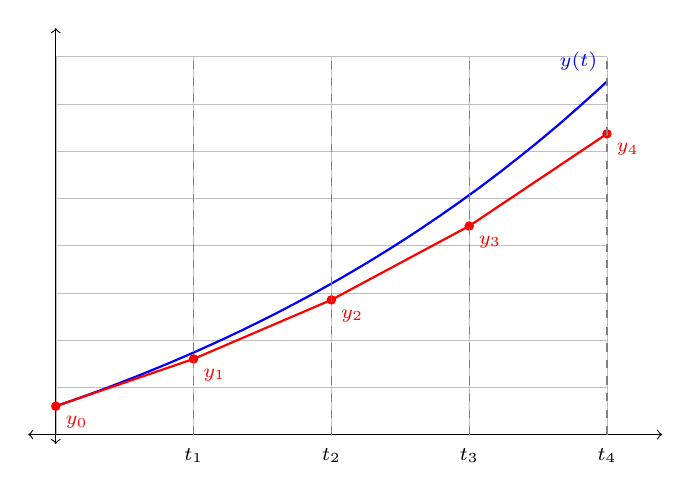
\begin{tikzpicture}
  \draw[ultra thin,color=lightgray] (0.000,2.040) -- (0.000,6.840);
  \draw[ultra thin,color=lightgray] (1.750,2.040) -- (1.750,6.840);
  \draw[ultra thin,color=lightgray] (3.500,2.040) -- (3.500,6.840);
  \draw[ultra thin,color=lightgray] (5.250,2.040) -- (5.250,6.840);
  \draw[ultra thin,color=lightgray] (7.000,2.040) -- (7.000,6.840);
  \draw[ultra thin,color=lightgray] (0.000,2.040) -- (7.000,2.040);
  \draw[ultra thin,color=lightgray] (0.000,2.640) -- (7.000,2.640);
  \draw[ultra thin,color=lightgray] (0.000,3.240) -- (7.000,3.240);
  \draw[ultra thin,color=lightgray] (0.000,3.840) -- (7.000,3.840);
  \draw[ultra thin,color=lightgray] (0.000,4.440) -- (7.000,4.440);
  \draw[ultra thin,color=lightgray] (0.000,5.040) -- (7.000,5.040);
  \draw[ultra thin,color=lightgray] (0.000,5.640) -- (7.000,5.640);
  \draw[ultra thin,color=lightgray] (0.000,6.240) -- (7.000,6.240);
  \draw[ultra thin,color=lightgray] (0.000,6.840) -- (7.000,6.840);
  \draw[<->] (-0.350,2.040) -- (7.700,2.040);
  \draw[<->] (0,1.920) -- (0,7.200);
  \draw[thick,smooth,color=blue] plot coordinates {
    (0.000,2.400) (0.088,2.430) (0.175,2.461) (0.263,2.492) (0.350,2.523) (0.438,2.555)
    (0.525,2.587) (0.613,2.619) (0.700,2.652) (0.787,2.686) (0.875,2.720) (0.963,2.754)
    (1.050,2.788) (1.137,2.823) (1.225,2.859) (1.312,2.895) (1.400,2.931) (1.488,2.968)
    (1.575,3.006) (1.663,3.043) (1.750,3.082) (1.838,3.120) (1.925,3.160) (2.013,3.199)
    (2.100,3.240) (2.188,3.280) (2.275,3.322) (2.363,3.363) (2.450,3.406) (2.538,3.449)
    (2.625,3.492) (2.712,3.536) (2.800,3.580) (2.888,3.625) (2.975,3.671) (3.062,3.717)
    (3.150,3.764) (3.238,3.811) (3.325,3.859) (3.413,3.908) (3.500,3.957) (3.588,4.007)
    (3.675,4.057) (3.762,4.108) (3.850,4.160) (3.938,4.212) (4.025,4.265) (4.112,4.319)
    (4.200,4.373) (4.288,4.428) (4.375,4.484) (4.463,4.540) (4.550,4.597) (4.638,4.655)
    (4.725,4.714) (4.812,4.773) (4.900,4.833) (4.987,4.894) (5.075,4.955) (5.163,5.018)
    (5.250,5.081) (5.338,5.145) (5.425,5.209) (5.513,5.275) (5.600,5.341) (5.688,5.408)
    (5.775,5.477) (5.862,5.545) (5.950,5.615) (6.038,5.686) (6.125,5.757) (6.213,5.830)
    (6.300,5.903) (6.388,5.977) (6.475,6.052) (6.562,6.129) (6.650,6.206) (6.737,6.284)
    (6.825,6.363) (6.913,6.443) (7.000,6.524)
  };
  \draw[thick,color=red] plot coordinates {(0.000,2.400) (1.750,3.000) (3.500,3.750) (5.250,4.688) (7.000,5.859)};
  \filldraw[color=red] (0.000,2.400) circle (1.5pt);
  \filldraw[color=red] (1.750,3.000) circle (1.5pt);
  \filldraw[color=red] (3.500,3.750) circle (1.5pt);
  \filldraw[color=red] (5.250,4.688) circle (1.5pt);
  \filldraw[color=red] (7.000,5.859) circle (1.5pt);
  \node[below right,color=red] at (0.000,2.400) {\scriptsize $y_0$};
  \node[below right,color=red] at (1.750,3.000) {\scriptsize $y_1$};
  \node[below right,color=red] at (3.500,3.750) {\scriptsize $y_2$};
  \node[below right,color=red] at (5.250,4.688) {\scriptsize $y_3$};
  \node[below right,color=red] at (7.000,5.859) {\scriptsize $y_4$};
  \draw[thin,dashed,color=gray] (1.750,2.040) -- (1.750,6.840);
  \draw[thin,dashed,color=gray] (3.500,2.040) -- (3.500,6.840);
  \draw[thin,dashed,color=gray] (5.250,2.040) -- (5.250,6.840);
  \draw[thin,dashed,color=gray] (7.000,2.040) -- (7.000,6.840);
  \node[below] at (1.750,1.992) {\scriptsize $t_1$};
  \node[below] at (3.500,1.992) {\scriptsize $t_2$};
  \node[below] at (5.250,1.992) {\scriptsize $t_3$};
  \node[below] at (7.000,1.992) {\scriptsize $t_4$};
  \node[color=blue,above left] at (7.000,6.523) {\scriptsize $y(t)$};
\end{tikzpicture}
\end{center}

Two things are visible in the picture. The Euler solution lags behind the true one, and the gap grows. What we need to know is whether the gap shrinks to nothing as we shrink $h$.

\begin{definition}[Convergence]
  A method is \vocab{convergent} if, for every $t^* > 0$ and every initial value problem with sufficiently nice $f$,
  $$
  \lim_{h \to 0}\ \max_{n = 0, 1, \dots, \lfloor t^*/h\rfloor} \norm{y_n - y(t_n)} = 0,
  $$
  where $y_n$ is the numerical solution computed with step size $h$.
\end{definition}

Note what this is asking: not that a fixed number of steps become accurate, but that the error at a fixed \emph{time} $t^*$, reached in $\lfloor t^*/h\rfloor$ steps, goes to zero. Since the number of steps grows like $1/h$, the errors made at each step must not be allowed to accumulate too badly. This is the whole content of the following theorem.

\begin{theorem}[Convergence of Euler's Method]\label{thm:eulerconv}
  Suppose $f$ is Lipschitz in its second argument on $[0,t^*] \times \R^N$, that is, there is $\lambda \geq 0$ with
  $$
  \norm{f(t,v) - f(t,w)} \leq \lambda \norm{v - w}
  $$
  for all $t \in [0,t^*]$ and $v, w \in \R^N$. Then Euler's method converges, and indeed the error is $\mathcal{O}(h)$ uniformly on $[0,t^*]$.
\end{theorem}
\begin{proof}
  The Lipschitz condition guarantees by Picard--Lindel\"of that a unique solution $y$ exists on $[0, t^*]$, so the statement makes sense. Write $e_n = y_n - y(t_n)$ for the (global) error at step $n$, and note $e_0 = 0$.

  Taylor's theorem gives $y(t_{n+1}) = y(t_n) + hy'(t_n) + \mathcal{O}(h^2) = y(t_n) + hf(t_n, y(t_n)) + \mathcal{O}(h^2)$, where the $\mathcal{O}(h^2)$ is uniform in $n$ because $y''$ is continuous on the compact interval $[0,t^*]$. Subtracting this from the Euler step,
  \begin{align*}
    \norm{e_{n+1}} &= \norm{y_n + hf(t_n,y_n) - y(t_n) - hf(t_n, y(t_n)) - \mathcal{O}(h^2)}\\
    &\leq \norm{e_n} + h\norm{f(t_n,y_n) - f(t_n,y(t_n))} + ch^2\\
    &\leq (1 + h\lambda)\norm{e_n} + ch^2
  \end{align*}
  for some constant $c$ independent of $n$ and $h$. This is a linear recurrence, and unwinding it (using $e_0 = 0$) gives
  $$
  \norm{e_{n+1}} \leq ch^2\sum_{j=0}^{n}(1+h\lambda)^j = ch^2\,\frac{(1+h\lambda)^{n+1} - 1}{h\lambda} \leq \frac{ch}{\lambda}(1 + h\lambda)^{n+1}.
  $$
  Now we use $1 + x \leq e^x$, valid for all real $x$, to get $(1+h\lambda)^{n+1} \leq e^{(n+1)h\lambda} = e^{\lambda t_{n+1}} \leq e^{\lambda t^*}$. Hence
  $$
  \norm{e_{n+1}} \leq \frac{c\,e^{\lambda t^*}}{\lambda}h
  $$
  for every $n$ with $t_{n+1} \le t^*$. The bound is independent of $n$ and tends to $0$ with $h$, which is convergence with $\mathcal{O}(h)$ error.
\end{proof}

\begin{remark}
  The factor $e^{\lambda t^*}$ is the price of accumulating $\mathcal{O}(1/h)$ errors of size $\mathcal{O}(h^2)$ each, with each error subsequently amplified by the flow. It is exponentially bad in $t^*$, which is a genuine feature of the problem rather than an artefact of the proof: two nearby solutions of $y' = \lambda y$ really do separate exponentially. When $\lambda \to 0$ the bound looks singular, but $\frac{1}{\lambda}(e^{\lambda t^*} - 1) \to t^*$, so all is well.
\end{remark}

The rate $\mathcal{O}(h)$ is what we mean by saying Euler's method has \emph{order} $1$. The general definition is local: we ask how much error a single step introduces, assuming that we started that step from the exact solution.

\begin{definition}[Order]
  A one-step method $y_{n+1} = \varphi_h(t_n, y_n)$ has \vocab{order} $p$ if
  $$
  y(t_{n+1}) - \varphi_h(t_n, y(t_n)) = \mathcal{O}(h^{p+1})
  $$
  as $h \to 0$, for all sufficiently smooth $f$.
\end{definition}

The exponent $p+1$ rather than $p$ is deliberate: as in the proof above, a \emph{local} error of $\mathcal{O}(h^{p+1})$ made at each of $\mathcal{O}(1/h)$ steps accumulates to a \emph{global} error of $\mathcal{O}(h^p)$. So a method of order $p$ has global error $\mathcal{O}(h^p)$, and higher order means we can take larger steps for a given accuracy.

\begin{example}
  For Euler's method, $y(t_{n+1}) - y(t_n) - hf(t_n,y(t_n)) = \tfrac12 h^2 y''(t_n) + \mathcal{O}(h^3) = \mathcal{O}(h^2)$, so $p = 1$.
\end{example}

\subsection{The Theta Method}

We got Euler's method by evaluating $f$ at the left end of the interval $[t_n, t_{n+1}]$. We could equally evaluate at the right end, or at any weighted average of the two.

\begin{definition}[Theta Method]
  For $\theta \in [0,1]$, the \vocab{theta method} is
  $$
  y_{n+1} = y_n + h\Big(\theta f(t_n, y_n) + (1-\theta)f(t_{n+1}, y_{n+1})\Big).
  $$
\end{definition}

Taking $\theta = 1$ recovers Euler's method. Taking $\theta = 0$ gives the \vocab{backward Euler method}
$$
y_{n+1} = y_n + hf(t_{n+1}, y_{n+1}),
$$
and $\theta = \tfrac12$ gives the \vocab{trapezoidal rule}
$$
y_{n+1} = y_n + \tfrac{h}{2}\big(f(t_n,y_n) + f(t_{n+1},y_{n+1})\big).
$$
For $\theta \neq 1$ the unknown $y_{n+1}$ appears on both sides, so the method is \vocab{implicit}: each step requires solving a (generally nonlinear) equation. That is a real cost, and one might wonder why we would pay it. There are two reasons. The first is order.

\begin{proposition}[Order of the Theta Method]
  The theta method has order $1$, except when $\theta = \tfrac12$, in which case it has order $2$.
\end{proposition}
\begin{proof}
  Assume $y_n = y(t_n)$ and expand everything about $t_n$, writing $y = y(t_n)$, $y' = y'(t_n)$ and so on. We have
  $$
  y(t_{n+1}) = y + hy' + \tfrac{1}{2}h^2 y'' + \tfrac16 h^3 y''' + \mathcal{O}(h^4),
  $$
  while $f(t_n, y(t_n)) = y'$ and, since $y'(t_{n+1}) = y' + hy'' + \tfrac12 h^2 y''' + \mathcal{O}(h^3)$,
  $$
  h\Big(\theta y' + (1-\theta)y'(t_{n+1})\Big) = hy' + (1-\theta)h^2 y'' + \tfrac12(1-\theta)h^3 y''' + \mathcal{O}(h^4).
  $$
  Subtracting, the local error is
  $$
  \left(\theta - \tfrac12\right)h^2 y'' + \left(\tfrac{\theta}{2} - \tfrac13\right)h^3y''' + \mathcal{O}(h^4).
  $$
  The $h^2$ term vanishes precisely when $\theta = \tfrac12$; and when it does, the coefficient of $h^3$ is $\tfrac14 - \tfrac13 = -\tfrac1{12} \neq 0$. So the order is $1$ in general and $2$ for $\theta = \tfrac12$.
\end{proof}

The second reason for tolerating implicitness is \emph{stability}, which will occupy us in Section \ref{sec:stiff}. For the moment we simply record that implicit methods can be far better behaved on hard problems.

\subsection{Multistep Methods}

Euler's method throws away everything it has computed except the most recent value. Since we have $y_0, \dots, y_{n}$ sitting in memory, it is natural to use several of them.

\begin{definition}[Multistep Method]
  An \vocab{$s$-step method} is a recurrence
  $$
  \sum_{\ell=0}^{s}\rho_\ell\, y_{n+\ell} = h\sum_{\ell=0}^{s}\sigma_\ell\, f(t_{n+\ell}, y_{n+\ell}), \qquad n = 0, 1, \dots,
  $$
  normalised so that $\rho_s = 1$. The method is \vocab{explicit} if $\sigma_s = 0$ and \vocab{implicit} otherwise.
\end{definition}

To start such a method we need $s$ initial values $y_0, \dots, y_{s-1}$, of which the problem supplies only one; the rest are generated by some one-step method (typically a Runge--Kutta method of matching order). It is convenient to package the coefficients into two polynomials
$$
\rho(w) = \sum_{\ell=0}^{s}\rho_\ell w^\ell, \qquad \sigma(w) = \sum_{\ell=0}^s \sigma_\ell w^\ell,
$$
which will turn out to encode both the accuracy and the stability of the method.

\begin{example}
  Euler's method is the one-step method with $\rho(w) = w - 1$, $\sigma(w) = 1$. Backward Euler has $\rho(w) = w-1$, $\sigma(w) = w$. The trapezoidal rule has $\rho(w) = w - 1$, $\sigma(w) = \tfrac12(w+1)$. A genuine two-step example is the \vocab{Adams--Bashforth} method
  $$
  y_{n+2} - y_{n+1} = h\left(\tfrac32 f(t_{n+1},y_{n+1}) - \tfrac12 f(t_n, y_n)\right),
  $$
  with $\rho(w) = w^2 - w$ and $\sigma(w) = \tfrac32 w - \tfrac12$; and an implicit one is the two-step \vocab{Adams--Moulton} method
  $$
  y_{n+2} - y_{n+1} = h\left(\tfrac{5}{12}f(t_{n+2},y_{n+2}) + \tfrac23 f(t_{n+1},y_{n+1}) - \tfrac1{12}f(t_n,y_n)\right).
  $$
\end{example}

\begin{definition}[Order of a Multistep Method]
  The multistep method above has \vocab{order} $p$ if
  $$
  \sum_{\ell=0}^s \rho_\ell\, y(t_{n+\ell}) - h\sum_{\ell=0}^s \sigma_\ell\, y'(t_{n+\ell}) = \mathcal{O}(h^{p+1})
  $$
  as $h \to 0$, for all sufficiently smooth functions $y$.
\end{definition}

Checking this by Taylor expansion each time would be tedious. Happily, the conditions can be packaged into a single elegant statement about $\rho$ and $\sigma$.

\begin{theorem}[Order Conditions]\label{thm:ordercond}
  The multistep method has order $p$ if and only if
  $$
  \rho(e^z) - z\sigma(e^z) = \mathcal{O}(z^{p+1}) \qquad \text{as } z \to 0.
  $$
\end{theorem}
\begin{proof}
  Expand everything about $t_n$. Writing $y^{(k)} = y^{(k)}(t_n)$ and $t_{n+\ell} = t_n + \ell h$,
  $$
  y(t_{n+\ell}) = \sum_{k=0}^\infty \frac{(\ell h)^k}{k!}y^{(k)}, \qquad y'(t_{n+\ell}) = \sum_{k=1}^\infty \frac{(\ell h)^{k-1}}{(k-1)!}y^{(k)} .
  $$
  Substituting into the definition and collecting powers of $h$,
  $$
  \sum_{\ell}\rho_\ell y(t_{n+\ell}) - h\sum_\ell \sigma_\ell y'(t_{n+\ell}) = \left(\sum_\ell \rho_\ell\right)y + \sum_{k=1}^\infty \frac{1}{k!}\left(\sum_\ell \ell^k \rho_\ell - k\sum_\ell \ell^{k-1}\sigma_\ell\right)h^k y^{(k)}.
  $$
  Since $y$ is arbitrary, this is $\mathcal{O}(h^{p+1})$ precisely when
  $$
  \sum_\ell \rho_\ell = 0 \quad\text{and}\quad \sum_\ell \ell^k \rho_\ell = k\sum_\ell \ell^{k-1}\sigma_\ell \quad \text{for } k = 1, \dots, p. \qquad (\ast)
  $$
  On the other hand, substituting $e^{\ell z} = \sum_k (\ell z)^k / k!$,
  \begin{align*}
  \rho(e^z) - z\sigma(e^z) &= \sum_\ell \rho_\ell e^{\ell z} - z\sum_\ell \sigma_\ell e^{\ell z}\\
  &= \left(\sum_\ell\rho_\ell\right) + \sum_{k=1}^\infty \frac{1}{k!}\left(\sum_\ell \ell^k\rho_\ell - k\sum_\ell \ell^{k-1}\sigma_\ell\right)z^k,
  \end{align*}
  which is $\mathcal{O}(z^{p+1})$ under exactly the same conditions $(\ast)$.
\end{proof}

\begin{example}
  For the two-step Adams--Bashforth method, $\rho(w) = w^2 - w$ and $\sigma(w) = \tfrac32 w - \tfrac12$. Then
  $$
  \rho(e^z) = e^{2z} - e^z = z + \tfrac32 z^2 + \tfrac76 z^3 + \mathcal{O}(z^4),
  $$
  $$
  z\sigma(e^z) = z\left(\tfrac32 e^z - \tfrac12\right) = z + \tfrac32 z^2 + \tfrac34 z^3 + \mathcal{O}(z^4),
  $$
  so $\rho(e^z) - z\sigma(e^z) = \tfrac{5}{12}z^3 + \mathcal{O}(z^4)$. Hence the method has order $2$, and the coefficient $\tfrac{5}{12}$ is its \emph{error constant}.
\end{example}

\subsection{The Root Condition and Dahlquist's Theorem}

High order is not enough. Here is a cautionary example.

\begin{example}
  Consider the two-step method $y_{n+2} - 2y_{n+1} + y_n = 0$, that is $\rho(w) = (w-1)^2$ and $\sigma \equiv 0$. Then $\rho(e^z) - z\sigma(e^z) = (e^z-1)^2 = z^2 + \mathcal{O}(z^3)$, so the method has order $1$. But it does not involve $f$ at all -- the numerical solution is the arithmetic progression $y_n = y_0 + n(y_1 - y_0)$ regardless of the differential equation. It certainly does not converge.
\end{example}

What is wrong is that the recurrence itself, ignoring the right-hand side, has solutions that grow. The homogeneous recurrence $\sum_\ell \rho_\ell y_{n+\ell} = 0$ has solutions $y_n = w^n$ where $\rho(w) = 0$, and repeated roots produce solutions $n w^n$, $n^2w^n$ and so on. For these to stay bounded we need the following.

\begin{definition}[Root Condition]
  A polynomial $\rho$ obeys the \vocab{root condition} if all of its zeros lie in the closed unit disc $\abs{w}\leq 1$, and every zero on the unit circle $\abs{w} = 1$ is simple.
\end{definition}

Note that $\rho(1) = \sum_\ell \rho_\ell = 0$ is forced by order $p \geq 1$, so $w = 1$ is always a zero; the root condition says that it must be a simple one and that no other zero may escape the disc.

\begin{center}
\begin{tikzpicture}
  % panel 1: OK
  \begin{scope}
    \draw[thin,color=gray] (-1.4,0) -- (1.4,0);
    \draw[thin,color=gray] (0,-1.4) -- (0,1.4);
    \draw[thin] (0,0) circle (1.05);
    \filldraw[color=blue] (0,0) circle (1.6pt);
    \filldraw[color=blue] (1.05,0) circle (1.6pt);
    \node[below left,color=blue] at (0,-0.02) {\scriptsize $0$};
    \node[above right,color=blue] at (1.02,0.02) {\scriptsize $1$};
    \node at (0,-1.8) {\scriptsize $\rho(w) = w^2 - w$};
    \node at (0,-2.25) {\scriptsize satisfied};
  \end{scope}
  % panel 2: double root on circle
  \begin{scope}[xshift=4.0cm]
    \draw[thin,color=gray] (-1.4,0) -- (1.4,0);
    \draw[thin,color=gray] (0,-1.4) -- (0,1.4);
    \draw[thin] (0,0) circle (1.05);
    \filldraw[color=red] (1.05,0) circle (1.6pt);
    \draw[color=red,thin] (1.05,0) circle (4pt);
    \draw[thin,color=gray] (1.10,0.16) -- (1.32,0.62);
    \node[right,color=red] at (1.28,0.68) {\scriptsize double};
    \node at (0,-1.8) {\scriptsize $\rho(w) = (w-1)^2$};
    \node at (0,-2.25) {\scriptsize violated};
  \end{scope}
  % panel 3: root outside
  \begin{scope}[xshift=8.3cm]
    \draw[thin,color=gray] (-1.9,0) -- (1.4,0);
    \draw[thin,color=gray] (0,-1.4) -- (0,1.4);
    \draw[thin] (0,0) circle (1.05);
    \filldraw[color=blue] (1.05,0) circle (1.6pt);
    \filldraw[color=red] (-1.575,0) circle (1.6pt);
    \node[above,color=blue] at (1.05,0.08) {\scriptsize $1$};
    \node[above,color=red] at (-1.575,0.08) {\scriptsize $-\tfrac32$};
    \node at (-0.1,-1.8) {\scriptsize $\rho(w) = (w-1)(w+\tfrac32)$};
    \node at (-0.1,-2.25) {\scriptsize violated};
  \end{scope}
\end{tikzpicture}
\end{center}

The remarkable fact is that order and the root condition are not merely necessary for convergence -- together they are sufficient.

\begin{theorem}[Dahlquist Equivalence Theorem]\label{thm:dahlquist}
  A multistep method is convergent if and only if it has order $p \geq 1$ and its polynomial $\rho$ obeys the root condition.
\end{theorem}

We shall not prove this; the proof is long and was not given in lectures. But it is worth appreciating what it does for us. Convergence is a statement about all initial value problems and all step sizes -- an infinite amount of checking. The theorem replaces it by two finite algebraic checks on two polynomials, both of which can be done by hand in a minute.

\begin{example}
  The two-step Adams--Bashforth method has $\rho(w) = w^2 - w = w(w-1)$, whose roots are $0$ and $1$; the root condition holds, and we computed the order to be $2$. So it converges.
\end{example}

\begin{example}
  The method $y_{n+2} - 3y_{n+1} + 2y_n = h\big(f(t_{n+1},y_{n+1}) - 2f(t_n,y_n)\big)$ has $\rho(w) = w^2 - 3w + 2 = (w-1)(w-2)$. The root $w = 2$ lies outside the unit disc, so the method fails the root condition and does not converge, however good its order may be. (In fact its order is $2$.)
\end{example}

\subsection{Constructing Good Multistep Methods}

We would like a recipe for producing convergent methods of high order. Theorem \ref{thm:ordercond} tells us to make $\rho(e^z) - z\sigma(e^z)$ vanish to high order at $z = 0$; equivalently, substituting $w = e^z$ so that $z = \log w$, we want
$$
\rho(w) - \sigma(w)\log w = \mathcal{O}\big(\abs{w-1}^{p+1}\big) \qquad \text{as } w \to 1.
$$
So: \emph{choose $\rho$ first}, subject to $\rho(1) = 0$ and the root condition, and then choose $\sigma$ to be the truncation of the Taylor expansion of $\rho(w)/\log w$ about $w = 1$. If $s = \deg\rho$, we truncate to degree $s-1$ for an explicit method and degree $s$ for an implicit one.

\begin{method}[Adams Methods]
  Take $\rho(w) = w^{s-1}(w-1)$, the simplest choice satisfying the root condition (roots $0$ with multiplicity $s-1$, and a simple root at $1$). The corresponding methods have the form
  $$
  y_{n+s} - y_{n+s-1} = h\sum_{\ell = 0}^{s}\sigma_\ell f(t_{n+\ell}, y_{n+\ell}).
  $$
  The explicit choice ($\sigma_s = 0$) gives the \vocab{Adams--Bashforth} methods, of order $s$; the implicit choice gives the \vocab{Adams--Moulton} methods, of order $s+1$.
\end{method}

To see the orders claimed, note that $\rho(w)/\log w$ is analytic near $w=1$ (the zero of $\log w$ at $w=1$ is cancelled by the factor $w-1$). If $\sigma$ is its Taylor polynomial of degree $m$ about $w=1$, then $\rho(w)/\log w - \sigma(w) = \mathcal{O}(\abs{w-1}^{m+1})$ and hence
$$
\rho(w) - \sigma(w)\log w = \mathcal{O}\big(\abs{w-1}^{m+1}\abs{\log w}\big) = \mathcal{O}\big(\abs{w-1}^{m+2}\big),
$$
giving order $m+1$. With $m = s-1$ we get order $s$, and with $m=s$ order $s+1$.

\begin{example}[Small Adams Methods]
  For $s = 1$: $\rho(w) = w-1$, and Adams--Bashforth is Euler's method (order $1$), while Adams--Moulton is the trapezoidal rule (order $2$).

  For $s = 2$: $\rho(w) = w^2 - w$. The expansion of $\rho(w)/\log w$ about $w = 1$ begins $1 + \tfrac32 (w-1) + \tfrac{5}{12}(w-1)^2 + \cdots$. Truncating to degree $1$ gives $\sigma(w) = 1 + \tfrac32(w-1) = \tfrac32 w - \tfrac12$, which is the two-step Adams--Bashforth method of order $2$; keeping the quadratic term gives the two-step Adams--Moulton method of order $3$, which written out is
  $$
  y_{n+2} - y_{n+1} = h\left(\tfrac{5}{12}f_{n+2} + \tfrac{2}{3}f_{n+1} - \tfrac1{12}f_n\right),
  $$
  where we abbreviate $f_m = f(t_m,y_m)$.
\end{example}

There is a second family worth knowing, obtained by fixing $\sigma$ instead of $\rho$.

\begin{definition}[Backward Differentiation Formulae]
  A \vocab{BDF method} is an $s$-step method of the form
  $$
  \sum_{\ell=0}^{s}\rho_\ell y_{n+\ell} = h\sigma_s f(t_{n+s}, y_{n+s}),
  $$
  so that $f$ is evaluated at one point only, at the new time level.
\end{definition}

\begin{theorem}[BDF Coefficients]
  The $s$-step BDF method of order $s$ has
  $$
  \rho(w) = \sigma_s\sum_{\ell=1}^{s}\frac{1}{\ell}w^{s-\ell}(w-1)^{\ell}, \qquad \sigma_s = \left(\sum_{\ell=1}^s \frac{1}{\ell}\right)^{-1}.
  $$
\end{theorem}
\begin{proof}
  We want $\rho(w) - \sigma_s w^s \log w = \mathcal{O}(\abs{w-1}^{s+1})$. Now
  $$
  \log w = -\log\left(\frac{1}{w}\right) = -\log\left(1 - \frac{w-1}{w}\right) = \sum_{\ell = 1}^{\infty}\frac{1}{\ell}\left(\frac{w-1}{w}\right)^{\ell},
  $$
  so that
  $$
  \sigma_s w^s \log w = \sigma_s\sum_{\ell=1}^{\infty}\frac{1}{\ell}w^{s-\ell}(w-1)^\ell .
  $$
  Truncating this series after $\ell = s$ commits an error $\mathcal{O}(\abs{w-1}^{s+1})$, and the truncation is exactly the stated $\rho$, which is a polynomial of degree $s$. Finally, $\rho_s = 1$ requires the coefficient of $w^s$ to be $1$; each term contributes $\sigma_s/\ell$, giving $\sigma_s\sum_{\ell=1}^s 1/\ell = 1$.
\end{proof}

\begin{example}
  For $s = 1$ we get $\sigma_1 = 1$ and $\rho(w) = w-1$: backward Euler. For $s = 2$, $\sigma_2 = (1 + \tfrac12)^{-1} = \tfrac23$ and
  $$
  \rho(w) = \tfrac23\left(w(w-1) + \tfrac12(w-1)^2\right) = w^2 - \tfrac43 w + \tfrac13,
  $$
  giving the method
  $$
  y_{n+2} - \tfrac43 y_{n+1} + \tfrac13 y_n = \tfrac23 h f(t_{n+2}, y_{n+2}).
  $$
  Its $\rho$ has roots $1$ and $\tfrac13$, so the root condition holds and the method converges.
\end{example}

\begin{remark}
  The BDF construction produces a $\rho$ that we did not get to choose, so we must check the root condition afterwards -- and it can fail. In fact the $s$-step BDF method satisfies the root condition precisely when $s \leq 6$. Nobody uses BDF7. The reason to care about these methods at all is their exceptional stability on stiff problems, which we come to shortly.
\end{remark}

\subsection{Runge--Kutta Methods}

Multistep methods get high order by remembering the past. Runge--Kutta methods get it a different way: they take several trial steps \emph{within} the current interval, and combine them. The motivation comes from quadrature. If $f$ happened not to depend on $y$ at all, then
$$
y(t_{n+1}) = y(t_n) + \int_{t_n}^{t_{n+1}}f(t)\dd t,
$$
and we could apply any quadrature rule we liked to the integral -- Gaussian quadrature, say -- to get
$$
y_{n+1} = y_n + h\sum_{\ell=1}^{\nu}b_\ell\, f(t_n + c_\ell h),
$$
where the $b_\ell$ and $c_\ell$ come from the rule rescaled to $[0,1]$. When $f$ does depend on $y$ we would need $y(t_n + c_\ell h)$, which we do not have. The Runge--Kutta idea is to manufacture approximations to those intermediate values out of the data we do have.

\begin{definition}[Runge--Kutta Method]
  A \vocab{$\nu$-stage Runge--Kutta method} is
  $$
  k_\ell = f\left(t_n + c_\ell h,\ y_n + h\sum_{j=1}^{\nu}a_{\ell j}k_j\right), \quad \ell = 1, \dots, \nu, \qquad y_{n+1} = y_n + h\sum_{\ell=1}^{\nu}b_\ell k_\ell,
  $$
  where $c_\ell = \sum_{j=1}^\nu a_{\ell j}$. The method is \vocab{explicit} if $a_{\ell j} = 0$ whenever $j \geq \ell$, so that each $k_\ell$ is computed from those before it; otherwise it is implicit.
\end{definition}

The coefficients are conventionally displayed in a \vocab{Butcher tableau}
$$
\begin{array}{c|c}
  c & A\\ \hline
    & b^\top
\end{array}
\qquad = \qquad
\begin{array}{c|cccc}
  c_1 & a_{11} & a_{12} & \cdots & a_{1\nu}\\
  c_2 & a_{21} & a_{22} & \cdots & a_{2\nu}\\
  \vdots & \vdots & \vdots & & \vdots\\
  c_\nu & a_{\nu 1} & a_{\nu 2} & \cdots & a_{\nu\nu}\\
  \hline
      & b_1 & b_2 & \cdots & b_\nu
\end{array}
$$
in which the row sums of $A$ are the entries of $c$. An explicit method has $A$ strictly lower triangular, so its tableau has a triangle of zeros (usually left blank) on and above the diagonal.

\begin{example}[Euler and the Trapezoidal Rule]
  Euler's method is the one-stage explicit method with tableau
  $$
  \begin{array}{c|c}
    0 & 0\\\hline & 1
  \end{array}
  $$
  and the trapezoidal rule is the two-stage implicit method
  $$
  \begin{array}{c|cc}
    0 & 0 & 0\\
    1 & \tfrac12 & \tfrac12\\\hline
      & \tfrac12 & \tfrac12
  \end{array}.
  $$
\end{example}

Let us see how the order conditions arise, in the smallest interesting case.

\begin{example}[Two-Stage Explicit Methods]\label{eg:rk2}
  Take $\nu = 2$ with $a_{21} = c_2$, so that
  $$
  k_1 = f(t_n,y_n), \qquad k_2 = f(t_n + c_2h,\ y_n + c_2hk_1),
  $$
  and $y_{n+1} = y_n + h(b_1k_1 + b_2k_2)$. Assume $y_n = y(t_n)$ and expand. Taylor's theorem in two variables gives
  $$
  k_2 = f + c_2h\left(f_t + f_y f\right) + \mathcal{O}(h^2),
  $$
  where $f$ and its partials are evaluated at $(t_n,y_n)$. On the other hand, differentiating $y' = f(t,y)$ gives $y'' = f_t + f_y f$, so
  $$
  y_n + h(b_1k_1 + b_2k_2) = y + h(b_1 + b_2)y' + h^2 b_2c_2 y'' + \mathcal{O}(h^3),
  $$
  whereas $y(t_{n+1}) = y + hy' + \tfrac12 h^2 y'' + \mathcal{O}(h^3)$. Matching coefficients, the local error is
  $$
  h(1 - b_1 - b_2)y' + \tfrac{h^2}{2}(1 - 2b_2c_2)y'' + \mathcal{O}(h^3),
  $$
  so we obtain order $2$ exactly when
  $$
  b_1 + b_2 = 1, \qquad b_2c_2 = \tfrac12 .
  $$
  Two popular solutions are $b = (\tfrac12,\tfrac12)$, $c_2 = 1$ (the \emph{improved Euler} or Heun method) and $b = (0,1)$, $c_2 = \tfrac12$ (the \emph{midpoint} method).
\end{example}

\begin{proposition}
  No two-stage explicit Runge--Kutta method has order $3$.
\end{proposition}
\begin{proof}
  It suffices to exhibit one problem for which order $3$ fails. Take $y' = y$, $y(0) = 1$, with exact solution $y(t) = e^t$. Then $k_1 = e^{t_n}$ and $k_2 = e^{t_n}(1 + c_2h)$, so the local error is
  $$
  e^{t_{n+1}} - e^{t_n}\left(1 + h(b_1+b_2) + h^2b_2c_2\right) = e^{t_n}\left(e^h - 1 - h(b_1+b_2) - h^2 b_2c_2\right).
  $$
  Expanding $e^h$, the $h^3$ coefficient is $\tfrac16 e^{t_n}$, which no choice of $b_\ell, c_\ell$ can remove since they do not appear in it. So the local error is $\Theta(h^3)$ at best.
\end{proof}

The most celebrated Runge--Kutta method of all is the four-stage, fourth-order one, which people simply call `RK4'.

\begin{example}[The Classical RK4]
  The method
  \begin{align*}
    k_1 &= f(t_n, y_n),\\
    k_2 &= f(t_n + \tfrac{h}{2},\ y_n + \tfrac{h}{2}k_1),\\
    k_3 &= f(t_n + \tfrac{h}{2},\ y_n + \tfrac{h}{2}k_2),\\
    k_4 &= f(t_n + h,\ y_n + hk_3),\\
    y_{n+1} &= y_n + \tfrac{h}{6}\left(k_1 + 2k_2 + 2k_3 + k_4\right)
  \end{align*}
  has order $4$. Its Butcher tableau is
  $$
  \begin{array}{c|cccc}
    0 & & & &\\
    \tfrac12 & \tfrac12 & & &\\
    \tfrac12 & 0 & \tfrac12 & &\\
    1 & 0 & 0 & 1 &\\\hline
      & \tfrac16 & \tfrac13 & \tfrac13 & \tfrac16
  \end{array}.
  $$
  Notice that the weights $\tfrac16, \tfrac13, \tfrac13, \tfrac16$ and the nodes $0, \tfrac12, \tfrac12, 1$ are exactly Simpson's rule on $[0,1]$ (with the midpoint counted twice). This is no accident: if $f$ is independent of $y$ then $k_2 = k_3$ and the method \emph{is} Simpson's rule.
\end{example}

\begin{remark}
  Verifying that RK4 has order $4$ by direct Taylor expansion is a genuinely unpleasant computation -- one must match multivariate derivatives of $f$ up to third order -- and we shall not do it here. The systematic treatment is due to Butcher and is organised by rooted trees. What is worth knowing is the general shape of the answer: an explicit $\nu$-stage method has order at most $\nu$, with equality possible only for $\nu \leq 4$. To get order $5$ one needs $6$ stages, which is one reason RK4 remains so popular.
\end{remark}

\begin{remark}
  Implicit Runge--Kutta methods can do much better. The $\nu$-stage \emph{Gauss--Legendre} method, whose nodes $c_\ell$ are the Gaussian quadrature nodes on $[0,1]$, has order $2\nu$ -- the maximum possible -- which is precisely the exactness result of Theorem \ref{thm:gauss} reappearing in a new guise. The two-stage version, with
  $$
  c = \left(\tfrac12 - \tfrac{\sqrt3}{6},\ \tfrac12 + \tfrac{\sqrt3}{6}\right), \qquad b = \left(\tfrac12, \tfrac12\right),
  $$
  has order $4$ using only two evaluations of $f$ per step, at the cost of solving an implicit system.
\end{remark}


\section{Stiff Equations and Stability}\label{sec:stiff}

Everything so far has been about behaviour as $h \to 0$. In practice we do not take $h \to 0$; we take $h$ as large as we dare, and the question is how large that is. For some problems the answer is dictated not by accuracy but by \emph{stability}, and the discrepancy can be enormous.

\begin{example}
  Consider the scalar problem $y' = -100y$, $y(0) = 1$, whose solution $e^{-100t}$ has decayed to $10^{-44}$ by $t = 1$. Euler's method gives $y_n = (1-100h)^n$. If $h = 0.1$ then $y_n = (-9)^n$, which oscillates with wildly growing amplitude: at $t=1$ we get $y_{10} = 3.5\times 10^{9}$ instead of essentially zero. We need $\abs{1 - 100h} < 1$, that is $h < 0.02$, purely to avoid nonsense -- even though the solution itself is utterly featureless after $t = 0.05$ and any reasonable notion of accuracy would permit much larger steps.
\end{example}

\begin{definition}[Stiffness]
  An initial value problem is \vocab{stiff} if the step size of a numerical method must be kept much smaller than accuracy alone would demand, in order to keep the numerical solution bounded.
\end{definition}

This is a deliberately informal definition, and stiffness is a property of the problem-and-method pair rather than of the problem alone. Stiffness typically arises in systems $y' = Ay$ whose eigenvalues have very different magnitudes: the fast-decaying components are numerically irrelevant after a moment, but they continue to dictate the step size forever. Such systems are the norm in chemical kinetics and in the method of lines for parabolic PDEs.

\subsection{Linear Stability Domains}

To analyse this we use a test problem simple enough to compute with and rich enough to be informative.

\begin{definition}[Linear Stability Domain]
  Apply a numerical method with constant step $h$ to the scalar test equation
  $$
  y' = \lambda y, \qquad y(0) = 1, \qquad \lambda \in \C .
  $$
  The \vocab{linear stability domain} of the method is
  $$
  \mathcal{D} = \{ h\lambda \in \C : y_n \to 0 \text{ as } n \to \infty\}.
  $$
\end{definition}

The exact solution $e^{\lambda t}$ tends to $0$ precisely when $\re\lambda < 0$, so we would like $\mathcal{D}$ to contain the whole left half-plane.

\begin{definition}[A-stability]
  A method is \vocab{A-stable} if $\C^- = \{z \in \C : \re z < 0\} \subseteq \mathcal{D}$.
\end{definition}

Let us compute $\mathcal{D}$ for the theta method. Applying it to $y' = \lambda y$ gives
$$
y_{n+1} = y_n + h\lambda\big(\theta y_n + (1-\theta)y_{n+1}\big) \implies y_{n+1} = \frac{1 + \theta z}{1 - (1-\theta)z}y_n, \quad z = h\lambda .
$$
So $y_n = r(z)^n$ with $r(z) = \frac{1+\theta z}{1 - (1-\theta)z}$, and $y_n \to 0$ if and only if $\abs{r(z)} < 1$.

\begin{example}[Euler's Method]
  Here $\theta = 1$ and $r(z) = 1 + z$, so
  $$
  \mathcal{D} = \{z : \abs{1 + z} < 1\},
  $$
  the open disc of radius $1$ centred at $-1$. This is a small set: it fails to contain, for instance, $z = -3$, which is exactly the instability we saw above. Euler's method is not A-stable.
\end{example}

\begin{example}[Backward Euler]
  Here $\theta = 0$ and $r(z) = (1-z)^{-1}$, so
  $$
  \mathcal{D} = \{z : \abs{1 - z} > 1\},
  $$
  the \emph{exterior} of the open disc of radius $1$ centred at $+1$. This contains the whole left half-plane, so backward Euler is A-stable. In fact $\mathcal{D}$ is much bigger than $\C^-$, which means backward Euler damps some components that the true solution does not damp -- a form of inaccuracy, but a benign one.
\end{example}

\begin{example}[The Trapezoidal Rule]
  Here $\theta = \tfrac12$ and
  $$
  r(z) = \frac{1 + z/2}{1 - z/2} = \frac{2+z}{2-z},
  $$
  so $\abs{r(z)} < 1$ if and only if $\abs{2+z} < \abs{2-z}$, that is, if and only if $z$ is closer to $-2$ than to $2$. Hence $\mathcal{D} = \C^-$ exactly: the trapezoidal rule is A-stable, and its stability domain is precisely right -- it damps exactly what should be damped.
\end{example}

Here are the three domains, with the stable region shaded.

\begin{center}
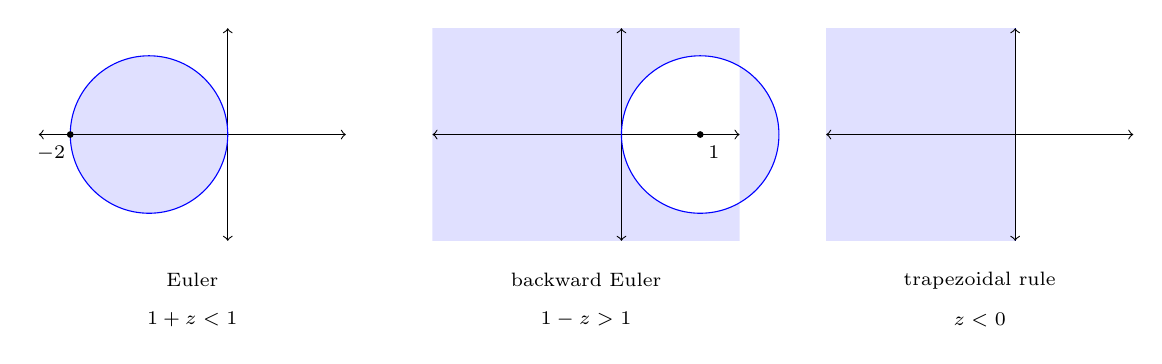
\begin{tikzpicture}
  % Euler
  \begin{scope}
    \fill[blue!12] (-1,0) circle (1);
    \draw[<->,thin] (-2.4,0) -- (1.5,0);
    \draw[<->,thin] (0,-1.35) -- (0,1.35);
    \draw[thin,color=blue] (-1,0) circle (1);
    \filldraw[black] (-2,0) circle (1.0pt);
    \node[below left] at (-1.94,-0.02) {\scriptsize $-2$};
    \node at (-0.45,-1.85) {\scriptsize Euler};
    \node at (-0.45,-2.35) {\scriptsize $\abs{1+z} < 1$};
  \end{scope}
  % Backward Euler
  \begin{scope}[xshift=5.0cm]
    \fill[blue!12,even odd rule] (-2.4,-1.35) rectangle (1.5,1.35) (1,0) circle (1);
    \draw[<->,thin] (-2.4,0) -- (1.5,0);
    \draw[<->,thin] (0,-1.35) -- (0,1.35);
    \draw[thin,color=blue] (1,0) circle (1);
    \filldraw[black] (1,0) circle (1.0pt);
    \node[below right] at (0.98,-0.02) {\scriptsize $1$};
    \node at (-0.45,-1.85) {\scriptsize backward Euler};
    \node at (-0.45,-2.35) {\scriptsize $\abs{1-z} > 1$};
  \end{scope}
  % Trapezoidal
  \begin{scope}[xshift=10.0cm]
    \fill[blue!12] (-2.4,-1.35) rectangle (0,1.35);
    \draw[<->,thin] (-2.4,0) -- (1.5,0);
    \draw[thin,color=blue] (0,-1.35) -- (0,1.35);
    \draw[<->,thin] (0,-1.35) -- (0,1.35);
    \node at (-0.45,-1.85) {\scriptsize trapezoidal rule};
    \node at (-0.45,-2.35) {\scriptsize $\re z < 0$};
  \end{scope}
\end{tikzpicture}
\end{center}

The contrast is striking. The explicit method has a bounded stability domain, so for any fixed $\lambda$ with $\re\lambda \ll 0$ there is a hard ceiling on $h$; the two implicit methods have no such ceiling at all. This is the pay-off that justifies the extra work of solving an implicit equation at each step, and it is why stiff problems are solved with implicit methods.

\begin{remark}
  The trapezoidal rule is A-stable but its $r(z)$ satisfies $\abs{r(z)} \to 1$ as $\abs{z}\to\infty$, so very stiff components are barely damped -- they merely oscillate in sign. Backward Euler has $r(z) \to 0$, and kills them outright. A method with $r(\infty) = 0$ is called \emph{L-stable}, and for genuinely stiff problems this is what one wants.
\end{remark}

\subsection{Stability of Multistep and Runge--Kutta Methods}

For a multistep method the analysis is a little different, since the recurrence is of order $s$. Applying the method to $y' = \lambda y$ with $z = h\lambda$ gives
$$
\sum_{\ell=0}^{s}\rho_\ell y_{n+\ell} = z\sum_{\ell=0}^s \sigma_\ell y_{n+\ell}, \qquad \text{i.e.}\qquad \sum_{\ell=0}^s (\rho_\ell - z\sigma_\ell)y_{n+\ell} = 0.
$$
This is a linear recurrence with characteristic polynomial $\rho(w) - z\sigma(w)$, and its solutions tend to zero exactly when all the roots of that polynomial lie strictly inside the unit disc. So
$$
\mathcal{D} = \{z \in \C : \text{all roots } w \text{ of } \rho(w) - z\sigma(w) \text{ satisfy } \abs{w} < 1\}.
$$
Notice that $z = 0$ gives back the root condition (in its non-strict form), which is reassuring: linear stability at $z = 0$ is exactly convergence.

This is harder to work with, and the news is bad.

\begin{theorem}[Second Dahlquist Barrier]
  No A-stable multistep method has order greater than $2$. Among the A-stable multistep methods of order $2$, the trapezoidal rule has the smallest error constant.
\end{theorem}

We do not prove this. It is a genuine obstruction rather than a failure of ingenuity, and it forces a choice: either accept low order, or weaken the demand for A-stability, or leave the multistep world altogether.

The second option is what is done in practice. Many stiff systems have eigenvalues that are not merely in $\C^-$ but far from the imaginary axis, so it suffices to have a stability domain containing a wedge around the negative real axis. A method whose stability domain contains such a wedge $\{z : \abs{\arg(-z)} < \alpha\}$ is called \emph{$A(\alpha)$-stable}, and the BDF methods of order up to $6$ all have this property with a decent $\alpha$. This is why they exist.

The third option is Runge--Kutta. Applying a Runge--Kutta method to $y' = \lambda y$ always gives $y_{n+1} = r(z)y_n$ for a rational function $r$, so $\mathcal{D} = \{z : \abs{r(z)} < 1\}$; and there is no barrier theorem here.

\begin{example}[An A-stable Implicit Runge--Kutta Method]
  Consider the two-stage implicit method with tableau
  $$
  \begin{array}{c|cc}
    0 & \tfrac14 & -\tfrac14\\[2pt]
    \tfrac23 & \tfrac14 & \tfrac{5}{12}\\[2pt]\hline
      & \tfrac14 & \tfrac34
  \end{array},
  $$
  that is,
  $$
  k_1 = f\left(t_n, y_n + \tfrac{h}{4}(k_1 - k_2)\right), \quad k_2 = f\left(t_n + \tfrac{2h}{3}, y_n + \tfrac{h}{12}(3k_1 + 5k_2)\right),
  $$
  with $y_{n+1} = y_n + \tfrac{h}{4}(k_1 + 3k_2)$. Applying this to $y' = \lambda y$ and eliminating $k_1, k_2$ gives $y_{n+1} = r(z)y_n$ with
  $$
  r(z) = \frac{6 + 2z}{6 - 4z + z^2}.
  $$
  We claim $\mathcal{D} \supseteq \C^-$. The denominator $z^2 - 4z + 6$ has roots $2 \pm i\sqrt 2$, both in the right half-plane, so $r$ is analytic on $\overline{\C^-}$; and $r(z) \to 0$ as $\abs z \to \infty$. By the maximum modulus principle, $\abs{r}$ attains its maximum over the closed left half-plane on the boundary, so it suffices to check $\abs{r(ix)} \leq 1$ for $x \in \R$. Now
  $$
  \abs{6 + 2ix}^2 = 36 + 4x^2, \qquad \abs{6 - x^2 - 4ix}^2 = (6-x^2)^2 + 16x^2 = 36 + 4x^2 + x^4,
  $$
  so $\abs{r(ix)}^2 = \frac{36+4x^2}{36+4x^2+x^4} \leq 1$, with equality only at $x = 0$. Hence $\abs{r(z)} < 1$ throughout $\C^-$, and the method is A-stable. It can be shown that it also has order $3$ -- beating the Dahlquist barrier comfortably.
\end{example}

\begin{remark}
  The same argument shows the $\nu$-stage Gauss--Legendre methods are all A-stable; the two-stage one has
  $$
  r(z) = \frac{12 + 6z + z^2}{12 - 6z + z^2},
  $$
  for which $\abs{r(ix)} = 1$ for all real $x$, so its stability domain is exactly $\C^-$. Order $4$ and exact stability, in two stages -- at the price of solving a coupled implicit system at every step.
\end{remark}

\subsection{Implementation}

We close the discussion of differential equations with a few words on what one actually does, since the theory above leaves two practical questions unanswered: how big should $h$ be, and how do we solve the implicit equations?

\subsubsection*{Choosing the step size}

A user of an ODE solver does not want to specify $h$; they want to specify an error tolerance $\varepsilon$ and have the solver work out $h$ for itself, varying it as the solution demands. To do that we need a cheap estimate of the local error at each step.

\begin{method}[The Milne Device]
  Run two multistep methods of the same order side by side, one explicit (the \emph{predictor}) and one implicit (the \emph{corrector}). If the two methods have error constants $c_P$ and $c_C$, then
  $$
  y^{P}_{n+1} \approx y(t_{n+1}) - c_P h^{p+1}y^{(p+1)}(t_n), \qquad y^{C}_{n+1} \approx y(t_{n+1}) - c_C h^{p+1}y^{(p+1)}(t_n).
  $$
  Subtracting eliminates the unknown derivative,
  $$
  h^{p+1}y^{(p+1)}(t_n) \approx \frac{y^P_{n+1} - y^C_{n+1}}{c_C - c_P},
  $$
  and substituting back gives the estimate
  $$
  y^C_{n+1} - y(t_{n+1}) \approx \frac{c_C}{c_C - c_P}\left(y^P_{n+1} - y^C_{n+1}\right)
  $$
  for the local error of the corrector, computable from quantities we have already.
\end{method}

\begin{example}
  With the two-step Adams--Bashforth method as predictor ($c_P = \tfrac{5}{12}$) and the trapezoidal rule as corrector ($c_C = -\tfrac1{12}$), the estimate is
  $$
  y^{C}_{n+1} - y(t_{n+1}) \approx -\tfrac16\left(y^{P}_{n+1} - y^{C}_{n+1}\right).
  $$
  The predictor costs one extra evaluation of $f$, which is cheap, and it doubles as an excellent starting guess for the implicit corrector equation.
\end{example}

Given the estimate, the logic is straightforward: if it exceeds the tolerance $\varepsilon$, reject the step and retry with smaller $h$; if it is comfortably below (say below $\varepsilon/10$), accept the step and increase $h$; otherwise accept and carry on unchanged.

For Runge--Kutta methods there is no single error constant to exploit, and the analogous device is \emph{embedded} Runge--Kutta: one uses two methods, of orders $p$ and $p+1$, sharing as many stages as possible so that the extra accuracy is nearly free.

\begin{example}[An Embedded Pair]
  With
  $$
  k_1 = f(t_n,y_n), \quad k_2 = f\left(t_n + \tfrac{h}{2}, y_n + \tfrac{h}{2}k_1\right), \quad k_3 = f\left(t_n + h, y_n - hk_1 + 2hk_2\right),
  $$
  the combination $y^{[1]}_{n+1} = y_n + hk_2$ has order $2$, while $y^{[2]}_{n+1} = y_n + \tfrac{h}{6}(k_1 + 4k_2 + k_3)$ has order $3$. The difference $y^{[1]}_{n+1} - y^{[2]}_{n+1}$ estimates the error in the lower-order formula, at the cost of three function evaluations in total.
\end{example}

\subsubsection*{Solving the implicit equations}

An implicit method requires us to solve, at each step, an equation of the form
$$
y_{n+s} = h\sigma_s f(t_{n+s}, y_{n+s}) + v,
$$
where $v$ collects everything already known. The simplest approach is \vocab{functional iteration},
$$
y^{[j+1]}_{n+s} = h\sigma_s f\left(t_{n+s}, y^{[j]}_{n+s}\right) + v,
$$
started from the predictor. This is a contraction provided $h\abs{\sigma_s}\lambda < 1$, where $\lambda$ is the Lipschitz constant of $f$ -- but that is precisely the sort of restriction on $h$ we adopted an implicit method to escape. So for stiff problems functional iteration is useless, and one uses the \vocab{Newton--Raphson} method instead: setting $\psi(y) = y - h\sigma_s f(t_{n+s},y) - v$, iterate
$$
y^{[j+1]}_{n+s} = y^{[j]}_{n+s} - \left(D\psi\left(y^{[j]}_{n+s}\right)\right)^{-1}\psi\left(y^{[j]}_{n+s}\right),
$$
which converges quadratically from a good starting guess. Evaluating and inverting the Jacobian $D\psi = I - h\sigma_s D_yf$ at every iteration is expensive, so in practice one freezes it,
$$
y^{[j+1]}_{n+s} = y^{[j]}_{n+s} - \left(D\psi\left(y^{[0]}_{n+s}\right)\right)^{-1}\psi\left(y^{[j]}_{n+s}\right),
$$
recomputing only when convergence deteriorates. Either way we are left with a linear system to solve at every step, usually with the same matrix many times over -- which is exactly the situation the next section is designed for.


\section{Numerical Linear Algebra}

Solving $A\mathbf{x} = \mathbf{b}$ is the single most common task in scientific computing, and one that we have already run into twice in this course -- in the normal equations for least-squares fitting, and in the Newton iteration for implicit ODE methods. In pure linear algebra the problem is considered solved: $\mathbf{x} = A^{-1}\mathbf{b}$, and Cramer's rule even gives a formula. But Cramer's rule for a $20\times 20$ system requires more arithmetic than has been performed in the history of the world, so we shall have to do better.

The strategy throughout is \emph{factorisation}: write $A$ as a product of matrices for which the system is easy, solve a sequence of easy systems, and -- crucially -- reuse the factorisation if the same $A$ appears again with a different $\mathbf{b}$.

\subsection{Triangular Systems}

The easy case is a triangular matrix.

\begin{definition}
  A square matrix $L$ is \vocab{lower triangular} if $L_{ij} = 0$ for $j > i$, and \vocab{unit} lower triangular if in addition $L_{ii} = 1$ for all $i$. Similarly $U$ is \vocab{upper triangular} if $U_{ij} = 0$ for $j < i$.
\end{definition}

If $L$ is lower triangular and nonsingular, the system $L\mathbf{y} = \mathbf{b}$ is solved by \emph{forward substitution}: the first equation gives $y_1 = b_1/L_{11}$, and having found $y_1, \dots, y_{i-1}$ the $i$-th equation gives
$$
y_i = \frac{1}{L_{ii}}\left(b_i - \sum_{j<i}L_{ij}y_j\right).
$$
This costs $\mathcal{O}(n^2)$ operations, one multiplication for each nonzero entry of $L$. Upper triangular systems are solved the same way from the bottom up, by \emph{back substitution}.

\subsection{LU Factorisation}

\begin{definition}[LU Factorisation]
  An \vocab{LU factorisation} of a square matrix $A$ is a factorisation $A = LU$ in which $L$ is unit lower triangular and $U$ is upper triangular.
\end{definition}

Given such a factorisation, everything becomes cheap. To solve $A\mathbf{x} = \mathbf{b}$ we solve $L\mathbf{y} = \mathbf{b}$ by forward substitution and then $U\mathbf{x} = \mathbf{y}$ by back substitution, at a cost of $\mathcal{O}(n^2)$ for each new right-hand side. The determinant is
$$
\det A = \det L \det U = \prod_{i=1}^n U_{ii},
$$
so $A$ is singular precisely when some $U_{ii} = 0$.

How do we compute it? Write $\mathbf{l}_1, \dots, \mathbf{l}_n$ for the columns of $L$ and $\mathbf{u}_1^\top, \dots, \mathbf{u}_n^\top$ for the rows of $U$. Then
$$
A = LU = \sum_{k=1}^{n}\mathbf{l}_k \mathbf{u}_k^\top,
$$
an expression of $A$ as a sum of $n$ rank-one matrices. The point is that $\mathbf{l}_k$ has zeros in its first $k-1$ entries and $\mathbf{u}_k$ has zeros in its first $k-1$ entries, so $\mathbf{l}_k\mathbf{u}_k^\top$ has zeros in its first $k-1$ rows \emph{and} its first $k-1$ columns. Consequently the first row and column of $A$ come entirely from the $k=1$ term, and we can read them off.

\begin{method}[LU by Outer Products]
  Set $A_0 = A$. For $k = 1, 2, \dots, n$:
  \begin{enumerate}[label=(\roman*)]
    \item let $\mathbf{u}_k^\top$ be the $k$-th row of $A_{k-1}$;
    \item let $\mathbf{l}_k$ be the $k$-th column of $A_{k-1}$, divided by $(A_{k-1})_{kk}$ so that $(\mathbf{l}_k)_k = 1$;
    \item set $A_k = A_{k-1} - \mathbf{l}_k\mathbf{u}_k^\top$.
  \end{enumerate}
  Then $A = \sum_k \mathbf{l}_k\mathbf{u}_k^\top = LU$.
\end{method}

At step $k$ the dominant cost is forming the outer product, which touches an $(n-k+1)\times(n-k+1)$ block, so the total cost is $\sum_k (n-k+1)^2 \sim \tfrac13 n^3$ operations. This is the same $\mathcal{O}(n^3)$ as Gaussian elimination -- indeed, the algorithm \emph{is} Gaussian elimination, with the multipliers recorded in $L$ instead of discarded. The advantage of keeping them is that a second right-hand side then costs only $\mathcal{O}(n^2)$ rather than another $\mathcal{O}(n^3)$.

\begin{example}
  Let
  $$
  A = \begin{pmatrix} 2 & 1 & 1\\ 4 & 3 & 3\\ 8 & 7 & 9\end{pmatrix}.
  $$
  Step $1$: $\mathbf{u}_1^\top = (2,1,1)$ and $\mathbf{l}_1 = (1,2,4)^\top$, so
  $$
  A_1 = A - \begin{pmatrix}1\\2\\4\end{pmatrix}(2,1,1) = \begin{pmatrix}0&0&0\\0&1&1\\0&3&5\end{pmatrix}.
  $$
  Step $2$: $\mathbf{u}_2^\top = (0,1,1)$ and $\mathbf{l}_2 = (0,1,3)^\top$, giving
  $$
  A_2 = A_1 - \begin{pmatrix}0\\1\\3\end{pmatrix}(0,1,1) = \begin{pmatrix}0&0&0\\0&0&0\\0&0&2\end{pmatrix}.
  $$
  Step $3$: $\mathbf{u}_3^\top = (0,0,2)$, $\mathbf{l}_3 = (0,0,1)^\top$. Hence
  $$
  L = \begin{pmatrix}1&0&0\\2&1&0\\4&3&1\end{pmatrix}, \qquad U = \begin{pmatrix}2&1&1\\0&1&1\\0&0&2\end{pmatrix},
  $$
  and $\det A = 2 \cdot 1\cdot 2 = 4$.
\end{example}

The algorithm breaks down if $(A_{k-1})_{kk} = 0$, since we cannot divide by it. Sometimes this is unavoidable: the matrix $\begin{psmallmatrix}0&1\\1&0\end{psmallmatrix}$ has no LU factorisation at all, as one sees immediately by multiplying out $\begin{psmallmatrix}1&0\\ \ell&1\end{psmallmatrix}\begin{psmallmatrix}u_{11}&u_{12}\\0&u_{22}\end{psmallmatrix}$ and comparing top-left entries. The precise condition is the following.

\begin{theorem}[Existence and Uniqueness of LU]\label{thm:luexist}
  Let $A$ be $n\times n$ and let $A^{(k)}$ denote its leading $k\times k$ principal submatrix. If $A^{(k)}$ is nonsingular for every $k = 1, \dots, n$, then $A$ has an LU factorisation, and it is unique.
\end{theorem}
\begin{proof}
  \emph{Uniqueness} first, and note that it does not need the hypothesis beyond $A$ being nonsingular. Suppose $A = LU = L'U'$ with $L, L'$ unit lower triangular and $U, U'$ upper triangular and nonsingular. Then $(L')^{-1}L = U'U^{-1}$. The left side is unit lower triangular (inverses and products of unit lower triangular matrices are unit lower triangular) and the right side is upper triangular. A matrix that is both is diagonal, and being unit lower triangular it must be $I$. Hence $L = L'$ and $U = U'$.

  \emph{Existence}, by induction on $k$, constructing the factorisation of $A^{(k)}$. For $k = 1$, take $L = (1)$ and $U = (A_{11})$, which is legitimate since $A^{(1)} \neq 0$. Suppose $A^{(k)} = L_kU_k$ with $L_k$ unit lower triangular and $U_k$ upper triangular; since $\det A^{(k)} = \det U_k \neq 0$, both factors are nonsingular. Write
  $$
  A^{(k+1)} = \begin{pmatrix} A^{(k)} & \mathbf{b}\\ \mathbf{c}^\top & d\end{pmatrix},
  $$
  and look for a factorisation
  $$
  A^{(k+1)} = \begin{pmatrix}L_k & \mathbf{0}\\ \mathbf{x}^\top & 1\end{pmatrix}\begin{pmatrix}U_k & \mathbf{y}\\ \mathbf{0}^\top & u\end{pmatrix} = \begin{pmatrix}L_kU_k & L_k\mathbf{y}\\ \mathbf{x}^\top U_k & \mathbf{x}^\top\mathbf{y} + u\end{pmatrix}.
  $$
  The top-left block is already correct. The remaining equations are $L_k\mathbf{y} = \mathbf{b}$, $U_k^\top \mathbf{x} = \mathbf{c}$ and $u = d - \mathbf{x}^\top\mathbf{y}$, and each has a unique solution because $L_k$ and $U_k$ are nonsingular. This completes the induction, and taking $k = n$ gives the result.
\end{proof}

\begin{remark}
  The hypothesis is sufficient but not necessary: the zero matrix has an LU factorisation (many of them) while all its principal minors vanish. What the theorem really says is that if the leading minors are nonsingular, the naive algorithm never has to divide by zero -- and the pivots it uses are exactly $U_{kk} = \det A^{(k)}/\det A^{(k-1)}$.
\end{remark}

\subsection{Pivoting}

A zero pivot is fatal, and -- worse -- a \emph{small} pivot is nearly fatal, since dividing by it amplifies whatever rounding error is present. The cure for both is to reorder the rows.

\begin{method}[LU with Partial Pivoting]
  At step $k$, before doing anything else, choose $p \geq k$ maximising $\abs{(A_{k-1})_{pk}}$ and let $P_k$ be the permutation matrix exchanging rows $k$ and $p$. Then take $\mathbf{u}_k^\top$ to be the $k$-th row of $P_kA_{k-1}$, take
  $$
  \mathbf{l}_k = \frac{1}{(P_kA_{k-1})_{kk}}\left(k\text{-th column of }P_kA_{k-1}\right),
  $$
  and set $A_k = P_kA_{k-1} - \mathbf{l}_k\mathbf{u}_k^\top$.
\end{method}

Choosing the largest available entry guarantees that every entry of $\mathbf{l}_k$ has modulus at most $1$, so the multipliers never magnify errors. Unwinding the algorithm, one finds
$$
(P_{n-1}\cdots P_1)A = \tilde{\mathbf{l}}_1\mathbf{u}_1^\top + \cdots + \tilde{\mathbf{l}}_n\mathbf{u}_n^\top, \qquad \tilde{\mathbf{l}}_k = P_{n-1}\cdots P_{k+1}\mathbf{l}_k,
$$
and since the permutations applied to $\mathbf{l}_k$ only touch entries from position $k+1$ onwards, the vectors $\tilde{\mathbf{l}}_k$ still have zeros in their first $k-1$ places. So they are the columns of a unit lower triangular matrix, and we have proved the following.

\begin{theorem}[LU with Pivoting]
  For any square matrix $A$ there is a permutation matrix $P$ such that $PA = LU$ with $L$ unit lower triangular and $U$ upper triangular.
\end{theorem}
\begin{proof}
  Run the algorithm above, taking $P = P_{n-1}\cdots P_1$. The only remaining worry is a step at which the entire $k$-th column of $A_{k-1}$ (from row $k$ down) is zero; in that case there is nothing to eliminate, and we may simply take $P_k = I$, $\mathbf{l}_k = \mathbf{e}_k$ and $\mathbf{u}_k^\top$ the $k$-th row of $A_{k-1}$, which preserves everything we need.
\end{proof}

To solve $A\mathbf{x} = \mathbf{b}$ we then solve $L\mathbf{y} = P\mathbf{b}$ and $U\mathbf{x} = \mathbf{y}$; permuting a vector is free.

\subsection{Symmetric Matrices and Cholesky}

When $A$ is symmetric it is wasteful to compute both $L$ and $U$, since we ought to be able to get one from the other. The right factorisation is the following.

\begin{definition}
  An \vocab{$LDL^\top$ factorisation} of a symmetric matrix $A$ is a factorisation $A = LDL^\top$ with $L$ unit lower triangular and $D$ diagonal.
\end{definition}

Setting $U = DL^\top$ recovers an LU factorisation, so by Theorem \ref{thm:luexist} the $LDL^\top$ factorisation is unique when it exists. It is computed by exactly the same outer-product scheme: writing $A = \sum_k D_{kk}\mathbf{l}_k\mathbf{l}_k^\top$, we set $A_0 = A$, take $D_{kk} = (A_{k-1})_{kk}$, take $\mathbf{l}_k$ to be the $k$-th column of $A_{k-1}$ scaled so that $(\mathbf{l}_k)_k = 1$, and put $A_k = A_{k-1} - D_{kk}\mathbf{l}_k\mathbf{l}_k^\top$. Since we only need the lower half of each $A_k$, the work is halved.

\begin{example}
  Take $A = \begin{pmatrix}2&4\\4&11\end{pmatrix}$. Then $D_{11} = 2$ and $\mathbf{l}_1 = (1,2)^\top$, so
  $$
  A_1 = \begin{pmatrix}2&4\\4&11\end{pmatrix} - 2\begin{pmatrix}1\\2\end{pmatrix}(1,2) = \begin{pmatrix}0&0\\0&3\end{pmatrix},
  $$
  whence $D_{22} = 3$, $\mathbf{l}_2 = (0,1)^\top$ and
  $$
  A = \begin{pmatrix}1&0\\2&1\end{pmatrix}\begin{pmatrix}2&0\\0&3\end{pmatrix}\begin{pmatrix}1&2\\0&1\end{pmatrix}.
  $$
\end{example}

\begin{definition}
  A symmetric matrix $A$ is \vocab{positive definite} if $\mathbf{x}^\top A\mathbf{x} > 0$ for every $\mathbf{x}\neq \mathbf{0}$.
\end{definition}

\begin{theorem}\label{thm:posdef}
  A real symmetric matrix $A$ is positive definite if and only if it has an $LDL^\top$ factorisation in which every diagonal entry of $D$ is positive.
\end{theorem}
\begin{proof}
  ($\Leftarrow$) If $A = LDL^\top$ with $D_{kk} > 0$, then for $\mathbf{x}\neq\mathbf{0}$ put $\mathbf{z} = L^\top\mathbf{x}$, which is nonzero since $L^\top$ is nonsingular. Then $\mathbf{x}^\top A\mathbf{x} = \mathbf{z}^\top D\mathbf{z} = \sum_k D_{kk}z_k^2 > 0$.

  ($\Rightarrow$) Suppose $A$ is positive definite. Every leading principal submatrix $A^{(k)}$ is then positive definite (test with vectors supported on the first $k$ coordinates), hence nonsingular, so by Theorem \ref{thm:luexist} the factorisation exists. Its diagonal entries satisfy $D_{kk} = \det A^{(k)}/\det A^{(k-1)}$, and all these determinants are positive because a positive definite matrix has positive determinant (its eigenvalues are all positive). Hence $D_{kk} > 0$.
\end{proof}

\begin{definition}[Cholesky Factorisation]
  If $A$ is symmetric positive definite, write $D^{1/2}$ for the diagonal matrix with entries $\sqrt{D_{kk}}$ and set $\tilde L = LD^{1/2}$. Then
  $$
  A = \tilde L\tilde L^\top
  $$
  with $\tilde L$ lower triangular with positive diagonal. This is the \vocab{Cholesky factorisation}.
\end{definition}

Cholesky is the workhorse for symmetric positive definite systems. It needs no pivoting -- the theorem guarantees the pivots are positive, and one can show they cannot grow -- it uses half the storage and half the arithmetic of LU, and it fails, in a numerically detectable way, precisely when $A$ is not positive definite. That last property makes it the standard test for positive definiteness.

\subsection{Banded and Sparse Matrices}

Large matrices arising in practice are rarely dense. Discretising a differential equation, for instance, couples each unknown only to its neighbours, and the resulting matrix has almost all entries zero. It would be a shame to spend $\mathcal{O}(n^3)$ operations on such a matrix, and we need not.

\begin{theorem}[Inheritance of Zeros]\label{thm:inherit}
  Let $A = LU$ be an LU factorisation. If $A_{ij} = 0$ for all $j \le m$ (that is, row $i$ of $A$ begins with $m$ zeros, with $m < i$), then $L_{ij} = 0$ for $j \le m$; and symmetrically, leading zeros in the columns of $A$ above the diagonal are inherited by $U$.
\end{theorem}
\begin{proof}
  We induct on $j$. Suppose $A_{i1} = 0$. Since $A_{i1} = \sum_k L_{ik}U_{k1} = L_{i1}U_{11}$ and $U_{11}\neq 0$, we get $L_{i1} = 0$. Now suppose $L_{i1} = \cdots = L_{i,j-1} = 0$ and $A_{ij} = 0$ with $j < i$. Then
  $$
  0 = A_{ij} = \sum_{k\leq j}L_{ik}U_{kj} = L_{ij}U_{jj},
  $$
  and $U_{jj}\neq 0$ gives $L_{ij} = 0$. The statement for $U$ follows by applying this to $A^\top$.
\end{proof}

\begin{definition}[Banded Matrix]
  A matrix $A$ is \vocab{banded} with bandwidth $r$ if $A_{ij} = 0$ whenever $\abs{i-j} > r$.
\end{definition}

Combining the two: if $A$ is banded with bandwidth $r$, then row $i$ of $A$ begins with $i - r - 1$ zeros and so does row $i$ of $L$; likewise for $U$. So $L$ and $U$ are banded with the same bandwidth $r$, and the factorisation can be computed by touching only the band. The cost drops from $\mathcal{O}(n^3)$ to $\mathcal{O}(r^2 n)$, which for a tridiagonal matrix ($r=1$) is $\mathcal{O}(n)$.

The picture is worth a glance: shaded cells are the ones that may be nonzero.
\begin{center}
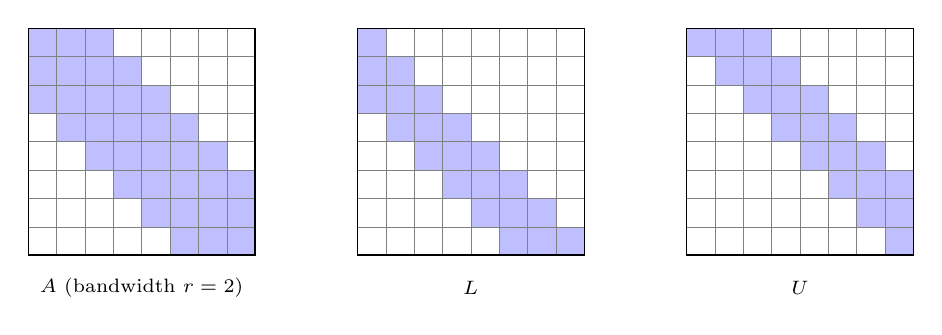
\begin{tikzpicture}
  \begin{scope}[xshift=0.00cm]
    \fill[blue!25] (0.000,-0.360) rectangle (0.360,0.000);
    \fill[blue!25] (0.360,-0.360) rectangle (0.720,0.000);
    \fill[blue!25] (0.720,-0.360) rectangle (1.080,0.000);
    \fill[blue!25] (0.000,-0.720) rectangle (0.360,-0.360);
    \fill[blue!25] (0.360,-0.720) rectangle (0.720,-0.360);
    \fill[blue!25] (0.720,-0.720) rectangle (1.080,-0.360);
    \fill[blue!25] (1.080,-0.720) rectangle (1.440,-0.360);
    \fill[blue!25] (0.000,-1.080) rectangle (0.360,-0.720);
    \fill[blue!25] (0.360,-1.080) rectangle (0.720,-0.720);
    \fill[blue!25] (0.720,-1.080) rectangle (1.080,-0.720);
    \fill[blue!25] (1.080,-1.080) rectangle (1.440,-0.720);
    \fill[blue!25] (1.440,-1.080) rectangle (1.800,-0.720);
    \fill[blue!25] (0.360,-1.440) rectangle (0.720,-1.080);
    \fill[blue!25] (0.720,-1.440) rectangle (1.080,-1.080);
    \fill[blue!25] (1.080,-1.440) rectangle (1.440,-1.080);
    \fill[blue!25] (1.440,-1.440) rectangle (1.800,-1.080);
    \fill[blue!25] (1.800,-1.440) rectangle (2.160,-1.080);
    \fill[blue!25] (0.720,-1.800) rectangle (1.080,-1.440);
    \fill[blue!25] (1.080,-1.800) rectangle (1.440,-1.440);
    \fill[blue!25] (1.440,-1.800) rectangle (1.800,-1.440);
    \fill[blue!25] (1.800,-1.800) rectangle (2.160,-1.440);
    \fill[blue!25] (2.160,-1.800) rectangle (2.520,-1.440);
    \fill[blue!25] (1.080,-2.160) rectangle (1.440,-1.800);
    \fill[blue!25] (1.440,-2.160) rectangle (1.800,-1.800);
    \fill[blue!25] (1.800,-2.160) rectangle (2.160,-1.800);
    \fill[blue!25] (2.160,-2.160) rectangle (2.520,-1.800);
    \fill[blue!25] (2.520,-2.160) rectangle (2.880,-1.800);
    \fill[blue!25] (1.440,-2.520) rectangle (1.800,-2.160);
    \fill[blue!25] (1.800,-2.520) rectangle (2.160,-2.160);
    \fill[blue!25] (2.160,-2.520) rectangle (2.520,-2.160);
    \fill[blue!25] (2.520,-2.520) rectangle (2.880,-2.160);
    \fill[blue!25] (1.800,-2.880) rectangle (2.160,-2.520);
    \fill[blue!25] (2.160,-2.880) rectangle (2.520,-2.520);
    \fill[blue!25] (2.520,-2.880) rectangle (2.880,-2.520);
    \draw[ultra thin,color=gray] (0,0) grid[xstep=0.360,ystep=0.360] (2.880,-2.880);
    \draw[thin] (0,0) rectangle (2.880,-2.880);
    \node at (1.440,-3.300) {\scriptsize $A$ (bandwidth $r=2$)};
  \end{scope}
  \begin{scope}[xshift=4.18cm]
    \fill[blue!25] (0.000,-0.360) rectangle (0.360,0.000);
    \fill[blue!25] (0.000,-0.720) rectangle (0.360,-0.360);
    \fill[blue!25] (0.360,-0.720) rectangle (0.720,-0.360);
    \fill[blue!25] (0.000,-1.080) rectangle (0.360,-0.720);
    \fill[blue!25] (0.360,-1.080) rectangle (0.720,-0.720);
    \fill[blue!25] (0.720,-1.080) rectangle (1.080,-0.720);
    \fill[blue!25] (0.360,-1.440) rectangle (0.720,-1.080);
    \fill[blue!25] (0.720,-1.440) rectangle (1.080,-1.080);
    \fill[blue!25] (1.080,-1.440) rectangle (1.440,-1.080);
    \fill[blue!25] (0.720,-1.800) rectangle (1.080,-1.440);
    \fill[blue!25] (1.080,-1.800) rectangle (1.440,-1.440);
    \fill[blue!25] (1.440,-1.800) rectangle (1.800,-1.440);
    \fill[blue!25] (1.080,-2.160) rectangle (1.440,-1.800);
    \fill[blue!25] (1.440,-2.160) rectangle (1.800,-1.800);
    \fill[blue!25] (1.800,-2.160) rectangle (2.160,-1.800);
    \fill[blue!25] (1.440,-2.520) rectangle (1.800,-2.160);
    \fill[blue!25] (1.800,-2.520) rectangle (2.160,-2.160);
    \fill[blue!25] (2.160,-2.520) rectangle (2.520,-2.160);
    \fill[blue!25] (1.800,-2.880) rectangle (2.160,-2.520);
    \fill[blue!25] (2.160,-2.880) rectangle (2.520,-2.520);
    \fill[blue!25] (2.520,-2.880) rectangle (2.880,-2.520);
    \draw[ultra thin,color=gray] (0,0) grid[xstep=0.360,ystep=0.360] (2.880,-2.880);
    \draw[thin] (0,0) rectangle (2.880,-2.880);
    \node at (1.440,-3.300) {\scriptsize $L$};
  \end{scope}
  \begin{scope}[xshift=8.36cm]
    \fill[blue!25] (0.000,-0.360) rectangle (0.360,0.000);
    \fill[blue!25] (0.360,-0.360) rectangle (0.720,0.000);
    \fill[blue!25] (0.720,-0.360) rectangle (1.080,0.000);
    \fill[blue!25] (0.360,-0.720) rectangle (0.720,-0.360);
    \fill[blue!25] (0.720,-0.720) rectangle (1.080,-0.360);
    \fill[blue!25] (1.080,-0.720) rectangle (1.440,-0.360);
    \fill[blue!25] (0.720,-1.080) rectangle (1.080,-0.720);
    \fill[blue!25] (1.080,-1.080) rectangle (1.440,-0.720);
    \fill[blue!25] (1.440,-1.080) rectangle (1.800,-0.720);
    \fill[blue!25] (1.080,-1.440) rectangle (1.440,-1.080);
    \fill[blue!25] (1.440,-1.440) rectangle (1.800,-1.080);
    \fill[blue!25] (1.800,-1.440) rectangle (2.160,-1.080);
    \fill[blue!25] (1.440,-1.800) rectangle (1.800,-1.440);
    \fill[blue!25] (1.800,-1.800) rectangle (2.160,-1.440);
    \fill[blue!25] (2.160,-1.800) rectangle (2.520,-1.440);
    \fill[blue!25] (1.800,-2.160) rectangle (2.160,-1.800);
    \fill[blue!25] (2.160,-2.160) rectangle (2.520,-1.800);
    \fill[blue!25] (2.520,-2.160) rectangle (2.880,-1.800);
    \fill[blue!25] (2.160,-2.520) rectangle (2.520,-2.160);
    \fill[blue!25] (2.520,-2.520) rectangle (2.880,-2.160);
    \fill[blue!25] (2.520,-2.880) rectangle (2.880,-2.520);
    \draw[ultra thin,color=gray] (0,0) grid[xstep=0.360,ystep=0.360] (2.880,-2.880);
    \draw[thin] (0,0) rectangle (2.880,-2.880);
    \node at (1.440,-3.300) {\scriptsize $U$};
  \end{scope}
\end{tikzpicture}
\end{center}

\begin{remark}
  For a general sparse matrix -- one with many zeros but no particular pattern -- the situation is more delicate, because elimination can create nonzeros where there were none. This is called \emph{fill-in}, and minimising it by reordering rows and columns is a genuinely hard combinatorial problem, attacked in practice with graph-theoretic heuristics. Iterative methods, which never form a factorisation at all, are the other standard response. Both are beyond this course, and both are covered in Part II.
\end{remark}


\section{QR Factorisation and Least Squares}\label{sec:qr}

The LU factorisation is fast, but it is not always well behaved: the factors can be much larger than $A$ itself, and errors can grow accordingly. Orthogonal matrices, by contrast, preserve lengths exactly, and so cannot amplify anything. This makes them the tool of choice when accuracy matters more than speed -- and, as we shall see, they are exactly what is needed for the least-squares problem.

\begin{definition}
  A set of vectors $\{\mathbf{q}_i\}$ in $\R^m$ is \vocab{orthonormal} if $\mathbf{q}_i^\top\mathbf{q}_j = \delta_{ij}$. A square matrix $Q$ is \vocab{orthogonal} if its columns are orthonormal, equivalently $Q^\top Q = I$, equivalently $Q^{-1} = Q^\top$.
\end{definition}

The key property is that orthogonal matrices are isometries: $\norm{Q\mathbf{x}}^2 = \mathbf{x}^\top Q^\top Q\mathbf{x} = \norm{\mathbf{x}}^2$. In particular $\abs{\det Q} = 1$, and multiplying by $Q$ can neither magnify nor shrink an error.

\begin{definition}[QR Factorisation]
  Let $A$ be $m\times n$. A \vocab{QR factorisation} of $A$ is a factorisation $A = QR$ with $Q$ an $m\times m$ orthogonal matrix and $R$ an $m\times n$ upper triangular matrix. If $m \geq n$, a \vocab{reduced} (or skinny) QR factorisation is $A = QR$ with $Q$ an $m\times n$ matrix with orthonormal columns and $R$ an $n\times n$ upper triangular matrix.
\end{definition}

If $A$ is square and nonsingular and $A = QR$, then $A\mathbf{x} = \mathbf{b}$ becomes $R\mathbf{x} = Q^\top\mathbf{b}$, a triangular system. So QR does everything LU does; it just costs about twice as much.

To see what a reduced QR factorisation \emph{means}, write $\mathbf{a}_1, \dots, \mathbf{a}_n$ for the columns of $A$ and $\mathbf{q}_1, \dots, \mathbf{q}_n$ for those of $Q$. Comparing columns in $A = QR$ and using upper-triangularity,
$$
\mathbf{a}_k = \sum_{j=1}^{k}R_{jk}\mathbf{q}_j .
$$
So $\mathbf{q}_1, \dots, \mathbf{q}_k$ is an orthonormal basis for the span of $\mathbf{a}_1, \dots, \mathbf{a}_k$, for every $k$. A reduced QR factorisation is nothing other than an orthonormalisation of the columns of $A$, carried out one column at a time. That immediately suggests an algorithm.

\subsection{Gram--Schmidt}

\begin{method}[Gram--Schmidt]
  Assume $m \geq n$ and that the columns of $A$ are linearly independent. Set
  $$
  R_{11} = \norm{\mathbf{a}_1}, \qquad \mathbf{q}_1 = \mathbf{a}_1/R_{11},
  $$
  and having found $\mathbf{q}_1, \dots, \mathbf{q}_{j-1}$, set
  $$
  R_{ij} = \mathbf{q}_i^\top\mathbf{a}_j \ (i < j), \qquad \mathbf{b}_j = \mathbf{a}_j - \sum_{i=1}^{j-1}R_{ij}\mathbf{q}_i, \qquad R_{jj} = \norm{\mathbf{b}_j}, \qquad \mathbf{q}_j = \mathbf{b}_j/R_{jj}.
  $$
\end{method}

The vector $\mathbf{b}_j$ is $\mathbf{a}_j$ with its components along $\mathbf{q}_1, \dots, \mathbf{q}_{j-1}$ removed, so it is orthogonal to all of them; and it is nonzero because the columns of $A$ are independent. The cost is $\mathcal{O}(mn^2)$.

This is the algorithm one meets in a first linear algebra course, and it is perfectly correct. Numerically, however, it is disappointing: the computed $\mathbf{q}_j$ drift out of orthogonality, because each is built from all its predecessors and their small errors compound. (Rearranging the arithmetic gives the `modified' Gram--Schmidt process, which is noticeably better, but still not ideal.) The trouble is philosophical as much as practical -- we are building an orthogonal matrix by a procedure that is not itself orthogonal.

The alternative is \emph{orthogonal triangularisation}: rather than orthogonalising the columns of $A$, multiply $A$ on the left by a sequence of orthogonal matrices, chosen to introduce zeros, until what is left is upper triangular. If
$$
\Omega_k \cdots \Omega_1 A = R
$$
with each $\Omega_i$ orthogonal, then $A = QR$ with $Q = (\Omega_k\cdots\Omega_1)^\top$, which is orthogonal by construction. We need a supply of orthogonal matrices that create zeros, and there are two standard choices.

\subsection{Givens Rotations}

\begin{definition}[Givens Rotation]
  For $1 \leq p < q \leq m$ and $\theta \in (-\pi,\pi]$, the \vocab{Givens rotation} $\Omega^{[p,q]}(\theta)$ is the $m\times m$ matrix equal to the identity except that
  $$
  \Omega_{pp} = \Omega_{qq} = \cos\theta, \qquad \Omega_{pq} = \sin\theta, \qquad \Omega_{qp} = -\sin\theta.
  $$
\end{definition}

Geometrically this is a rotation of the plane spanned by $\mathbf{e}_p$ and $\mathbf{e}_q$, leaving everything else fixed; it is clearly orthogonal. For $m = 4$, say,
$$
\Omega^{[1,2]} = \begin{pmatrix}\cos\theta & \sin\theta & 0&0\\ -\sin\theta&\cos\theta&0&0\\0&0&1&0\\0&0&0&1\end{pmatrix}, \qquad
\Omega^{[2,4]} = \begin{pmatrix}1&0&0&0\\0&\cos\theta&0&\sin\theta\\0&0&1&0\\0&-\sin\theta&0&\cos\theta\end{pmatrix}.
$$

\begin{proposition}\label{prop:givens}
  Let $A$ be $m\times n$, let $1 \leq p < q \leq m$ and $1\leq j \leq n$. Then there is $\theta$ such that $(\Omega^{[p,q]}A)_{qj} = 0$. Moreover $\Omega^{[p,q]}A$ agrees with $A$ in every row except the $p$-th and $q$-th, and those two rows are linear combinations of the $p$-th and $q$-th rows of $A$.
\end{proposition}
\begin{proof}
  The second and third statements hold for every $\theta$, directly from the definition. For the first, if $A_{pj} = A_{qj} = 0$ then any $\theta$ works. Otherwise take
  $$
  \cos\theta = \frac{A_{pj}}{\sqrt{A_{pj}^2 + A_{qj}^2}}, \qquad \sin\theta = \frac{A_{qj}}{\sqrt{A_{pj}^2 + A_{qj}^2}},
  $$
  which is a legitimate choice since the two squares sum to $1$. Then
  $$
  (\Omega^{[p,q]}A)_{qj} = -\sin\theta\, A_{pj} + \cos\theta\, A_{qj} = \frac{-A_{qj}A_{pj} + A_{pj}A_{qj}}{\sqrt{A_{pj}^2+A_{qj}^2}} = 0. \qedhere
  $$
\end{proof}

To triangularise $A$ we apply rotations that zero the subdiagonal entries one at a time, in an order that does not destroy the zeros already made. Because $\Omega^{[p,q]}$ only alters rows $p$ and $q$, taking the pairs $[p,q]$ in lexicographic order works: we clear column $1$ using $\Omega^{[1,2]}, \Omega^{[1,3]}, \dots, \Omega^{[1,m]}$, then column $2$ using $\Omega^{[2,3]}, \dots$, and so on.

\begin{example}
  For a $3\times 3$ matrix, $\Omega^{[2,3]}\Omega^{[1,3]}\Omega^{[1,2]}A$ is upper triangular for suitable choices of the three angles.
\end{example}

The cost is again $\mathcal{O}(mn^2)$, so on a general matrix Givens has no advantage. Its virtue is \emph{selectivity}: each rotation touches only two rows, so if $A$ already has many zeros we need only a few rotations. For an $n\times n$ upper Hessenberg matrix (zero below the first subdiagonal) just $n-1$ rotations suffice, giving a QR factorisation in $\mathcal{O}(n^2)$ operations. This is exactly the situation inside the QR algorithm for eigenvalues, which is why Givens rotations are not merely of historical interest.

\subsection{Householder Reflections}

For a dense matrix, we would rather clear a whole column at once. Reflections do this.

\begin{definition}[Householder Reflection]
  For $\mathbf{u}\in\R^m\setminus\{\mathbf{0}\}$, the \vocab{Householder reflection} associated with $\mathbf{u}$ is
  $$
  H = I - \frac{2\mathbf{u}\mathbf{u}^\top}{\mathbf{u}^\top\mathbf{u}}.
  $$
\end{definition}

\begin{proposition}
  $H$ is symmetric and orthogonal, with $H\mathbf{u} = -\mathbf{u}$ and $H\mathbf{v} = \mathbf{v}$ for every $\mathbf{v}$ orthogonal to $\mathbf{u}$. Moreover, if $\mathbf{a},\mathbf{b}\in\R^m$ satisfy $\norm{\mathbf a} = \norm{\mathbf b}$ and $\mathbf{u} = \mathbf{a}-\mathbf{b}$ is nonzero, then $H\mathbf{a} = \mathbf{b}$.
\end{proposition}
\begin{proof}
  Symmetry is clear. For orthogonality, writing $\alpha = \mathbf{u}^\top\mathbf{u}$,
  $$
  H^\top H = H^2 = I - \frac{4\mathbf{u}\mathbf{u}^\top}{\alpha} + \frac{4\mathbf{u}(\mathbf{u}^\top\mathbf{u})\mathbf{u}^\top}{\alpha^2} = I .
  $$
  The formulas $H\mathbf u = -\mathbf u$ and $H\mathbf v = \mathbf v$ are immediate. For the last claim, put $\mathbf{u} = \mathbf a - \mathbf b$ and compute
  $$
  \mathbf{u}^\top\mathbf{a} = \norm{\mathbf a}^2 - \mathbf b^\top\mathbf a, \qquad \mathbf{u}^\top\mathbf{u} = \norm{\mathbf a}^2 - 2\mathbf b^\top\mathbf a + \norm{\mathbf b}^2 = 2\left(\norm{\mathbf a}^2 - \mathbf b^\top\mathbf a\right),
  $$
  using $\norm{\mathbf a} = \norm{\mathbf b}$. Hence $2\mathbf{u}^\top\mathbf a/\mathbf u^\top\mathbf u = 1$ and
  $$
  H\mathbf a = \mathbf a - \mathbf u = \mathbf b. \qedhere
  $$
\end{proof}

So $H$ is the reflection of $\R^m$ in the hyperplane $\mathbf{u}^\perp$, and the last part says that any two vectors of equal length are reflections of each other in the hyperplane bisecting them. That is precisely what we need: taking $\mathbf b = \pm\norm{\mathbf a}\mathbf e_1$ turns any vector into a multiple of $\mathbf e_1$.

\begin{center}
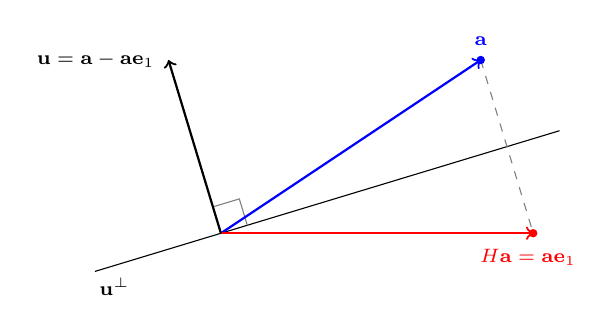
\begin{tikzpicture}
  % mirror hyperplane
  \draw[thin] (-1.60,-0.485) -- (4.30,1.302);
  \node[below] at (-1.35,-0.44) {\scriptsize $\mathbf{u}^\perp$};
  % right angle at origin
  \draw[thin,color=gray] (0.335,0.101) -- (0.234,0.436) -- (-0.101,0.335);
  % vectors
  \draw[->,thick,color=blue] (0,0) -- (3.30,2.20);
  \draw[->,thick,color=red] (0,0) -- (3.966,0);
  \draw[->,thick,color=black] (0,0) -- (-0.666,2.20);
  \draw[dashed,thin,color=gray] (3.30,2.20) -- (3.966,0);
  \filldraw[color=blue] (3.30,2.20) circle (1.3pt);
  \filldraw[color=red] (3.966,0) circle (1.3pt);
  \node[above,color=blue] at (3.30,2.26) {\scriptsize $\mathbf{a}$};
  \node[below,color=red] at (3.90,-0.08) {\scriptsize $H\mathbf{a} = \norm{\mathbf{a}}\mathbf{e}_1$};
  \node[left] at (-0.72,2.20) {\scriptsize $\mathbf{u} = \mathbf{a} - \norm{\mathbf{a}}\mathbf{e}_1$};
\end{tikzpicture}
\end{center}

\begin{method}[Householder QR]
  At the first step, let $\mathbf a_1$ be the first column of $A$ and take
  $$
  \mathbf u = \mathbf a_1 + \sign(A_{11})\norm{\mathbf a_1}\mathbf e_1,
  $$
  so that $H\mathbf a_1 = -\sign(A_{11})\norm{\mathbf a_1}\mathbf e_1$ and $HA$ has zeros below the diagonal in its first column.

  In general, suppose columns $1, \dots, k-1$ have been dealt with. Let $\tilde{\mathbf a}_k \in \R^{m-k+1}$ consist of the entries $A_{kk}, \dots, A_{mk}$ of the current $k$-th column, put
  $$
  \tilde{\mathbf u} = \tilde{\mathbf a}_k + \sign(A_{kk})\norm{\tilde{\mathbf a}_k}\mathbf e_1 \in \R^{m-k+1},
  $$
  and apply the block-diagonal orthogonal matrix
  $$
  \begin{pmatrix} I_{k-1} & 0\\ 0 & \tilde H\end{pmatrix}, \qquad \tilde H = I - \frac{2\tilde{\mathbf u}\tilde{\mathbf u}^\top}{\tilde{\mathbf u}^\top\tilde{\mathbf u}}.
  $$
  The leading $I_{k-1}$ leaves the first $k-1$ rows -- and hence the zeros already created -- untouched.
\end{method}

The choice of sign deserves comment. Either sign gives a valid reflection, but if $A_{kk}$ and $\norm{\tilde{\mathbf a}_k}$ nearly cancel then $\tilde{\mathbf u}$ is tiny and computed inaccurately. Choosing the sign of $A_{kk}$ makes the two terms reinforce rather than cancel, which is the numerically safe option.

In practice one never forms $\tilde H$ explicitly. Applying it to a vector $\mathbf v$ is just
$$
\tilde H\mathbf v = \mathbf v - \frac{2(\tilde{\mathbf u}^\top\mathbf v)}{\tilde{\mathbf u}^\top\tilde{\mathbf u}}\tilde{\mathbf u},
$$
an inner product and an axpy, costing $\mathcal{O}(m)$ rather than $\mathcal{O}(m^2)$. Similarly $Q$ itself is normally stored as the list of vectors $\tilde{\mathbf u}$, and one computes $Q^\top\mathbf b$ by applying the reflections in turn. The total cost is $\mathcal{O}(mn^2)$.

\begin{example}
  Suppose we have reached
  $$
  A = \begin{pmatrix} 2&4&7\\0&3&-1\\0&0&2\\0&0&1\\0&0&-2\end{pmatrix},
  $$
  with the first two columns already processed, and we wish to clear the third. Here
  $$
  \tilde{\mathbf a}_3 = \begin{pmatrix}2\\1\\-2\end{pmatrix}, \qquad \norm{\tilde{\mathbf a}_3} = 3, \qquad \tilde{\mathbf u} = \tilde{\mathbf a}_3 + 3\mathbf e_1 = \begin{pmatrix}5\\1\\-2\end{pmatrix},
  $$
  and $\tilde{\mathbf u}^\top\tilde{\mathbf u} = 30$, $\tilde{\mathbf u}^\top\tilde{\mathbf a}_3 = 10 + 1 + 4 = 15$. Hence
  $$
  \tilde H\tilde{\mathbf a}_3 = \tilde{\mathbf a}_3 - \frac{2\cdot 15}{30}\tilde{\mathbf u} = \begin{pmatrix}2\\1\\-2\end{pmatrix} - \begin{pmatrix}5\\1\\-2\end{pmatrix} = \begin{pmatrix}-3\\0\\0\end{pmatrix},
  $$
  and the result is
  $$
  R = \begin{pmatrix}2&4&7\\0&3&-1\\0&0&-3\\0&0&0\\0&0&0\end{pmatrix}.
  $$
\end{example}

\begin{remark}
  So which should one use? For a dense matrix, Householder: it clears an entire column with one reflection and is beautifully stable. For a matrix that is already nearly triangular, Givens: each rotation is cheap and touches only the rows that need touching. Gram--Schmidt survives mainly because it produces the columns of $Q$ one at a time, which is occasionally what one wants -- and because it generalises to infinite dimensions, where reflections do not obviously help.
\end{remark}

\subsection{Linear Least Squares}

We finish with the problem that motivated all of this. Let $A$ be $m\times n$ with $m > n$ and let $\mathbf b\in\R^m$. The system $A\mathbf x = \mathbf b$ has more equations than unknowns and generically has no solution at all; this is the situation of fitting $n$ parameters to $m$ measurements. The sensible thing to ask for instead is the $\mathbf x$ minimising the residual.

\begin{definition}[Least Squares Problem]
  Given $A \in \R^{m\times n}$ and $\mathbf b\in\R^m$, the \vocab{linear least squares problem} is to find $\mathbf x\in\R^n$ minimising $\norm{A\mathbf x - \mathbf b}_2$.
\end{definition}

\begin{theorem}[Normal Equations]\label{thm:normaleq}
  A vector $\mathbf x\in\R^n$ solves the least squares problem if and only if
  $$
  A^\top(A\mathbf x - \mathbf b) = \mathbf 0, \qquad \text{equivalently} \qquad A^\top A\mathbf x = A^\top \mathbf b .
  $$
\end{theorem}
\begin{proof}
  ($\Leftarrow$) Suppose $A^\top(A\mathbf x - \mathbf b) = \mathbf 0$ and let $\mathbf v\in\R^n$ be arbitrary. Writing $\mathbf v = \mathbf x + (\mathbf v - \mathbf x)$ and expanding,
  \begin{align*}
    \norm{A\mathbf v - \mathbf b}^2 &= \norm{(A\mathbf x - \mathbf b) + A(\mathbf v - \mathbf x)}^2\\
    &= \norm{A\mathbf x - \mathbf b}^2 + 2(\mathbf v - \mathbf x)^\top A^\top(A\mathbf x - \mathbf b) + \norm{A(\mathbf v-\mathbf x)}^2\\
    &= \norm{A\mathbf x - \mathbf b}^2 + \norm{A(\mathbf v - \mathbf x)}^2 \; \geq \; \norm{A\mathbf x - \mathbf b}^2 .
  \end{align*}

  ($\Rightarrow$) Conversely, if $\mathbf x$ is a minimiser then for every $\mathbf v$ the scalar function $t \mapsto \norm{A(\mathbf x + t\mathbf v) - \mathbf b}^2$ has a minimum at $t = 0$. Differentiating,
  $$
  0 = \left.\frac{\dd}{\dd t}\right|_{t=0}\left(\norm{A\mathbf x - \mathbf b}^2 + 2t\,\mathbf v^\top A^\top(A\mathbf x - \mathbf b) + t^2\norm{A\mathbf v}^2\right) = 2\mathbf v^\top A^\top(A\mathbf x - \mathbf b),
  $$
  and as $\mathbf v$ was arbitrary, $A^\top(A\mathbf x-\mathbf b) = \mathbf 0$.
\end{proof}

The geometric content is that the residual must be orthogonal to the column space of $A$: the best approximation $A\mathbf x$ is the orthogonal projection of $\mathbf b$ onto $\operatorname{range}A$. This is Pythagoras again, exactly as in Section 2.

\begin{center}
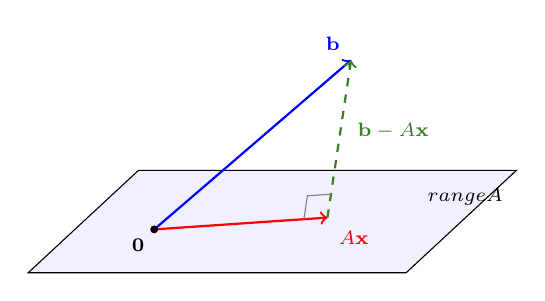
\begin{tikzpicture}
  \draw[thin,fill=blue!6] (-1.2,-0.55) -- (3.6,-0.55) -- (5.0,0.75) -- (0.2,0.75) -- cycle;
  \node at (4.35,0.42) {\scriptsize $\operatorname{range}A$};
  \draw[->,thick,color=blue] (0.4,0) -- (2.9,2.15);
  \draw[->,thick,color=red] (0.4,0) -- (2.6,0.15);
  \draw[->,thick,dashed,color=OliveGreen] (2.6,0.15) -- (2.9,2.15);
  \draw[thin,color=gray] (2.301,0.130) -- (2.345,0.427) -- (2.644,0.447);
  \filldraw[black] (0.4,0) circle (1.2pt);
  \node[below left] at (0.4,0) {\scriptsize $\mathbf{0}$};
  \node[above left,color=blue] at (2.88,2.15) {\scriptsize $\mathbf{b}$};
  \node[below right,color=red] at (2.62,0.10) {\scriptsize $A\mathbf{x}$};
  \node[right,color=OliveGreen] at (2.86,1.25) {\scriptsize $\mathbf{b} - A\mathbf{x}$};
\end{tikzpicture}
\end{center}

So one could simply solve the $n\times n$ system $A^\top A\mathbf x = A^\top\mathbf b$, say by Cholesky, since $A^\top A$ is symmetric and (if $A$ has full column rank) positive definite. This is what statisticians did for a century, and it is not wrong. But it has three defects that a numerical analyst notices immediately.
\begin{enumerate}[label=(\roman*)]
  \item Forming $A^\top A$ costs $\mathcal{O}(mn^2)$ operations and, more importantly, destroys any sparsity that $A$ possessed -- a sparse $A$ can easily have a dense $A^\top A$.
  \item The entries of $A^\top A$ are sums of products, so if the entries of $A$ vary greatly in magnitude, forming them loses accuracy through cancellation.
  \item Most seriously, the conditioning of $A^\top A$ is the \emph{square} of that of $A$. Squaring an already-large condition number is an excellent way to lose every digit one has.
\end{enumerate}

The remedy is to use the QR factorisation, which lets us minimise the residual without ever forming $A^\top A$.

\begin{theorem}[Least Squares via QR]\label{thm:lsqr}
  Let $A$ be $m\times n$ with $m \geq n$ and linearly independent columns, and let $A = QR$ be a reduced QR factorisation, with $Q$ of size $m\times n$ having orthonormal columns and $R$ upper triangular and nonsingular. Then the least squares problem is solved by the unique solution of
  $$
  R\mathbf x = Q^\top\mathbf b .
  $$
\end{theorem}
\begin{proof}
  By Theorem \ref{thm:normaleq}, $\mathbf x$ is a solution if and only if $A^\top(A\mathbf x - \mathbf b) = \mathbf 0$. Substituting $A = QR$ and using $Q^\top Q = I$,
  $$
  A^\top(A\mathbf x - \mathbf b) = R^\top Q^\top(QR\mathbf x - \mathbf b) = R^\top\left(R\mathbf x - Q^\top\mathbf b\right).
  $$
  As $R$ is nonsingular, so is $R^\top$, and the above vanishes precisely when $R\mathbf x = Q^\top\mathbf b$. That triangular system has a unique solution, found by back substitution.
\end{proof}

\begin{remark}
  Using the full QR factorisation gives the same conclusion in a way that also exhibits the residual. If $A = QR$ with $Q$ orthogonal $m\times m$ and $R = \begin{psmallmatrix}R_1\\0\end{psmallmatrix}$ with $R_1$ upper triangular $n\times n$, then since $Q^\top$ preserves norms,
  $$
  \norm{A\mathbf x - \mathbf b}^2 = \norm{Q^\top A\mathbf x - Q^\top\mathbf b}^2 = \norm{R_1\mathbf x - \mathbf c_1}^2 + \norm{\mathbf c_2}^2,
  $$
  where $Q^\top\mathbf b = \begin{psmallmatrix}\mathbf c_1\\ \mathbf c_2\end{psmallmatrix}$ is split after $n$ entries. The second term does not involve $\mathbf x$ at all, so the minimum is attained by solving $R_1\mathbf x = \mathbf c_1$, and the minimum value of the residual is exactly $\norm{\mathbf c_2}$. This is perhaps the cleanest way to see the whole result: an orthogonal change of coordinates turns an unsolvable system into a solvable one plus an irreducible remainder.
\end{remark}

\begin{example}[Fitting a Straight Line]
  Suppose we wish to fit $y = c_0 + c_1t$ to the four data points $(0,1)$, $(1,3)$, $(2,4)$, $(3,4)$. Then
  $$
  A = \begin{pmatrix}1&0\\1&1\\1&2\\1&3\end{pmatrix}, \qquad \mathbf b = \begin{pmatrix}1\\3\\4\\4\end{pmatrix},
  $$
  and the normal equations read
  $$
  \begin{pmatrix}4&6\\6&14\end{pmatrix}\begin{pmatrix}c_0\\c_1\end{pmatrix} = \begin{pmatrix}12\\23\end{pmatrix},
  $$
  with solution $c_1 = 1$, $c_0 = \tfrac32$. So the best-fitting line is $y = \tfrac32 + t$, and the residual vector is $\left(-\tfrac12, \tfrac12, \tfrac12, -\tfrac12\right)^\top$, whose components sum to zero and which is orthogonal to $(0,1,2,3)^\top$ -- exactly the two normal equations, read backwards.
\end{example}

\begin{remark}
  It is worth stepping back at the end. The least squares problem we have just solved is the same problem we solved in Section 2 with orthogonal polynomials, in a different costume: there the vector space was $C[a,b]$ or $\Pn{n}$ and the orthogonal basis was $p_0, \dots, p_n$; here it is $\R^m$ and the orthogonal basis consists of the columns of $Q$. In both cases the answer is an orthogonal projection, in both cases the good algorithm is the one that builds an orthogonal basis first, and in both cases the reason is the same -- orthogonality decouples the problem and refuses to amplify error. If there is one idea to take away from this course, it is probably that one.
\end{remark}

